\documentclass[10pt,b5paper,twoside]{book}

\usepackage[dutch,british]{babel}
\usepackage[nottoc]{tocbibind}
\usepackage{amsmath}
\usepackage{amsfonts}
\usepackage{amssymb}
\usepackage{graphicx}
\usepackage{gensymb}
\usepackage{textcomp}
\usepackage{hyperref}
\usepackage{doi}
\usepackage{xcolor}
\usepackage{xspace}
\usepackage{titlesec}
\usepackage{fancyhdr}
%\usepackage[Gray,squaren,thinqspace,thinspace]{SIunits}

\hypersetup{colorlinks=true, linkcolor=blue}
\setcounter{tocdepth}{1}

% Do not add extra vertical space
\raggedbottom

% Indent paragraphs
\setlength{\parindent}{1.0cm}

\bibliographystyle{plain_custom}

\renewcommand{\baselinestretch}{1.2}
\setlength{\parskip}{0ex plus 0.3ex minus 0.3ex}
\newcommand{\npar}{\par}
\newcommand{\mbet}{\par \vspace{1.5ex plus 0.02ex minus 0.02ex}}

% Emphasize and insert into index
\newcommand{\concept}[1]{\index{#1}\textbf{#1}\xspace}


\hypersetup{
    pdfauthor = {Ivar Clemens},
    %pdftitle = {Choosing our words},
    %pdfsubject = {Language production},
    %pdfkeywords = {language production; }
}


%% For the Chapter title, etc.
\newcommand{\bigrule}{\titlerule[0.5mm]}
\titleformat{\chapter}[display]
{\normalfont\filleft\bfseries\itshape}
{%
 \vskip-3em
\titlerule[1pt]%
\vspace{1pt}%
\titlerule
\vspace{1pc}%
\Large\MakeUppercase{\chaptertitlename} \thechapter}
{1pc}
{\titlerule
\vspace{1pc}%
\Huge}


%%%%%%%%%%%
% Document
%%%%%%%%%%%


\begin{document}

%%%%%%%%%%%%%%%
% Front matter

\frontmatter
\begin{titlepage}

\fontsize{12pt}{14pt}\selectfont

\qquad

\fontsize{17.28pt}{21pt}\selectfont

\noindent \concept{\thesistitle}
\fontsize{15.28pt}{20pt}\selectfont
 \npar \noindent \thesissubtitle

\fontsize{12pt}{14pt}\selectfont

\vspace{1cm}

\noindent \concept{Ivar Clemens}

\vspace{3cm}

\end{titlepage}

\thispagestyle{empty}

%%%%%%%%%%%%%%%%%
% COPYRIGHT PAGE

\clearpage
\pagestyle{empty}
	
\null
\vfill
\noindent ISBN: rep-la-cethi-s!-!
\npar
%\noindent Illustration: Camila Tamie Piai
%\npar
\noindent Printed by REPLACE-ME, Nijmegen, The Netherlands
\npar
\noindent \copyright 2015 Ivar Clemens %, Luc Selen, Paul MacNeilage, Mathieu Koppen, Maaike de Vrijer, Jan van Gisbergen, and Pieter Medendorp


%%%%%%%%%%%%%%%%%%%%%%%
% MANDATORY TITLE PAGE

\begin{titlepage}

\fontsize{12pt}{14pt}\selectfont
\vspace*{\fill}
\begin{center}

\fontsize{17.28pt}{21pt}\selectfont

{\textsc{\MakeUppercase{\thesistitle}}}
 \npar \MakeUppercase{\thesissubtitle}

\fontseries{m}
\fontsize{12pt}{14pt}\selectfont

\vspace{1cm}
Proefschrift
\vspace{1cm}
\npar
ter verkrijging van de graad van doctor
\npar
aan de Radboud Universiteit Nijmegen
\npar
op gezag van de rector magnificus prof. dr. Th.L.M. Engelen
\npar
volgens besluit van het college van decanen
\npar
in het openbaar te verdedigen op [dow] [dow] [month] [year]
\npar
om [hour].[min] precies
\npar
\vspace{1cm}
door
\npar
\vspace{1cm}
\concept{Ivar A.H. Clemens}
\npar
geboren op 2 juni 1984
\npar
te Boxtel, Nederland

\vspace{2.8cm}

\fontsize{17.28pt}{21pt}\selectfont

\end{center}
\end{titlepage}

\thispagestyle{empty}


%%%%%%%%%%%%%%%%%%%%%
% BACK OF TITLE PAGE

\clearpage
\pagestyle{empty}
	
\noindent \concept{Promotoren:}
\noindent \npar Prof. dr. W.P. Medendorp
\npar
\noindent \concept{Co-promotoren:}
\noindent \npar Dr. ing. L.P.J. Selen
\npar
\vspace{0.5cm}
\noindent \concept{Manuscriptcommissie:}
\noindent \npar Prof. dr. A.V. van den Berg
\noindent \npar Prof. dr. J. van der Steen
\noindent \npar Dr. S. Nooij


% Table of contents
\newpage
\renewcommand{\baselinestretch}{1.08}
\small\normalsize
\tableofcontents
\renewcommand{\baselinestretch}{1.2}
\small\normalsize


%%%%%%%%%%%%%%
% Actual text

\mainmatter
\selectlanguage{british}
\chapter{General introduction}
\newpage


The vestibular system is composed of two parts: the otoliths and the semicircular canals.

The otoliths are sensitive to linear accelearion with can in turn be cause by gravity and interial forces.

These are therefore important for the perception of: verticality, heading and displacement.

The canals are sensitive for rotational velocity and are important for 


Discuss TVOR / RVOR and relation with otoliths / canals. Neural mechanism?


Paper 1 - Linking SVV (space) and SBT (body-in-space)
Paper 3 - Influence of eye movements on self-motion perception
Paper 4 - Influence of fixation depth on self-motion perception
Paper 2 - Updating of visual stimuli across lateral translation



Overlapping themes:
  Vestibular, only otoliths; gravity (paper 1), linear acceleration (paper 2 to 4)
  Visual, orientation judgment (paper 1), updating (paper 2), self-motion (paper 3, 4)

\documentclass[10pt,b5paper,twoside]{book}


%
% Common packages and custom commands used by the main .tex files.
%

\usepackage[dutch,british]{babel}
\usepackage[nottoc]{tocbibind}
\usepackage{multicol}
\usepackage{amsmath}
\usepackage{amsfonts}
\usepackage{amssymb}
\usepackage{graphicx}
\usepackage{gensymb}
\usepackage{textcomp}
\usepackage{hyperref}
\usepackage{doi}
\usepackage{xcolor}
\usepackage{nameref}
\usepackage{xspace}
\usepackage{titlesec}
\usepackage{floatrow}
\usepackage{longtable}
\usepackage{siunitx}
\usepackage[outercaption]{sidecap}
%\usepackage{fancyhdr}
\usepackage{wrapfig}
\usepackage{lmodern}
\usepackage{multicol}
\usepackage[font={scriptsize, sf}, labelfont={sf,scriptsize,bf}]{caption}
\usepackage{src/apacite_custom}
\usepackage{src/thesis}



\pagestyle{plain}

\floatsetup[table]{font={scriptsize, sf}}

\hypersetup{colorlinks=true, linkcolor=blue, citecolor=blue}
\setcounter{tocdepth}{2}

% Do not add extra vertical space
\raggedbottom

% Indent paragraphs
\setlength{\parindent}{1.0cm}

\bibliographystyle{apacite_custom}

\renewcommand{\baselinestretch}{1.2}
\setlength{\parskip}{0ex plus 0.3ex minus 0.3ex}

\newcommand{\about}{$\approx$}

%% For the Chapter title, etc.
\newcommand{\bigrule}{\titlerule[0.5mm]}
\titleformat{\chapter}[display]
{\normalfont\filleft\bfseries\itshape}
{%
 \vskip-3em
\titlerule[1pt]%
\vspace{1pt}%
\titlerule
\vspace{1pc}%
\Large\MakeUppercase{\chaptertitlename} \thechapter}
{1pc}
{\titlerule
\vspace{1pc}%
\thispagestyle{empty}
\Huge}


\makeatletter
\renewenvironment{thebibliography}[1]
     {\footnotesize\begin{multicols}{2}[\chapter{\refname}]%
      \@mkboth{\MakeUppercase\refname}{\MakeUppercase\refname}%
      \list{\@biblabel{\@arabic\c@enumiv}}%
           {\settowidth\labelwidth{\@biblabel{#1}}%
            \leftmargin\labelwidth
            \advance\leftmargin\labelsep
            \@openbib@code
            \usecounter{enumiv}%
            \let\p@enumiv\@empty
            \renewcommand\theenumiv{\@arabic\c@enumiv}}%
      \sloppy
      \clubpenalty4000
      \@clubpenalty \clubpenalty
      \widowpenalty4000%
      \sfcode`\.\@m}
     {\def\@noitemerr
       {\@latex@warning{Empty `thebibliography' environment}}%
      \endlist\end{multicols}}
\makeatother


\hypersetup{
    pdfauthor = {Ivar Clemens, Maaike de Vrijer, Luc Selen, Jan van Gisbergen, and Pieter Medendorp},
    pdftitle = {Multisensory processing in spatial orientation:\\An inverse probabilistic approach},
    %pdfsubject = {Language production},
    %pdfkeywords = {language production; }
}

\begin{document}

\selectlanguage{british}

\thispagestyle{empty}

\chapter{Multisensory processing in spatial orientation:\\An inverse probabilistic approach}
\chaptermark{}

\newpage

\small {\bf Abstract} Most evidence that the brain uses Bayesian inference to integrate noisy sensory signals optimally has been obtained by showing that the noise levels in each modality separately can predict performance in combined conditions. Such a forward approach is difficult to implement when the various signals cannot be measured in isolation, as in spatial orientation, which involves the processing of visual, somatosensory, and vestibular cues. Instead, we applied an inverse probabilistic approach, based on optimal observer theory. Our goal was to investigate whether the perceptual differences found when probing two different states ---body-in-space and head-in-space orientation--- can be reconciled by a shared scheme using all available sensory signals. Using a psychometric approach, seven human subjects were tested on two orientation estimates at tilts \textless 120\textdegree: perception of body tilt [subjective body tilt (SBT)] and perception of visual vertical [subjective visual vertical (SVV)]. In all subjects, the SBT was more accurate than the SVV, which showed substantial systematic errors for tilt angles beyond 60\textdegree. Variability increased with tilt angle in both tasks, but was consistently lower in the SVV. The sensory integration model fitted both datasets very nicely. A further experiment, in which supine subjects judged their head orientation relative to the body, independently confirmed the predicted head-on-body noise by the model. Model predictions based on the derived noise properties from the various modalities were also consistent with previously published deficits in vestibular and somatosensory patients. We conclude that Bayesian computations can account for the typical differences in spatial orientation judgments associated with different task requirements.

\vfill

\noindent\underline{ \hspace{4cm} }

\noindent This chapter has been published as \newline
\noindent {\bf Clemens, I.A.H.}, De Vrijer, M., Selen, L.P.J., Van Gisbergen, J.A.M. and Medendorp, W.P. \citeyear{clemens2011}. Multisensory processing in spatial orientation: An inverse probabilistic approach. \emph{Journal of Neuroscience}, 31(14): 5365-5377. \newline
%\noindent Authors Clemens and De Vrijer contributed equally to this work.

\newpage

\chapter{General introduction}
\newpage

Life began about four billion years ago with the encapsulation of self-replicating RNA in a lipidic membrane \cite<e.g.>{orgel1968}. Simple as these probionts were, they did not have any means of locomotion and thus relied in full on the currents to deliver the nutrients required to replicate. As organisms evolved, they began to assert an increasing amount of control over their environment. A primitive example can be found in chemotaxis, where ciliae and flagellae, coupled with simple biochemical sensors allow the organism to follow biochemical gradients and thus actively gather nutrients.

Because flagellar motion is limited to either tumbles – random reorientation movements – or runs, the pathway linking these flagella to the biochemical sensors consists of only a few steps. With the advent of more advanced sensory and motoric systems, both the amount of information available to drive behaviour as well as the amount of possible behaviours available increased tremendously. As direct biochemical links between perception and action were no longer sufficient, simple neural network evolved to process the sensory signals allowing for abstract decisions about movement. Because organisms became more complex, these networks evolved into a complete (central) nervous system, culminating in the cerebral cortex.

In most higher organisms, including humans, the amount of data collected by the sensory organs is enormous, the visual system alone generating between $10^7$ and $10^9$ bits per second \cite{koch2006,kelly1962}. The nervous system, and the cerebral cortex in particular, seem to use probabilistic models to compress the vast amount of the incoming sensory data \cite{zhaoping2006}. The principal idea behind these models being that they reduce redundancy in the input by knowledge about the statistics of the natural world.

Predictive models, or maps, on the spatial organization of the environment are of particular interest to an organism, since they provide for example probable locations of food and predators. To use these maps, the brain needs to know both the location and orientation of the body within the environment. In this thesis, we will investigate how the brain processes the available sensory signals in the perception of gravity as well as in the internal estimation of self-motion. The goal is to build computational models and perform thorough psychometric testing in order to examine the constraints that physics and biology impose on the interaction between the vestibular and other sensory systems. 

In the following section, sensory sources for gravity and self-motion perception are described in more detail. We then elaborate on how these signals may be used and integrated in the brain, and conclude the chapter with methods for studying the processing of these signals. 
 


\section{Sensory signals for navigation}

The signals used for self-motion and orientation perception, can be split in two broad categories: absolute signals and relative signals. Absolute signals, such as landmarks, can be used to directly estimate the location and orientation of an animal while relative signals, such as acceleration, first need to be (mathematically) integrated (i.e. dead reckoning or path integration) and then used to update previous estimates of position and orientation. In the following sections the sensory system involved in position and orientation estimation will be introduced.

\subsection{Vestibular system}

While many sensory organs supply information that can be used to estimate position and orientation, there is one sensory system that evolved specifically for this purpose: the vestibular system (see \figref{intro:fig6}). It contains two sensory components, the semicircular canals and the otoliths. These sensory organs are sensitive to angular velocity and linear acceleration, respectively. Both are located in the labyrinth of the temporal bone in the inner ear.

\begin{figure}
    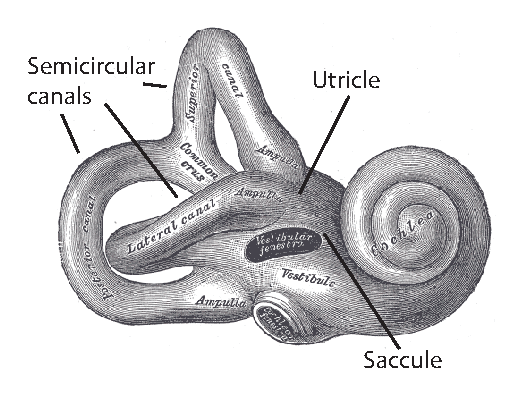
\includegraphics[width=0.5\textwidth]{src/intro/figures/vestibular.pdf}
    \caption{Schematic view of the inner ear complex consisting of the auditory system (cochlea) and the vestibular system. The vestibular system has three angular velocity (semicircular canals) and two linear acceleration (saccule and utricle) sensors.}
    \label{intro:vestibular}
\end{figure}


\subsubsection{Semicircular canals}

The semicircular canals measure the three-dimensional rotational velocity of the head. Each side of the head contains three orthogonally oriented canals allowing for rotation to be perceived in all three dimensions. Each of the six canals consists of a circular tube filled with a fluid known as endolymph (see \figref{intro:fig:canals}A). One part of the tube, the ampulla, is a bit thicker than the rest and contains a membrane, the cupula, that separates the fluid. When the head rotates, the fluid stays behind because of its inertia which in turn causes the membrane to deflect (see \figref{intro:fig:canals}B). While the inertial fluid motion suggests that the cupula should be sensitive to angular acceleration, reactive forces resulting from the fluid motion, such as endolymph viscosity and cupular elasticity,  cause the cupular deflection to reflect angular velocity instead \cite{goldberg2012}.

\begin{figure}
    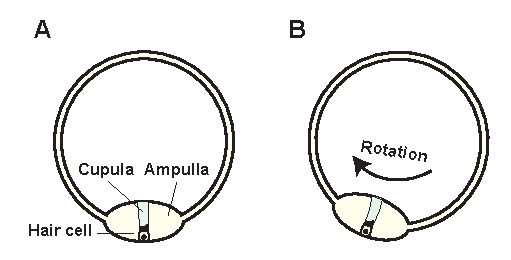
\includegraphics[width=1.0\textwidth]{src/intro/figures/canals.pdf}
    \caption{Detailed view of a semicircular canal \panelref{A} in rest and \panelref{B} during rotation. Inertia of the endolymph in the canal causes the cupula to deflect during rotation.}
    \label{intro:fig:canals}
\end{figure}

The deflection of the cupula is transduced by special hair cells which are partially embedded in the cupula. These hair cells contain bundles of small protrusions, or hairs, on their apical surface. Each bundle contains several smaller stereocilia mechanically linked to one larger kinocilium \cite{pickles1984}. When the stereocilia are stretched towards the kinocilium the links cause cation channels (mechanoelectric transducers or METs) to open and the membrane to depolarize. Glutamate is then released into the synapse and causes the afferent neuron to depolarize and, after sufficient depolarizations, to generate action potentials \cite{purves2012}. These action potentials transmit the angular velocity sensed by the canals to the central nervous system through the  vestibulocochlear nerve.

Initially, the afferent signal closely follows rotational velocity, as opposed to acceleration. During sustained rotation, the elasticity of the cupula returns it to its resting position with causes the rotational signal to subside slowly. This is partly compensated for through velocity storage in the central nervous system \cite{goldberg2012}. The canals are only sensitive to changes in orientation, as their circular nature makes them insensitive to the effects of linear acceleration and gravity \cite{goldberg2012}. 


\subsubsection{Otoliths}
The linear acceleration and gravitational forces are measured by the two otolith organs on either side of the head: the saccule and the utricule. Each otolith consists of an endolymph filled compartment containing calcium carbonate crystals known as otoconia (\figref{intro:fig:otoliths}A). Due to their high inertia, these otoconia fall behind during linear acceleration (\figref{intro:fig:otoliths}B), and move ahead during deceleration. In addition, they fall downward as a result of the gravitational field (\figref{intro:fig:otoliths}C). The otoconia are mounted on top of a flexible polysaccharide gel, in which hair cells, similar to those found in the semicircular canals, are partly embedded \cite{goldberg2012}.  

Einstein's equivalence principle states that  it is not possible to measure forces caused by linear acceleration and by gravity independently. The signal coming from the otoliths is therefore proportional to the combination of these forces \cite{fernandez1976b}, which is commonly referred to as the gravito-inertial force (GIF). Compared to the three semicircular canals, which are able to sense rotation in three dimensions due to their orthogonal organization, either side of the head only contains two otolith organs. It is still possible to sense the gravitoinertial force in three dimensions because the otolith organs are curved, and the orientation of the hair cells determined the direction of sensitivity \cite{goldberg2012}.

\begin{figure}
    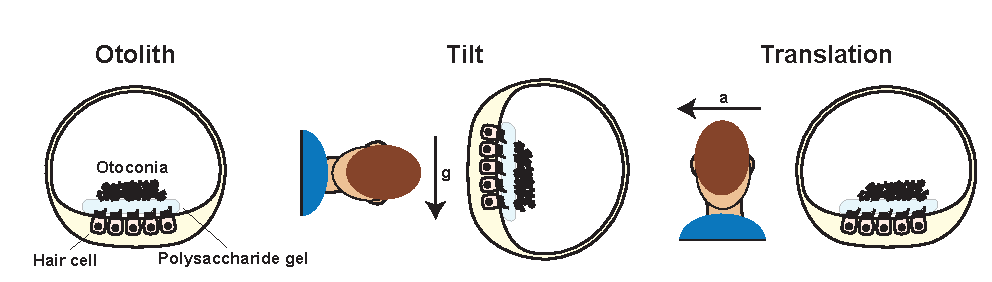
\includegraphics[width=1.0\textwidth]{src/intro/figures/otoliths.pdf}
    \caption{Detailed view of an otolith \panelref{A} in rest, \panelref{B} during head tilt, and \panelref{C} during linear acceleration. The high inertia of the otoconia keeps them from moving rapidly during both head tilt as well as linear acceleration. As the effect is physically identical in either case, head tilt and linear acceleration cannot be disambiguated based on the otolith signal alone.}
    \label{intro:fig:otoliths}
\end{figure}

For many actions, the brain needs to disentangle the contributions of gravity and linear acceleration to the gravitointertial force. For example, the linear vestibuloocular reflex (LVOR) that stabilizes gaze during translation should be sensitive to translation while ignoring gravity. Under normal circumstances, the brain is able to perform this task well \cite{merfeld1995}, but during extreme conditions such as in airplanes or space flight errors might occur. The somatogravic illusion \cite{glasauer1995} is an example of a disambiguation error. In this illusion an airplane accelerates forward which causes an inertial force in the opposite direction. The direction of the resulting GIF will therefore be in between gravity (downward) and the intertial force (backward). The brain erroneously interprets the (majority of the) GIF as being caused by gravity, leading to the perception of "nose-up" pitch tilt.

Various theories have been proposed as to how the brain might solve the tilt-translation ambiguity. The frequency segregation hypothesis, for example, makes use of the fact that when stationary, the only force we experience is gravity. In this case, sustained (low frequency) accelerations should be  attributed to gravity, while the high frequency components should be attributed to translation \cite{paige1991, telford1997}. Other models keep track of the expected direction of gravity by integrating over the vector product of gravity and angular velocity from the semi-circular canals, and subtracting that signal from the otolith signal to obtain an estimate of linear acceleration. Because the semi-circular canals play a  crucial role in these models, they are known as multisensory integration models \cite{mayne1974,ormsby1977}. Merfeld and Zupan \citeyear{merfeld1995,merfeld2002} further refined the multisensory integration model by explicitly stating that the brain uses an (internal) model of the physical world to resolve the tilt-translation ambiguity.

The disambiguation of linear acceleration and gravity is not solely based on vestibular inputs, but also takes the  range of  possible movements into account. For example when moved on a linear sled, the probability of a participant perceiving tilt is greatly reduced \cite{wertheim2001}, indicating that cognitive processes also influence disambiguation.


\subsection{Somatosensory}
The gravito-inertial force (GIF) caused by a combination of gravity and linear acceleration is not only detected by the vestibular system, but also sensed by other sensory systems. Early evidence that non-vestibular sources were used by the brain came from DeKleyn and Versteegh \citeyear{dekleyn1933} who showed that inertial reflexes still occurred after removal of the otolith organs.

Since then, the contribution of specific organs to GIF perception has been demonstrated. In 1992, \citeauthor{mittelstaedt1992} rotated supine participants along  their naso-occipital axis,  causing  the centrifugal force to act on somatic GIF sensors  but not on the otoliths. In nephrectomized participants, the perceived direction of gravity relied less on the centrifugal force compared to controls, suggesting that the kidneys play a crucial role in perception of the gravitointertial force. Further evidence came from Trousselard \citeyear{trousselard2004}, who showed that the perception of gravity in a tilted position depends on whether the stomach is full or empty. In addition, reducing somatosensory cues, by applying a body cast, also affects the perception of gravity \cite{trousselard2004}.  Similar results have been obtained for many other visceral factors, such as the blood vessels \cite{vaitl2002}, and spinal axis fluid \cite{vaitl1997}.


\subsection{Visual}
Even though the vestibular and somatosensory systems directly measure the gravito-inertial force, orientation and navigational information can also be extracted from the visual system. In many cases, especially when the low latency of the vestibular signal is not required, the visual signal even overshadows the vestibular one \cite{wright2005,gaerlan2012}.

\subsubsection{Vection}
When we move through the environment, the image of the world on our retina shifts. This large-field shift pattern, also known as optic flow, depends on the movement being made. Lateral translation (\figref{intro:fig:vection}A) for example causes a different pattern than roll rotation (\figref{intro:fig:vection}B). At the turn of the 19th century von Helmholtz \citeyear{vonhelmholtz1867} recognized the importance of these flow signals for self-motion perception. In some cases the optic flow signal is so strong that it causes a percept of self-motion in stationary participants, called vection \cite{dichgans1978}. This is experienced, for example, when sitting on the train and a neighbouring train starts to move. This effect is much less likely to occur when e.g. on the platform, suggesting that the vection signal is integrated with prior knowledge about the environment before causing self-motion perception \cite{andersen1985,lepecq1995}


\begin{figure}
    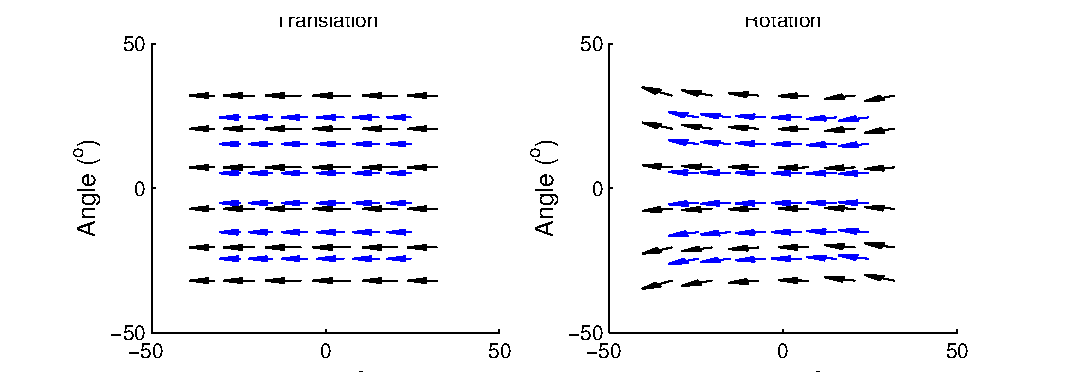
\includegraphics[width=1.0\textwidth]{src/intro/figures/optic_flow.eps}

    \caption{Vection pattern during \panelref{A} lateral translation and \panelref{B} rotation. During translation nearby targets (red) have a larger retinal displacement compared to far away ones (blue). Retinal displacement across rotation does not depend on target distance. }
    \label{intro:fig:vection}
\end{figure}

Similar retinal shifts are also observed during movement of the eyes or head. When interpreting optic flow the brain needs to distinguish object- from self-motion, this process is called optic flow parsing. One strategy is to use extra-retinal cues such as the vestibular, and somatosensory signals to subtract out the retinal stimulation due to self-motion \cite{wertheim1994,wexler2001,macneilage2012}.

While the extra-retinal information does contribute to optic flow parsing, the existence of vection \cite{dichgans1978} suggests that the brain can parse optic flow using a purely visual approach \cite{rushton2005,warren2007}. Warren and Rushton \citeyear{warren2009} have shown that the brain indeed uses the global pattern of retinal motion caused by self-motion to parse optic flow. Even though global retinal flow patterns are used to disambiguate between object- and self-motion, it does not mean that a percept of self-motion, i.e. vection, exists. Research has shown that vection can take up to 30s to establish, but that purely visual optic flow parsing occurs within 1s \cite{warren2009}.

\subsubsection{Landmarks}
In addition to relative cues, the brain seems to use absolute cues in both the perception of gravity and self-motion. For the perception of gravity, it makes use of the fact that many lines within the world are aligned with either the horizon or gravity (\figref{intro:fig:treeframe}A). Straight lines therefore acts as a priors attracting the perceived direction of gravity towards them. A special case is the rod-and-frame illusion (\figref{intro:fig:treeframe}B), where the perceived angle of a rod relative to gravity is affected by the orientation of the frame that contains it \cite{witkin1948}. 

\begin{figure}
	\includegraphics[width=1.0\textwidth]{src/intro/figures/treeframe.pdf}
	\caption{\panelref{A} Trees are aligned with gravity, making them ideal cues for orientation. \panelref{B} The rod-and-frame illusion; even though the frame is rotated, participants might perceive the line as being slanted.}
	\label{intro:fig:treeframe}
\end{figure}

Similarly, our position within the world can be established using world-fixed landmarks. With the exception of animals and vehicles, most items in the world rarely change position. By comparing our current visual scene (e.g. Sequoia trees in \figref{intro:fig:treeframe}A) with our knowledge about the environment we can determine our location (in this case northern California). Because the experiments outlined in this thesis were performed in near darkness, these absolute navigational cues can be considered less relevant. 


\subsubsection{Oculomotor}
Self-motion is typically accompanied by eye movements that help to improve dynamic visual acuity and reduce retinal slip. In Chapter 3 of this thesis, we explore whether these eye movements may have a reversed role, providing cues about self-motion perception beyond optic flow parsing. 

In 1963, \citeauthor{guedry1963} reported a substantial underestimation of displacement when their observers watched a small body-fixed target compared to displacements in the dark. Because of the VOR, eye movement in darkness are larger than those in the body-fixed condition. The underestimation in the body-fixed condition can therefore be interpreted as the involvement of eye movements, although the authors did not suggest this 
Studies on postural sway also indicate a role of eye movement is self-motion perception. Making eye movements causes postural sway to increase, suggesting that eye movements influence self-motion perception \cite{glasauer2005,rodrigues2015}.

One complication is that the magnitude, $e$, of these eye movements not only depend on the translation amplitude, $T$, but also on the fixation depth, $d$. When fixating position $(x, d)$, the eye position at starting position is $e_0 = atan(d/x) \approx d/x$. By subtracting the eye position after the translation, $e_1 = atan(d/(x+T)) \approx d/(x+T)$, we obtain the eye movement amplitude, $e \approx d/T$. In Chapter 4 we explore whether the brain takes this geometry into account and compensates for fixation depth when using eye movements in self-motion perception.


\section{Reflexive uses for the self-motion}
While vection is a valuable cue to self-motion perception, the brain wants to minimize vection because it blurs the image on the fovea, which hampers visual perception. Several reflexive mechanisms attempt to keep stable fixation to avoid image blurring during self-motion. Two such mechanisms are the vestibulo-ocular reflex, the VOR, and the optokinetic reflex, the OKR.

The vestibulo-ocular reflex (VOR) is driven by the short-latency vestibular signal and compensates for both rotation and translation of the head. The rotational and translational part of the VOR have their own dedicated reflex arcs. The translational VOR, or TVOR, is driven by the otolith signal while the rotational VOR, or RVOR, is mainly driven by the semicircular canals. The RVOR operates during head rotation by counter rotating the eyes in the opposite direction to the head. Because its gain is about one, eye velocity is about equal, but of opposite sign, to the head velocity. The TVOR operates during head translation, when the head moves orthogonally to the line of sight. In contrast to the RVOR, the TVOR needs to take fixation depth into account. Simple geometry shows that the ideal TVOR response is inversely proportional to fixation distance, $e_{vor} = atan⁡(d/T)$. As a result, no compensatory eye movements are required when fixating targets at infinity to maintain a stable retinal image. 

The optokinetic reflex is driven by optic-flow, and also compensates for both translational and rotational movement. Because the cells driving the OKR are more sensitive to slow motion, the OKR compensates predominantly for the low frequency components of movements. While the VOR dies away during sustained rotation, the OKR remains because it is sensitive to constant velocity stimuli \cite{soodak1988}.

The eye movements that are induced by the OKR and the VOR consist of two parts; a slow-phase pursuit-like movement which keep the eyes on target and quick-phase saccades which quickly move the eyes back after they lost track due to physical constraints of the oculomotor system \cite{goldberg2012}.

\section{Integration of signals for action and perception}

While reflexes by definition depend on minimally processed sensory signals, higher animal functions can rely on more elaborate processing. One such processing step is determining the underlying physical cause of a sensory signal. Multiple sensory systems provide information about the same physical quantity. For example, both the visual and the vestibular system provide information about self-motion. Two very naive approaches to derive a self-motion percept from these signal whould be to solely rely on the most reliable cue and ignore the others or to just average the available signals. A better solution, however, is to weigh all available signals by their  relative reliabilities and combine them with a-priori knowledge about the probability of specific self-motion states. This approach is known as statistically optimal, or Bayesian, integration. 

We will now briefly explain the mathematical foundations of optimal integration. Suppose there is a true physical stimulus in the world, $x$, which is observed by multiple sensory systems, $x_i$. We assume that these observations are corrupted by independent Gaussian noise, $\sigma_i^2$. The probability of the observations, $x_i$, given the stimulus $x$, is therefore:

\begin{equation}
P(x_i|x)= \mathcal{N}(x_i, \sigma_i^2)
\end{equation}

From the point of view of the brain, the observations, $x_i$, are given while the stimulus, $x$, has to be inferred. In this case, probability $P(x_i│x)$ is referred to as the likelihood of  the  stimulus given the observations, or $\mathcal{L}(x|x_i)$. Given multiple sensory observations, $x_1,...,x_n$, we can now compute the likelihood of the stimulus:

\begin{equation}
\mathcal{L}(x|x_1,...,x_n) = P(x_1,...,x_n|x) = \prod_i P(x_i|x)
\end{equation}

Making use of Bayes' rule, the  brain can infer the probability of the stimulus given its observations:

\begin{equation}
P(x|x_1,...,x_n) = \frac{P(x_1,...,x_n)P(x)}{P(x_1,...,x_n)}
\end{equation}

In this equation, $P(x)$ represents the prior probability of the stimulus, that is the probability of the stimulus occurring without taking the sensory input into account. The left-hand side of the equation, $P(x│x_1,..,x_n$, is commonly referred to as the posterior probability.

The  most likely stimulus given the observations is  the one for which the posterior probability is largest. This method of finding the most optimal estimate (\eqnref{intro:eq:map}) is known maximum a posteriori estimation (MAP).

\begin{equation}
\hat{x} = argmax_x P(x_1,...,x_n|x)P(x)
\label{intro:eq:map}
\end{equation}

When using a flat prior, that is when all stimuli are equally likely to occur, $P(x)=c$, \eqnref{intro:eq:map} can be simplified to

\begin{equation}
\hat{x} = argmax_x P(x_1,...,x_n|x)
\label{intro:eq:mle}
\end{equation}

In this case, we refer to it as maximum  likelihood estimation (MLE). The solution for the  most likely stimulus, $\hat{x}$, is a weighted sum of the sensory inputs,

\begin{equation}
\hat{x}=\sum_i w_i x_i
\end{equation}

with weight, $w_i$,

\begin{equation}
w_i = \frac{1/\sigma^2_i}{\sum_j 1/\sigma^2_j}
\end{equation}

As the posterior is a distribution, it also provides us with an estimate of uncertainty in  the most likely stimulus value,

\begin{equation}
\hat{\sigma}^2_i = \frac{\prod_i \sigma^2_i}{\sum_i \sigma^2_i}
\end{equation}

In many cases the brain does not use a flat prior, but a Gaussian one. For example, in Chapter 2, we use a prior ... head is upright in space.

%%%%%%%%%%%%%%%%%%%%%%%%%%%%%%
%
% Add a bit more about optimal integration, perhaps give an example?
%

In this case, the Gaussian prior can be seen as an additional sensory signal that is weighted into the posterior estimate.


\section{Studying the link between sensory signals and perception}

A large part of our knowledge on the relation between perception and sensory processing comes from psychophysical experiments. In this type of experiments the relation between physical stimuli, e.g. the true angle of the body relative to gravity, and perception, e.g. perceived body orientation, is quantified.

A powerful tool in psychophysical research is the two-alternative forced choice, or 2AFC, paradigm. In this paradigm, participants are presented with two stimuli, e.g. two translation distances, and are then forced to make a choice, e.g. on which of the two translations was longer. By systematically varying one of the choice alternatives (i.e., the probe stimulus), the point of subjective equality, or PSE, can be determined. The PSE is the point at which the participant is completely unsure about which stimulus to pick, i.e. gives a random response, because he perceives the two stimuli as being equal. If the PSE does not line up with the actual reference stimulus, there is a bias in the percept, represented by the Greek letter mu ($\mu$).

In addition to establishing perceptual equality, the 2AFC paradigm also allows for quanifying the uncertainty in perception by looking at the slope of the psychometric curve around the PSE. This uncertainty is commonly quantified by the standard deviation of the cumulative Gaussian probability distribution that underlies the responses of the subject, represented by the Greek letter sigma ($\sigma$).

%%%% Include some equations?

The next three sections will introduce the three 2AFC tasks that are central in the present work.

\subsection{Subjective body tilt}
In the subjective body tilt, or SBT, task the perceived body orientation with respect to a given body tilt angle is probed. Participants are first given a reference angle, e.g. 45 \si{\degree}, and are then rotated to an angle close to the reference angle, e.g. 46 \si{\degree} (see \figref{intro:fig4}A). They then have to indicate whether their current orientation is clockwise or counter-clockwise with respect to the reference angle. By systematically probing rotation angles around the reference angle we can obtain both the bias and uncertainty on the percept of body tilt.

Most participants are able to do this perfectly, regardless of the reference angle (see \figref{intro:fig4}B). Their uncertainty does increase as a function of reference angle though (see \figref{intro:fig4}C).
As the SBT probes body orientation, the somatosensory signal originating from the torso can be used without any reference transformation and thus provides a direct contribution. Other sensory signals such as the vestibular signal can also be used, but only after a reference frame transformation.

\begin{figure}
    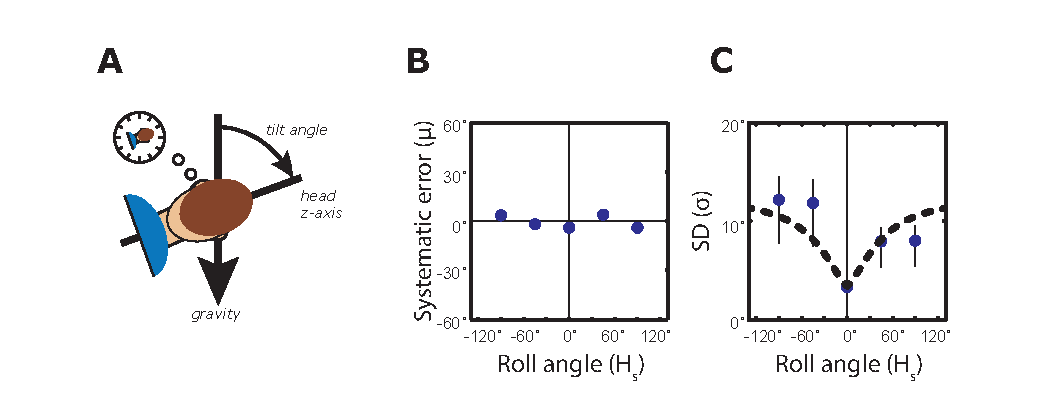
\includegraphics[width=1.0\textwidth]{src/intro/figures/sbt.pdf}

    \caption{Subjective body tilt task (SBT); \panelref{A} Graphical representation of the SBT task. \panelref{B} Bias and \panelref{C} uncertainty as a function of roll angle in a typical participant (circles). The dashed line represents the typical pattern.}
    \label{intro:fig4}
\end{figure}


\subsection{Subjective visual vertical}
The subjective visual vertical, or SVV, task is a similar task in which participants have to judge the orientation of a line with respect to gravity. The PSE, that is the angle at which the line is perceived to be aligned with gravity, can be found by presenting lines at different angles and asking the participant whether the line is rotated clockwise or counter-clockwise relative to gravity (see \figref{intro:fig5}A).

When seated straight this task, participants do not make any static errors and are very certain about their responses (see \figref{intro:fig5}B and C). This changes when first rotating the participant before the task. In general, the static error increases with tilt angle, the direction of the error is in the direction of the body mid-line, this effect is known as the Aubert or A-effect. At smaller angles overcompensation occurs and the static error moves in the opposite direction, that is away from the body mid-line. This latter effect is known as the E-effect and could be due to the effects of ocular counter-roll (OCR).

\begin{figure}
    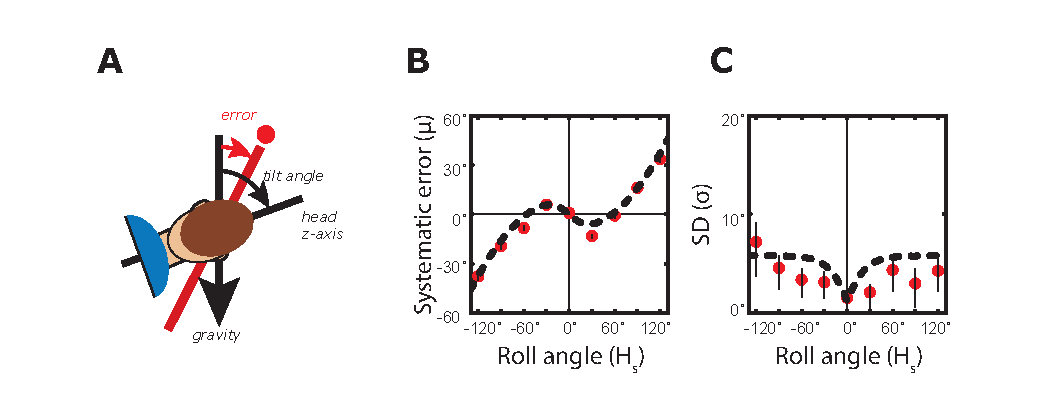
\includegraphics[width=1.0\textwidth]{src/intro/figures/svv.pdf}

    \caption{Subjective visual vertical task (SVV); \panelref{A} Graphical representation of the SVV task. \panelref{B} Bias and \panelref{C} uncertainty as a function of roll angle in a typical participant (circles). The dashed line represents the typical pattern.}
    \label{intro:fig5}
\end{figure}

\subsection{Translation perception}

Perhaps explain the lateral translation task.


\section{Outline of this thesis}

Both the estimation of body orientation and self-motion require the integration of multiple sensory signals. This thesis explores how the brain weights and integrates the different sensory signals to form dynamic but coherent percepts of self-motion and orientation.

We start with Chapter 2 in which we investigate sensory noise levels of the visual, somatosensory, and vestibular cues to head and body orientation. Because the contributions of these signals cannot be studied in isolation, we adopted an inverse approach where we assumed statistical optimality and attempted to compute the statistical properties of individual sensors. To this end, we fitted an optimal integration model to the behaviour from two psychophyisical tasks. The first gauged head-in-space orientation (SVV) and the second body-in-space orientation (SBT). The resulting estimates of the noise levels in the involved sensory modalities were used to predict the responses of patients with somatosensory and vestibular deficits. These predictions were consistent with previously published deficits for these patient groups, strengthening the idea that human spatial orientation is statistically optimal.

In Chapter 3 we example the dynamic aspects of the integration of vestibular and non-vestibular cues for self-motion perception. We specifically focus on the contributions of eye movements to the perception of whole-body translation. Using a psychophysical task, we first show that translations in which the eyes fixate a body-fixed target are perceived as shorter than those in which the eyes fixate a world-stationary target and thus make pursuit movements. We further demonstrate that this result does not depend on the presence of the fixation point per se, but that the magnitude of unconstrained eye movements in complete darkness directly influences the self-motion percept. 

Because fixation distance influences the magnitude of pursuit eye movements, we investigated  whether the brain takes fixation distance into account in Chapter 4. We compared self-motion perception during near and far world-fixed targets. Results suggest that fixation depth is only partially taken into account in the integration of vestibular and non-vestibular information for the calculation of translation distance. It seems that only raw eye movements augment self-motion perception, resulting in a biased percept.

Chapter 5 presents the final experimental study of this thesis, where we investigate how self-motion signals are used to update the location of previously seen objects across whole-body translation. We show that the errors made during spatial updating do not only depend on the location of the previously seen object, but also on the location of gaze. This is consistent with spatial updating in a gaze-centred reference frame. We further show that the underestimation of self-motion is a possible cause of the errors found.

\section{Materials and Methods} \label{sec:mm}

\subsection{Subjects}

Seven subjects (6 male, 1 female) provided written informed consent to participate in the experiments. Ages ranged from 23 to 65 years. Subjects were free of any known vestibular or other neurological disorder and had normal or corrected-to-normal visual acuity. All subjects took part in SBT and SVV experiments (see below, Experiments) and returned to the laboratory for an independent measurement of neck proprioception. Before each experiment started, subjects received careful instructions and performed a few practice runs to get used to the task. Participants never received any feedback about their performance, not even in the training trials. Each subject participated in 20 experimental sessions of {\textasciitilde}45 min each, yielding {\textgreater} 15 h recording time per participant.
%%% ^^ Needs fixing

\subsection{Setup}

Body tilt was controlled by a computer-controlled vestibular chair, which was configured to allow subject rotation in the roll axis. A digital position encoder measured roll position with an angular resolution of 0.04\textdegree. The subject's body was tightly fixated using a five-point seat belt and adjustable shoulder and hip supports. Velcro straps restrained both legs and feet, and a padded helmet firmly fixated the head in a natural upright position for looking straight ahead. Subject-specific seat adjustments ensured that the naso-occipital axis, midway between the eyes, coincided with the roll axis of the chair. Experiments took place in complete darkness. 

\subsection{Experiments}

\subsubsection{SBT} \label{sec:mm:exp:sbt}
 
The SBT experiment served to obtain a psychometric measure of each subject's accuracy and precision of body-tilt perception at five body-tilt angles: upright (0\textdegree, SBT0 task) and 45\textdegree and 90\textdegree right side and left side down (SBT\textpm45 task and SBT\textpm90 task). Negative angles indicated left side down. We applied the method of constant stimuli, using a set of 10 equidistant body-tilt angles, centered on tentative estimates of the subject's 0\textdegree (SBT0), 45\textdegree  (SBT45), -45\textdegree (SBT-45), 90\textdegree (SBT90), and -90\textdegree (SBT-90) body-tilt percept. The latter were determined in a few pilot trials that also served to familiarize the subject with the task, without providing a reference of the five respective orientations to be tested. Relative to the test angle, we used test angle intervals of 3\textdegree, 4\textdegree, and 4\textdegree  in the SBT0, SBT\textpm45, and SBT\textpm90 tasks, respectively. Body-tilt angles were tested 14 times in random order, yielding 140 responses for each psychometric curve. 

To perform the psychophysical SBT experiments, two methodological problems had to be solved. The first relates to the number of experimental sessions that we could reasonably ask subjects to perform. We realized that returning the subject to upright for reorientation after each trial would require too large a number of experimental sessions. Our overriding concern was that starting each trial from upright would confound the SBT0 task in the sense that subjects could then simply notice the change in chair position. To prevent this, we always inserted a detour rotation before moving the subject to the test angle in a given trial. The detour, always to a tilt position clearly outside the psychometric test range, served to reset the subject's memory of the previous tilt position. These detour angles were chosen randomly from a range at 30-40\textdegree clockwise (CW) and counterclockwise (CCW) from the presumed threshold. As an illustration, Figure 2 shows how the subject was moved from one trial to the next in the course of an SBT90 experiment. Detour angles preceding each test angle were taken from the CW and the CCW detour range in equal proportions. An analysis of trial history effects indicated that detour angles did not affect the judgment in the subsequent trial ($p > 0.05$). 

%\begin{figure}
\begin{wrapfigure}{l}[5pt]{0.5\textwidth}
    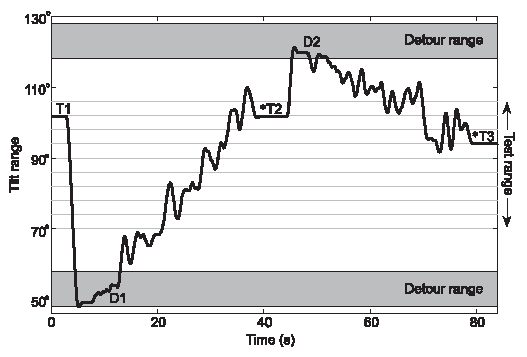
\includegraphics[width=0.5\textwidth]{src/paper1/figure2.pdf}
    
    \caption{Tilt paradigm in $SBT_{90}$ task. T1, T2, T3, Test angles at which the subject was prompted with a beep signal (*) to indicate whether body orientation was CW or CCW from the instructed reference orientation (i.e., 90\textdegree in this example). D1, D2, Detour angles randomly drawn from detour range (30 – 40\textdegree CW and CCW from center of test range). Rotations from detour (D) to test (T) angle were performed in a noisy fashion (see Materials and Methods, SBT).}
%\end{figure}
\end{wrapfigure}

Each experimental run started in upright position with the room lights on. After the lights were turned off, subjects were first rotated at a constant angular velocity of 30\textdegree/s to a random detour angle, outside of the test angle range, where they remained for 3 s. The chair then moved to a randomly chosen position within the test range with a very slow and noisy profile, defined by the sum of a ramp of 0.4-2\textdegree/s and Gaussian white noise (bandwidth, 0-0.7 Hz; RMS amplitude, 3.4\textdegree). Ramp speed was chosen such that the trajectory between detour angle and test angle was reached in 30 s (Fig. 2). These precautions were taken to enforce independent absolute tilt judgments and to deter reliance on sensed changes in tilt position that had occurred since the previous trial. Three seconds after arrival at the test angle, a beep signal prompted the subject to indicate whether body orientation was CW or CCW from the instructed reference orientation (0\textdegree in the SBT0 task, \textpm45\textdegree in the SBT\textpm45, or ±90\textdegree in the SBT\textpm90 task), using a toggle switch. The subject was then rotated at a constant velocity to a new randomly drawn detour angle, and the above procedure was repeated. Each run, comprising seven test angles, lasted ~5 min, after which the subject was rotated back to upright, and room lights were turned on. Between runs, there was a 60 s rest interval before the next run started. Each SBT task was tested in separate sessions of \textasciitilde45 min each, thus amounting to a total of 15 sessions per subject (i.e., \textasciitilde11 h of recording time). 
% ^ Needs fixing

\subsubsection{SVV} \label{sec:mm:exp:svv}
 
The same subjects were also tested in a series of SVV experiments. Part of this dataset (four subjects) has been published previously as part of a larger dataset on visual verticality perception (De Vrijer et al., 2009). Data in the other three subjects were collected anew. Here we provide a brief summary of the paradigm. SVV was tested at nine roll-tilt angles, ranging from -120 to 120\textdegree at 30\textdegree intervals. A luminous line (angular subtend, 20\textdegree), polarized with a bright dot at one end, was mounted in front of the subject. The line's rotation axis coincided with the chair rotation axis. In each experimental run, the subject was rotated from upright to the chosen test angle at a constant angular velocity of 30\textdegree/s. After a 30 s waiting period that allowed canal effects to subside, a luminous line was briefly flashed (20 ms), and the subject indicated whether its orientation in space was CW or CCW from the perceived direction of gravity. The line orientation was selected randomly from a set of 11 line orientations. After all line orientations had been tested, the subject was rotated back to upright, and room lights were turned on. Positive and negative body-tilt angles were alternated regularly. As in the SBT experiment, we used the method of constant stimuli. The set of 11 line orientations was centered on a coarse estimate of the SVV threshold at each tilt angle. We used orientation intervals of 3∞, except for upright, where intervals of 2\textdegree were taken. Each set of line orientations was tested in random order in 12 experimental runs, thus yielding a total of 132 responses for each psychometric curve. SVV data were collected in a total of five 45 min sessions per subject. 

\subsection{Data analysis} \label{sec:mm:da}

CW tilt angles of the body and the luminous line were defined positive. We quantified performance, for each roll-tilt angle (5 in the SBT and 9 in the SVV) independently, by examining the proportion of CW responses as a function of body orientation (SBT) and the proportion of CCW responses as a function of line orientation with respect to the body (SVV). Psychometric data were quantified by fitting a cumulative Gaussian function (Fig. 3): 

\begin{equation}
\label{p1eqn1}
P(x) = \lambda + (1 - 2\lambda) \frac{1}{\sigma \sqrt{2\pi}} \int_{-\infty}^{x}{e^{-(y-\mu)^2 / 2\sigma^2}}dy,
\end{equation}
% Equation 1


in which $x$ represents body orientation in space (SBT experiment) or line orientation with respect to the body (SVV experiment). The mean of the Gaussian $\mu$ represents the subjective perception of the reference orientation in the SBT task, or the SVV compensation angle (the angle between the apparent visual vertical line and the body axis) in the SVV task. The width of the curve, $\sigma^2$, inversely related to precision, serves as a measure of the subject's variability in the SBT or SVV task. Parameter $\lambda$, representing the lapse rate, accounts for stimulus-independent errors caused by subject lapses or mistakes and was restricted to small values ($\lambda < 0.06$). Fits were performed using Matlab software (MathWorks) with the routine ``psignifit'' \cite{wichmann2001b}. 

\subsection{Sensory integration model}

To provide a theoretical framework that explains the observed responses, we designed a sensory integration model for visual verticality and body-tilt perception that assumes optimal processing of all potentially relevant sensory signals, including body, head, and neck sensors. The model links accuracy and variability in the two spatial tasks to the properties of the underlying sensors. For simplicity, the scheme is limited to SBT and SVV signal processing in darkness. 

In the scheme (Fig. 1), we use the following conventions: physical variables are denoted by a capital with a subscript indicating the frame of reference. For example, $H_S$ represents the physical orientation of the head in space. Sensory signals and their reference-frame-transformed counterparts are denoted by a hat symbol ($\hat{}$), as in $\hat{H}_{S}$, which represents the orientation of the head in space as measured by the head-in-space sensors. The optimal estimate of a variable, obtained by integration of all available information, is indicated by a tilde ($\sim$), as in $\tilde{H}_S$, representing the final head-in-space estimate. 

It is assumed that all sensory signals are accurately calibrated (i.e., unbiased) but corrupted by independent Gaussian noise with a given variance ($\sigma^2$), with subscripts to indicate the sensory modality (e.g., $\sigma_{BS}^2$ represents noise variance in the body-in-space sensors). 

\subsubsection{SBT computation}
\label{sec:sbt_computation}
 
To obtain an estimate of the orientation of the body in space, the brain can use ``direct'' sensory information from body sensors ($\hat{B}_S$), such as tactile receptors in the skin or so-called graviceptors in the trunk \cite{mittelstaedt1997, mittelstaedt1998, vaitl2002}. Alternatively, an ``indirect'' pathway, involving a reference frame transformation, can also provide a body-in-space estimate. For this purpose, sensory head-in-space information, provided by the otoliths, must be combined with information about head-on-body orientation, provided by proprioceptive signals from the neck ($\hat{B}_{SI} = \hat{H}_S - \hat{H}_B$). Because the sensors are contaminated by noise, the direct and indirect signals can be represented as Gaussian probability distributions with mean values of $\hat{B}_S$ and $\hat{H}_S - \hat{H}_B$, and variance levels of $\sigma_{BS}^2$ and $\sigma_{HS}^2 + \sigma_{HB}^2$, respectively. Theoretically, as shown in Figure 1, the brain could also use prior information about body-in-space orientation in the computation of the body-in-space estimate. The effect of including a prior on the SBT (centered on upright) would be a systematic error of underestimation at larger tilt angles. However, neither previous findings \cite{mittelstaedt1983, mast1996, jarchow1999, vanbeuzekom2001} nor the present results (Figs. 3, 4), showed such systematic errors across subjects. In modeling terms, this indicates a uniform (uninformative) prior, which corresponds to a weight of 0. Accordingly, a statistically optimal estimate of body-in-space orientation ($\tilde{B}_S$) is then given by the peak of the Gaussian distribution that results from the multiplication of the two distributions representing the direct and indirect sensory pathways. It follows that

\begin{equation}
\label{p1eqn2}
\tilde{B}_S = w_{BD} \cdot \hat{B}_S + w_{BI} \cdot (\hat{H}_S - \hat{H}_B),
\end{equation}

with

\begin{equation}
\label{p1eqn3}
w_{BD} = \frac{1/\sigma^2_{BS}}{1/(\sigma^2_{HS} + \sigma^2_{HB}) + 1/\sigma^2_{BS}}
\end{equation}

and

\begin{equation}
\label{p1eqn4}
w_{BI} = \frac{1/(\sigma^2_{HS} + \sigma^2_{HB})}{1/(\sigma^2_{HS} + \sigma^2_{HB}) + 1/\sigma^2_{BS}}
\end{equation}

in which $w_{BD}$ and $w_{BI}$ (Fig. 1) represent the respective weights of the direct and indirect pathways, which add up to 1 \cite{landy1995,jacobs1999,ernst2002,bays2007}. Note that the weight of each pathway depends on its reciprocal noise variance (also known as precision), so that precise signals have a stronger influence on the final estimate than noisy signals. Furthermore, because both sensory pathways are supposed to carry unbiased signals, the mean estimate of body in space in multiple trials, $\mu(\tilde{B}_S)$, will also be accurate. 

It can further be shown that the variance in $\tilde{B}_S$ in multiple trials, denoted as $\sigma^2(\tilde{B}_S)$, equals 

\begin{equation}
\label{p1eqn5}
\sigma^2(\tilde{B}_S) = \frac{
\sigma^2_{BS} \cdot (\sigma^2_{HS} + \sigma^2_{HB})
}{
\sigma^2_{BS} + (\sigma^2_{HS} + \sigma^2_{HB})
}
\end{equation}

which implies that the final estimate has a lower variance than the signal provided by either the direct or the indirect pathway \cite{ernst2002,ernst2004}. Because we assume that sensory signals are accurate and that there is no prior information about body in space, the model predicts that there are no systematic errors in the SBT, so that $\mu(\tilde{B}_S)$ = BS. The variance in the SBT task is represented by $\sigma^2(\tilde{B}_S)$. 

\subsubsection{SVV computation}

The scheme applies a similar sensory signal processing strategy to estimate the orientation of head in space, $\tilde{H}_S$, used in the SVV. A direct estimate of head-in-space orientation is provided by the head-in-space sensors ($\hat{H}_S$), and an indirect estimate is obtained by a reference frame transformation of the body-in-space signal ($\hat{B}_S$) by adding the head-on-body estimate (HB), provided by the neck sensors ($H_{SI} = \hat{B}_S + \hat{H}_B$). Again, direct and indirect pathway signals are represented by two Gaussian probability distributions, with mean values of $\hat{H}_S$ and $\hat{B}_S + \hat{H}_B$, respectively, and corresponding variances of $\sigma^2_{HS}$ and $\sigma^2_{BS} + \sigma^2_{HB}$. In the computation of the head-in-space estimate, to account for systematic errors \cite{macneilage2007, devrijer2008}, it is further assumed that the brain uses prior knowledge about head-in-space orientation, which entails that small head-tilt angles are considered more probable than large tilts. Mathematically, the prior is represented by a Gaussian distribution that is centered at 0\textdegree head tilt (HSP = 0\textdegree) with a variance of sHSP2. Note that, in our scheme, the head-in-space prior, which contributes to the SVV computations, does not affect the body-in-space estimate. Integration of the direct and indirect sensory pathways and prior knowledge is performed by multiplication of the three Gaussian distributions. The peak of the resulting posterior distribution represents the optimal estimate of head-in-space orientation ($\tilde{H}_S$), which is given by the following: 

% Equation 6
\begin{equation}
\label{p1eqn6}
\tilde{H}_S = w_{HD} \cdot \hat{H}_S + w_{HI} \cdot (\hat{B}_S + \hat{H}_B) + w_{HP} \cdot H_{SP}
\end{equation}

with

% Equation 7/8
\begin{equation}
w_{HD} = \frac{1 / \sigma^2_{HS}}{1 / (\sigma^2_{BS} + \sigma^2_{HB}) + 1/\sigma^2_{HS} + 1/\sigma^2_{HSP}},
\end{equation}

\begin{equation}
w_{HI} = \frac{1 / (\sigma^2_{BS} + 1/\sigma^2_{HB})}{1 / (\sigma^2_{BS} + \sigma^2_{HB}) + 1/\sigma^2_{HS} + 1/\sigma^2_{HSP}}
\end{equation}
% Check eqn. 8 the 2nd 1/ might be a mistake

and

\begin{equation}
w_{HP} = \frac{1 / \sigma^2_{HSP}}{1 / (\sigma^2_{BS} + \sigma^2_{HB}) + 1/\sigma^2_{HS} + 1/\sigma^2_{HSP}}
\end{equation}
% Equation 9

In this equation, $w_{HD}$, $w_{HI}$, and $w_{HP}$ (which add up to one) represent the weights of the direct and indirect pathways and the prior, respectively, which are proportional to the relative precision of the sensory signals and the width of the prior. Equation 6 would result in an accurate estimate of $\tilde{H}_S$, if all three pathways were accurate by themselves. However, because the prior is centered on zero ($H_{SP} = 0\degree$), it introduces more and more bias toward upright, as head tilt increases further. Thus, optimization in terms of variance has a downside by causing underestimation of the actual head tilt. The amount of underestimation depends on the width of the prior and the reliability of the sensory inputs.

The variance in the head-in-space estimates, measured across many trials, $\sigma^2(\tilde{H}_S)$, can be derived directly from Equation \ref{p1eqn6} by applying the rules of error propagation (see Appendix for complete derivation). From these calculations, it follows that 

% Equation 10
\begin{equation}
\label{p1eqn10}
\sigma^2(\tilde{H}_{S}) = w^2_{HD} \cdot \sigma^2_{HS} + w^2_{HI} \cdot (\sigma^2_{BS} + \sigma^2_{HB}),
\end{equation}

in which the variance contributions of the direct and indirect pathways are represented by their squared weights. Although it does not appear explicitly in Equation \ref{p1eqn10}, it is important to notice that the prior has a noise-reducing effect by downscaling the sensory-related weighting terms ($w_{HD}$ and $w_{HI}$). The narrower the prior, the larger its relative weight ($w_{HP}$) and the smaller the sensory weights, because $w_{HD} + w_{HI} + w_{HP} = 1$. Thus, the effect of the head-in-space prior is twofold: it reduces the variance, but as noticed above, this occurs at the cost of a bias in the final estimate of head-in-space orientation, which becomes pronounced at large tilts (see Appendix for further details). 

Previously, we have shown that to account for the typical nonlinear increase of the systematic SVV errors with tilt, the variability of the head-tilt signal in the model must increase with tilt angle \cite{devrijer2008,devrijer2009}. In line with this conclusion, decreasing effectiveness of the otoliths with increasing tilt has been suggested by various other reports \cite{schone1968,tarnutzer2009,tarnutzer2010} and may reflect the geometry of otolith organs, the nonuniform distribution of otolith afferents in the roll-plane and nonlinear firing rates \cite{tarnutzer2010}. This feature was incorporated by allowing the noise in the sensory head-tilt signal, sHS, to increase rectilinearly with tilt angle: 

% Equation 11
\begin{equation}
\sigma_{HS} = a_{HS} |H_S| + b_{HS}
\end{equation}

in which aHS reflects the proportional increase of noise with tilt angle and bHS represents the noise at $H_{S} = 0\degree$. Note that, in the data fits, parameter $a_{HS}$ was allowed to be zero, so that the present model did not force sHS to depend on head tilt. 

To compute the SVV, the brain not only requires an estimate of head orientation in space ($\tilde{H}_S$), but also needs estimates of eye-in-head orientation ($\tilde{E}_H$) and retinal line orientation ($\tilde{L}_E$). Together, these signals determine the orientation of a visual line in space ($\tilde{L}_S$) according to $\tilde{L}_S = \tilde{H}_S + \tilde{E}_H + \tilde{L}_E$. The systematic error in the SVV experiment (${\Delta}SVV$) corresponds to the error in $\tilde{L}_S$ and is thus given by ${\Delta}SVV = {\Delta}H_S + {\Delta}E_H + {\Delta}L_E$, in which $\Delta$ denotes the bias in each estimate. For simplicity, we assumed that the visual signal representing retinal line orientation is accurate, so that ${\Delta}L_E = 0\degree$. As explained in a previous study \cite{devrijer2009}, underestimation of eye torsion causes errors in the eye-in-head estimate (${\Delta}E_H$), which can be represented by ${\Delta}E_H = -A_{OCR} \cdot sin(\hat{H}_S$, where parameter $A_{OCR}$ denotes uncompensated ocular counterroll. Finally, the error in the head-in-space estimate is obtained by subtracting $\tilde{H}_S$ (see Eq. \ref{p1eqn6}) from the actual head tilt $H_S$, which ultimately leads to the following relation for the mean SVV error, $\mu({\Delta}SVV)$, in multiple trials: 

% Equation 12
\begin{equation}
\label{p1eqn12}
\mu({\Delta}SVV) = (1 - w_{HD} - w_{HI}) \cdot H_S - A_{OCR} \cdot sin(H_S)
\end{equation}

In Equation \ref{p1eqn12}, the influence of the prior works through the weight factors wHD and wHI. Because these weights do not add up to 1 (see above, $w_{HD} + w_{HI} = 1 - w_{HP} < 1$), the result is a systematic error in the head-in-space estimate, which becomes more pronounced at large tilt. The noise level in the eye-in-head and line-on-eye estimates is probably relatively small compared with the noise in the head-in-space estimate considering results from Vandenbussche et al. (1986), who reported just-noticeable difference levels for orientation discrimination of <1\textdegree. Given this low value, SVV variance is determined mainly by the variance in the latter estimate, so that $\sigma^2({\Delta}SVV) ~ \sigma^2(\tilde{H}_S)$.

\subsection{Model fitting}

The model contains seven fit parameters ($a_{HS}$, $b_{HS}$, $\sigma_{HSP}$, $\sigma_{BS}$, $\sigma_{HB}$, $A_{OCR}$, and $\lambda$) that were fitted to all data (SBT and SVV) simultaneously for each subject. As stated earlier, parameters $a_{HS}$ and $b_{HS}$ represent the increase and offset of sensory noise in the head-in-space estimate, respectively. The parameter $\sigma_{HSP}$ denotes the width of the prior distribution, reflecting a priori knowledge about head-in-space. Noise levels in the body and neck sensors are represented by parameters $\sigma_{BS}$ and $\sigma_{HB}$. Finally, the amplitude of uncompensated ocular counterroll is denoted by $A_{OCR}$. In addition to these six parameters related to sensory processing, there is a seventh parameter to account for lapses ($\lambda$). 

In addition to these ``parameters of interest,'' the data were preprocessed before model fitting by applying mean correction \cite{mcguire2009}. Mean correction was performed to remove systematic errors in the SBT and the asymmetries in the SVV between CW and CCW tilt angles. Because the model is inherently left-right symmetric, it would try to account for differences in SVV bias between equal but opposite tilt angles by falsely increasing the variance. Likewise, because the model assumes that there is no bias in the SBT, it would try to explain any slight deviation from zero by excessively increasing the variance. The asymmetry in the SVV, if any, and a nonzero SBT bias, if any, are captured by fixed parameters of noninterest (n = 9) in the model fits. Thus, for the SBT data, one bias correction term was needed for each tilt angle (yielding five parameters of noninterest), and for the SVV data, one correction parameter was needed for each pair of equal but opposite tilt angles (yielding four parameters of noninterest). We emphasize that the nine parameters of noninterest are not free-fit parameters because they are not optimized by the model. So, although technically our number of free parameters amounts to a total of 16, only seven were determined by fitting the model. 

In total, the seven free parameters of the model had to account for 149 data points, spread across various tilt angles, with each data point reflecting a proportion of CW responses based on either 14 (for the SBT) or 11 (for the SVV) experimental forced-choice CW/CCW responses. We fitted the model by maximizing the likelihood of the data [maximum likelihood estimation (MLE)], in relation to the set of six model parameters ($a_{HS}$, $b_{HS}$, $\sigma_{HSP}$, $\sigma_{BS}$, $\sigma_{HB}$, and $A_{OCR}$) and lapse rate ($\lambda$). Optimal parameter values were obtained by minimizing the negative likelihood function using the Matlab routine ``fmincon'' \cite{devrijer2008, mcguire2009}. Simulations confirmed that the inverse modeling approach was not sensitive to overfitting. SDs of the best-fit parameters were obtained by performing 1999 bootstrap runs. For each run, we constructed 149 data points (reflecting the size of the dataset), each of which was obtained by random sampling with replacement from the original dataset. The model was fit to this new dataset. The distribution of model parameters across all runs was used to derive the 68.2\% confidence interval of each parameter. 

We emphasize that the model fit provided an estimate of the proprioceptive variance of the neck (sHB), even though the head-on-body signal was not directly manipulated during the experiment. Nevertheless, this signal, as sensed by the neck proprioceptors, is essential to implement the reference frame transformation from the body-in-space to the head-in-space signal, and vice versa. Because the neck signal is noisy, these reference frame transformations induce neck-related noise in the original BS and HS signals, even when the head and body are aligned. Because the SBT and SVV tasks require different reference frame transformations, they depend differently on the noise properties of the three sensory systems (body and neck sensors and otoliths). By solving the inverse problem, the noise properties of the three sensory systems, as well as the other fit parameters, can be determined. Finally, we note that the inverse problem can only be solved using both tasks at multiple tilt angles; just using a single task (SVV or SBT, not both) would have made this problem intractable. 

\subsection{Model evaluation}

To assess the importance of cross-modal sensory integration, we also fitted our model without the indirect, cross-modal pathways by setting the head-on-body noise to infinity, which effectively eliminates the indirect pathways and removes one degree of freedom. To compare the maximum-likelihood estimates from the full and the reduced model, we used a log-likelihood ratio test. The test statistic is two times the difference between the negative log-likelihoods of the data, given the reduced and the full model. A ?2 test with one free parameter (the difference in degrees of freedom between the two models) is used to calculate the p value \cite{dobson2001}.

Furthermore, we evaluated our mechanistic model in comparison with a pure descriptive model of the same dataset based on separate psychometric accounts, each with three free parameters, at the five SBT and nine SVV angles. We used the Bayesian information criterion (BIC) for model comparison. BIC provides a measure of the adequacy of the model fit and corrects for the number of parameters. The BIC is defined as $BIC = -2 log(L) + k \cdot log(n)$, in which $L$ is the total likelihood of the data given the model, $k$ the number of free parameters, and $n$ the number of data points to be explained. The number of free parameters is 42 [14 psychometric curves x 3 parameters ($\mu$, $\sigma$, and $\lambda$)] for the psychometric curves, whereas for the mechanistic Bayesian model, the number of free parameters is seven. A more appropriate model is characterized by a lower BIC value. 

%%%% ^^^ Fixme x should be cross

\subsection{Model validation: independent test of neck noise}

The SBT and SVV measurements to test the model proposed in Figure 1 have yielded solutions for the noise properties of the involved sensor systems. To validate the model structure and the noise predictions that were obtained, we also devised an experiment that independently measured the noise in the neck sensors (head-on-body sensors), in a psychometric fashion. In this experiment, subjects were lying on a bed, in supine position, with their head fixed on a rotating platform. The platform was constructed such that it could passively rotate the head relative to the body, in the roll plane, while accounting for the shifting rotation axis in the neck vertebrae. The rotation of the platform was computer controlled, keeping the speed below $0.2{\degree}/s$, which is far below detection threshold of the canals ($>0.5{\degree}/s$) (Benson et al., 1989). In the supine condition, there is no gravity modulation of the otolith signal, so we excluded the contribution of the vestibular system in detecting head-on-body orientation and were only probing the role of the neck afferents. We applied the method of constant stimuli, using a set of 11 head angles relative to body midline. Test angles ranged from $-6\degree$ to $6\degree$. 

In complete darkness, subjects were first rotated at a constant angular velocity of =15∞/s to a random detour angle similar to the idea shown in Figure 2. The head then moved to a randomly chosen position within the test range with a very slow speed ($<0.2{\degree}/s$) such that the test angle was reached within 20s. Meanwhile, auditory white noise was presented to the subjects through earphones to mask any auditory cues generated by the moving platform. After arrival at the test angle, the auditory noise was interrupted, signaling the subject to indicate whether head-on-body orientation was CW or CCW relative to the body midline, using a toggle switch. The subject was then rotated at a constant velocity to a new randomly chosen detour angle, and the above procedure was repeated. Each test angle was repeated 10 times, yielding a total number of 110 responses in each subject. Psychometric data were quantified by fitting a cumulative Gaussian function (see above, Eq. 1). The width of the curve, $\sigma^2$, inversely related to precision, serves as an independent measure of the subject's variability of the head-on-body estimate and was compared with the model prediction. 

\subsection{Model simulation of patient data}

Based on the average parameter values of the model established in normal, healthy subjects, the model was also used to make predictions about SVV and SBT performance in two patient groups: bilateral vestibular patients and patients with somatosensory loss. The model simulated SVV and SBT in these patient groups by raising the variance values of the lost signals to infinity. 
\section{Results}

\subsection{Psychometric results}
 
The SBT experiment, performed in seven subjects, tested the accuracy and precision of SBT percepts, near upright (SBT0), at 45\textdegree and 90\textdegree right side down (SBT45 and SBT90), and at 45\textdegree and 90\textdegree left side down (SBT-45 and SBT-90). The same subjects also performed the SVV experiment, tested at nine roll-tilt angles, ranging from -120 to 120\textdegree in 30\textdegree intervals. Figure 3 shows the results of a typical subject (S1) in both tasks. The top panels show the proportion of CW responses for the five SBT tasks, relative to the reference orientation. For an ideal observer, all psychometric functions would resemble a step centered at zero. Across the five reference orientations (0\textdegree, {\textpm}45\textdegree, or {\textpm}90\textdegree), the psychometric data indicate underestimations and overestimations of perceived body angle, but no consistent bias, which resembles previous reports \cite{mittelstaedt1983, mast1996, jarchow1999, vanbeuzekom2001} that body-tilt perception is accurate on average. We fitted psychometric curves through these data (see Materials and Methods, Eq. 1), to obtain estimates for the mean ($\mu$), SD ($\sigma$), and lapse rate ($\lambda$). Parameter $\mu$ is a measure for the accuracy of the subject's body-tilt percept. Perceptual variability, inversely related to precision, is reflected by $\sigma^2$, whereas the lapse rate ($\lambda = 0.06$) accounts for stimulus-independent errors \cite{wichmann2001}. In all five SBT tasks, the $\mu$ values are relatively close to the veridical reference orientation (0\textdegree, 45\textdegree, or 90\textdegree), i.e., errors are <5\textdegree. The psychometric fits further show that variability is lower in the SBT0 task, with s = ~4\textdegree, than in the SBT±45 and SBT±90 task, where s = ~10\textdegree. 

\begin{figure}
    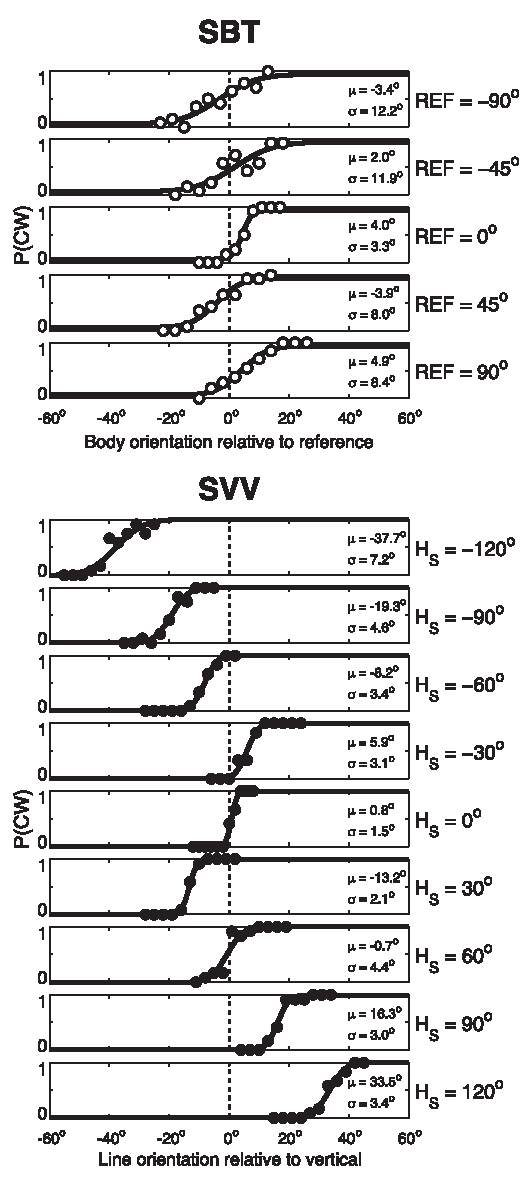
\includegraphics[width=0.5\textwidth]{src/paper1/figure3.pdf}
    
    \caption{SBT versus SVV performance in one subject (S1). Top, SBT. Proportion of CW responses is plotted against body orientation relative to the reference orientation (0\textdegree, \textpm45\textdegree, or \textpm90\textdegree). $\mu > 0\degree$ indicates tilt underestimation. Bottom, SVV. Proportion of CW responses is plotted against line orientation relative to vertical. Solid lines, Best-fit cumulative Gaussians, typified by $\mu$ and $\sigma$.}  
    \label{p1:fig3}
\end{figure}

The bottom section of Figure 3 illustrates the performance of the same subject in the SVV task. Each panel demonstrates how the fraction of CW responses changes as a function of line orientation relative to the perceived vertical, for each tilt angle tested. Performance is very accurate in the upright condition. For moderate body tilts, i.e., 30∞, this subject shows small systematic errors, indicating that the line must be set in a direction opposite to the head tilt to be perceived vertical in space. For larger tilts (=60∞), systematic errors occur with increasing tilt angle, with amplitudes up to 40\textdegree, as if tilt is underestimated. This response pattern is consistent with previous literature \cite{aubert1861, udodehaes1970, mittelstaedt1983, vanbeuzekom2000}. Close scrutiny also reveals that the precision in the vertical percept deteriorates away from the upright position. 

Psychometric fits capture these observations. In the upright position, the percept of visual vertical is virtually unbiased, as indicated by a µ value of 0.8∞. At large tilts, e.g., at -120\textdegree and 120\textdegree, $\mu = -37.7\degree$ and $\mu = 33.5\degree$, respectively, which means that the line must be tilted away from true vertical to be perceived as vertical in space. Furthermore, the fitted psychometric curves are steepest at 0\textdegree tilt, reflected by $\sigma = 1.5\degree$. With larger tilt angles, $\sigma$ increases, reaching maximum values of 7.2\textdegree and 4.3\textdegree at tilts of -120\textdegree and +120\textdegree, respectively. 

The results of this subject are exemplary for all subjects, as shown by the bias and SD data points in Figure 4. The mean results across the seven subjects are shown in the rightmost column. The bold lines in Figure 4 represent the fits from our Bayesian model, which will be discussed later in this section. 

\begin{figure}
	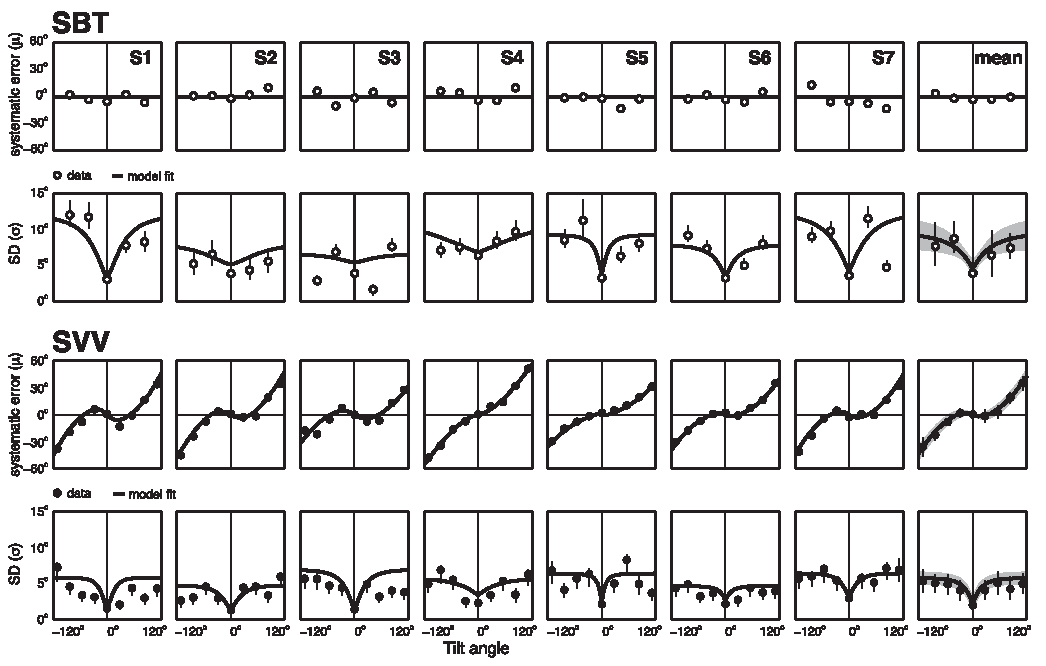
\includegraphics[width=1.0\textwidth]{src/paper1/figure4.pdf}
	
    \caption{Model predictions superimposed on parameters from the psychometric fits to the SBT (two top rows) and SVV data (two bottom rows). Accuracy and variability characteristics as a function of roll-tilt angle are shown; values are psychometric fits ($\mu$ and $\sigma$ values, [CIRCLES]) and model predictions (line) from all subjects. Mean data and mean predictions across subjects are plotted in the rightmost column.}
    \label{p1:fig4}
\end{figure}

The two top rows in Figure 4 show the accuracy ($\mu$) and precision ($\sigma$) of SBT percepts, now plotted against body orientation. For each subject, these values ($\mu$ and $\sigma$) were derived from the fitted cumulative Gaussian curves (Fig. 3). Biases for SBT, shown in the top row of Figure 4, indicate moderate deviations in either direction from perfect performance, but no systematic pattern emerges. Across the seven subjects, the $\mu$ values ranged from -14.2\textdegree to +11.7\textdegree across the five SBT tasks. On average, however, there was no systematic bias for the five body orientations (ANOVA; F(4,24) = 1.4; p = 0.25), as also indicated by the rightmost panels. The data further show that, in all subjects, variability is statistically lower ($p < 0.05$) at the upright orientation, with s values <4∞, than in the tilted conditions (45\textdegree and 90\textdegree), with $\sigma$ values ranging up to ~12∞. 

The two bottom rows of Figure 4 summarize our SVV data across the entire tilt range. Accuracy is close to perfect at upright orientation in all subjects, with mean values ranging between 0.1∞ and 2.8∞. For tilts =60∞, all subjects show systematic SVV errors (biases) of undercompensation, ranging up to maximum values close to 60∞. Three subjects (S1, S2, and S3) also show slight errors of overcompensation in the smallest tilt range (<60∞). The variability in the SVV is <3.0∞ for upright, which is consistently lower than in the tilted conditions, where variability reaches values ranging up to 8∞. 

Together, the results in Figure 4 show that SVV and SBT have different accuracy and precision characteristics. Subjects perceive their body-tilt angle more accurately than the spatial orientation of the visual line. However, when it comes to variability, performance is reversed: SVV curves are narrower than the SBT curves in all subjects, at both tilt angles, meaning that they are consistently less variable in the SVV task than in the SBT task. 

\subsection{Model predictions}

The bold lines in Figure \ref{p1:fig4} present the predictions of the Bayesian integration model, fitted simultaneously to the original responses from the SBT and SVV tasks. The rightmost column of Figure \ref{p1:fig4} shows the mean predictions from this model superimposed on the averaged parameters from the psychometric fits, indicating that the sensory integration model can account very well for all the characteristics of the data. 

By design (see Materials and Methods), the sensory integration model fits a horizontal fit line through µSBT = 0∞ because it cannot account for the small systematic SBT errors. As to SBT precision, the model predictions show an increase of noise with tilt angle similar to the actual increase of noise between 0∞ and 90∞ tilt, for all subjects. These model fits further suggest that the increase of SBT noise is steepest at small tilt angles and levels off at larger tilts. According to the model, the increase of SBT noise with tilt angle is attributable to the corresponding increase of noise in the head sensors (parameter aHS), but levels off by the constant noise level in the body sensors. The third row in Figure 4 depicts the model predictions of the systematic SVV errors, which show a very good match. Also with respect to SVV variability, fits and data show similar trends, suggesting an increase of SVV noise with tilt angle, which levels off at larger tilts. 

For each subject, best-fit parameter values and their bootstrap-based SD levels are listed in Table \ref{p1:tab1}. Parameter bHS, representing the noise (sHS) in the otolith signal in the upright subject, ranges between 1.1∞ and 3.9∞. Best-fit values of parameter aHS are significantly positive (p < 0.05) for all subjects, ranging from 0.07∞/∞ (S4) to 0.23∞/∞ (S1). This implies that the noise in the otoliths increases with tilt angle. The width of the head-in-space prior (sHSP) ranges from 9.4∞ (S2) to 18.7∞ (S5), with a mean of 12.5 ± 3.2∞, consistent with our previous report \cite{devrijer2009}. Best-fit values of parameter sBS, reflecting the noise in the sensory body-in-space signal, range from 6.7∞ (S3) to 15.0∞ (S5), with a mean of 10.8 ± 3.1∞, which is about twice as large as the best-fit values of parameter sHB, reflecting noise in the head-on-body signal, ranging from 1.8∞ (S6) to 9.3∞ (S3), with a mean of 4.9 ± 2.7∞. Thus, the parameter fits imply that the neck sensors are more precise than the body-tilt sensors. As has been discussed extensively in our previous paper \cite{devrijer2009}, the amplitude of uncompensated ocular counterroll (AOCR) shows large intersubject variability. 

\begin{table}

\begin{tabular}{lllllll}
\hline
Subject & $a_{HS}$ (\textdegree/\textdegree) & $b_{HS}$ (\textdegree) & $\sigma_{HSP}$ (\textdegree) & $\sigma_{BS}$ (\textdegree) & $\sigma_{HB}$ (\textdegree) & $A_{OCR}$ (\textdegree) \\
\hline
S1 & 0.23 \textpm 0.02 & 1.2 \textpm 0.32 & 11.6 \textpm 1.0 & 12.3 \textpm 1.1 & 3.3 \textpm 1.2 & 27.0 \textpm 2.2 \\
S2 & 0.12 \textpm 0.02 & 1.2 \textpm 0.52 & 9.4 \textpm 1.1 & 8.4 \textpm 2.9 & 6.4 \textpm 4.1 & 17.0 \textpm 3.8 \\
S3 & 0.20 \textpm 0.03 & 1.1 \textpm 0.42 & 14.4 \textpm 1.7 & 6.7 \textpm 1.9 & 9.3 \textpm 2.4 & 17.5 \textpm 2.1 \\
S4 & 0.07 \textpm 0.50 & 3.9 \textpm n/a & 11.2 \textpm 1.3 & 12.6 \textpm 2.3 & 7.1 \textpm 3.5 & 0 \textpm n/a \\
S5 & 0.11 \textpm n/a & 3.3 \textpm 1.0 & 18.7 \textpm 4.8 & 15.0 \textpm n/a & 3.6 \textpm 2.1 & 1.06 \textpm n/a \\
S6 & 0.23 \textpm 0.09 & 3.0 \textpm 1.5 & 9.5 \textpm 1.1 & 8.0 \textpm 0.83 & 1.8 \textpm n/a & 18.8 \textpm 4.1 \\
S7 & 0.20 \textpm 0.14 & 3.2 \textpm 1.0 & 12.8 \textpm 2.4 & 12.7 \textpm 6.1 & 3.0 \textpm n/a & 20.8 \textpm 9.0 \\
Mean & 0.16 \textpm 0.06 & 2.4 \textpm 1.2 & 12.5 \textpm 3.2 & 10.8 \textpm 3.1 & 4.9 \textpm 2.7 & 14.6 \textpm 10.2 \\
\hline
\multicolumn{7}{l}{Imposed fit limits were as follows: $a_{HS}$: 0.5\textdegree/\textdegree; $b_{HS}$, $\sigma_{HSP}$, $\sigma_{BS}$, $\sigma_{HB}$, 50\textdegree; $A_{OCR}$, 30\textdegree. SD values are not shown (n/a) when bootstrapped values formed a skewed distribution. $a_{HS}$, Tilt-related increase in otolith noise; $b_{HS}$, otolith noise in upright position; $\sigma{HSP}$, width of head-tilt prior; $\sigma{BS}$, noise in body-in-space sensors; $\sigma{HB}$, noise in neck sensors; $A_{OCR}$, uncompensated ocular counterroll.} \\
\end{tabular}

\caption{Best-fit parameter and bootstrap-based SD values}
\label{p1:tab1}
\end{table}

\subsection{Sensory weights}
 
To obtain the model fits in Figure \ref{p1:fig4}, we made the assumption (see Introduction) that information from both direct and indirect pathways (Fig. \ref{p1:fig1}) is used to estimate body and head orientation in space. The sensory weights, indicating the relative contribution of both pathways, can be computed from the fit results in Table 1. To obtain the body-in-space estimate, necessary for the SBT, the model uses both direct information from the body sensors and indirect information from the combination of otolith and neck information. Because the variability of the otolith signal (sHS) increases with tilt angle (aHS > 0), as shown in Table 1, the relative importance of direct and indirect pathways becomes dependent on tilt angle. This can be seen in Figure 5(top row), which shows the relative weights of these signals for each subject, derived from Equation 2 and the best-fit parameter values in Table 1. The mean (±SD) pattern across subjects is shown in the rightmost pattern. 

\begin{figure}
    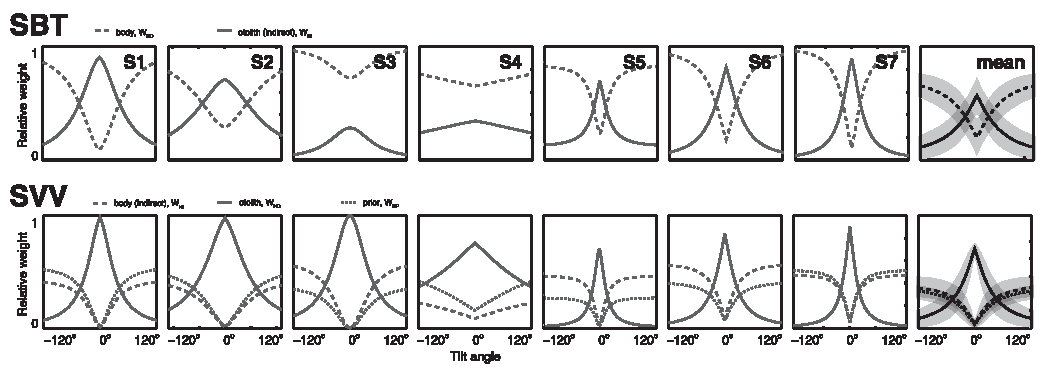
\includegraphics[width=1.0\textwidth]{src/paper1/figure5.pdf}
    
    \caption{Tilt dependence of weight factors in SBT (top) and SVV (bottom) for each subject. Trends with tilt angle are similar for all subjects. Head-in-space prior is only involved in SVV computations. Means across subjects are plotted in the rightmost column.}
\end{figure}

Instead of an overall dominance of body receptors in the direct pathway, the model implies that it is actually the indirect pathway, carrying the otolith signal, that dominates the behaviorally important range near upright. In most of our subjects (S1, S3, S5, S6, and S7), it was only when the otoliths became less reliable, at larger tilts, that the body sensors (direct pathway) got the upper hand (wBD > 0.5). 

For the SVV task, the model assumes that both information from the otoliths (direct) and the combination of body and neck information (indirect) is used. Figure 5 (bottom row) illustrates the relative contributions from these sensors as well as from the prior, based on the model fits (Table 1) and Equation 6. The SVV pattern looks similar to the SBT pattern (Fig. 5, top row): in all subjects, the otoliths are very dominant near upright, with weights close to 1, but their contribution declines when tilt angle increases. As we saw for the SBT signal weights, this decline reflects increasing otolith noise levels. In the SVV, the decline is steeper than in the SBT, where the reference frame transformation leads to an enhanced noise level with a less pronounced tilt dependence. As the otolith contribution decays, the contributions of the prior and indirect pathway become more manifest. According to our model fits, the weight of the body sensors in the SVV task (wHI) at 90∞ tilt ranges between 0.19 (S4) and 0.53 (S6). 

\subsection{Model evaluation}
 
To test whether the assumption of indirect pathways in the model is warranted, we compared its performance with a reduced version with only direct pathways (see Materials and Methods). With this in mind, we performed a likelihood ratio test of the complete model fit (with direct and indirect pathways) versus the fit of a model with direct pathways only [i.e., SVV just based on head sensors (the otoliths), the SBT just based on body sensors]. The results are shown in Table 2. For each subject, the complete model provided a significantly better account of the data than the reduced model without multisensory integration through the indirect pathways. In other words, head, neck and body sensors all contribute to both SBT and SVV. 

\begin{table}
\begin{tabular}{llllll}
\hline
Subject & MLE full model & MLE reduced model & $p$ & BIC full model & BIC psychometric fits \\
\hline
S1 & 231.5 & 312.4 & \textless 0.001 & 498.1 & 540.3 \\
S2 & 197.8 & 216.9 & \textless 0.001 & 430.6 & 539.3 \\
S3 & 267.5 & 313.4 & \textless 0.001 & 570.0 & 548.2 \\
S4 & 207.5 & 218.2 & \textless 0.001 & 450.0 & 569.1 \\
S5 & 195.6 & 216.3 & \textless 0.001 & 426.2 & 571.0 \\
S6 & 163.5 & 183.2 & \textless 0.001 & 362.0 & 502.5 \\
S7 & 248.0 & 260.0 & \textless 0.001 & 531.1 & 633.5 \\ 
\hline
\multicolumn{6}{l}{Log-likelihood ratio test of the full model (with indirect pathways) and reduced model (without indirect pathways). For all subjects, the full model outperforms the reduced model lacking multisensory integration through the indirect pathways. BIC values are much lower for the Bayesian integration model compared with separate psychometric fits in six of seven subjects.} \\
\end{tabular}
\caption{Validation of the model}
\label{p1:tab2}
\end{table}


We also compared our model, which provides a mechanistic explanation of the full dataset, with the pure descriptive account of the data as obtained by fitting separate psychometric curves to the data for the five SBT angles and nine SVV angles (Eq. \ref{p1:eqn1}, Fig. \ref{p1:fig3}, and \nameref{p1:sec:methods}, Model evaluation). Maximum-likelihood estimates were calculated and corrected for the number of free parameters using the BIC. As shown in Table 2, we found the lowest BIC values, indicating a better model, for the Bayesian model in all subjects, except S3. One might argue that the mean corrections before fitting the Bayesian model added another nine parameters that should be taken into account when comparing the models, even though these parameters were not fitted by the model. However, even for the worst-case scenario of 16 parameters, our Bayesian model still outperformed the individual psychometric fits (BICmechanistic = 3583 < BICpsychometric = 3910). 

\subsection{Model validation}
 
To further validate the model, we independently tested one of its predictions that can be assessed experimentally in isolation: head-on-body variance. In supine position, subjects judged their head orientation (CW/CCW) relative to the body midline after it had been passively roll-rotated with speeds subthreshold for the canals to various angles (see \nameref{sec:methods}, Model validation: independent test of neck noise). Psychometric fits indicate no systematic bias in these head-on-body percepts (data not shown). Figure 6 depicts the experimental noise levels derived from these psychometric fits and the predicted values provided by the model, including their 95\% confidence intervals. Because the variance of the estimates increases with the average head-on-body percept, we performed a regression on the log-transformed data \cite{hopkins2000}. The significant correlation between predicted and measured neck noise levels (slope, 1.03; intercept, -0.1; p = 0.04) provides an independent confirmation of the proposed model. 

%\begin{figure}
\begin{wrapfigure}{l}[5pt]{0.5\textwidth}
    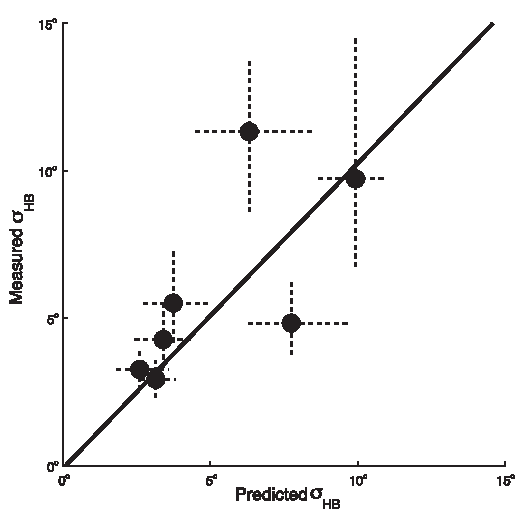
\includegraphics[width=0.5\textwidth]{src/paper1/figure6.pdf}
%\end{figure}
\end{wrapfigure}
\section{Discussion}

In this study, we made intrasubject comparisons of the accuracy (bias) and precision (inverse variance) characteristics in two spatial orientation tasks: SBT and SVV. The main experimental findings were as follows: (1) the SBT is more accurate than the SVV, (2) the SBT is less precise than the SVV, and (3) both SBT and SVV precision are smaller in tilted conditions than near upright. Under the assumption of optimality, a Bayesian model of sensory integration could account very well for these findings. Independent measurements, in supine subjects, of head-on-body variance confirmed the predicted value. 


\subsection{Comparison with previous work}
 
A world-vertical visual line appears tilted in space when the head is tilted in a darkened room (Aubert, 1861). Mittelstaedt (1983) was the first to emphasize that this phenomenon cannot be explained by errors in the body-tilt percept. He showed that subjects could accurately adjust themselves to a horizontal position, but, once in this position, made substantial systematic errors in the perception of visual verticality. Later, combined tests confirmed the discrepancy between SVV and SBT accuracy \cite{mast1996, jarchow1999, vanbeuzekom2000, vanbeuzekom2001, kaptein2004, vingerhoets2008}. The present study is consistent with these findings, showing substantial systematic SVV errors at tilts =60∞ and fairly accurate SBT performance. 

Compared with the abundant literature on SBT and SVV accuracy, data on their perceptual variability are scarce. In contrast to Mittelstaedt's observation (1983), Mast and Jarchow (1996) found that the SBT was much more variable than the SVV. The present study, the first to measure both SVV and SBT precision using an extensive psychometric approach, has clearly established that SBT variability is consistently higher than SVV variability, both in the upright and in the horizontal (90∞) tilt position. 

Furthermore, although various studies have noted that SVV variability increased at larger tilts \cite{schone1964, schone1968, udodehaes1970, vanbeuzekom2001, devrijer2008}, little is known about SBT variability as a function of tilt angle. Nelson (1968) showed that subjects were more variable when adjusting themselves to a horizontal position than to a vertical (upright) position. The present findings are consistent with these early observations. 


\subsection{Implications of the model}
 
After earlier indications that both the otoliths and body sensors contribute to the SBT (e.g., Clark and Graybiel, 1963, 1964; Nelson, 1968), Mittelstaedt (1997) made a quantitative assessment of their impact, using an ingeniously designed experiment. Subjects lay on their side in a horizontal centrifuge. The crux of the experiment was to vary the distance between the rotation axis and the interaural axis to equalize the opposite contributions from the otoliths and the body sensors so that the subject felt horizontal. By testing normal, paraplegic, and nephrectomized subjects, Mittelstaedt inferred how much each sensory system contributes to body-tilt perception. It was shown that, apart from the otoliths, also internal ``graviceptors'' in the trunk (such as the viscera) participate in the computation of the SBT. Later, some related studies provided evidence that the distribution of blood in the body also affects postural perception \cite{vaitl1997, vaitl2002}. According to Mittelstaedt (1998), the weight of the somatic graviceptors to estimate horizontal body orientation in healthy subjects is ~0.6 on average, with considerable intersubject variability. His estimate seems quite compatible with our wBD values at 90∞ tilt, which range between 0.35 (S5) and 0.93 (S6) (Fig. 5). 

Previous attempts to identify the separate contributions of the otoliths, neck, and body sensors on the SVV have yielded mixed results. Whereas Mittelstaedt (1998) found no evidence that the SVV was affected by the body sensors in his centrifuge experiment, other studies indicate that neck- and trunk-tilt aftereffects \cite{wade1968}, neck muscle vibration \cite{mckenna2004}, and manipulation of tactile and interoceptive body cues \cite{trousselard2004} can affect the SVV. In other words, even in the absence of direct head-in-space information from the otoliths, the brain can still obtain an estimate of head orientation in space through the indirect sensory pathway. These findings suggest that these modalities operate together with the otoliths in the computation of the SVV, consistent with our model. 


\subsection{Model evaluation}
 
The architecture of the model, as far as the reference frame transformations and the sensory integration is concerned, follows entirely from the principles of Bayesian inference. However, to account for our major findings and intersubject differences, we made two less straightforward assumptions. First, to explain the increased variability in both tasks at 90∞ tilt, we allowed for the possibility that the otoliths become more noisy with increases in tilt. Second, we hypothesized that prior knowledge is used in the visual vertical but not in body-tilt perception. Can these assumptions be justified on physiological and rational grounds? 

One reason to assume that otolith noise depends on tilt angle is based on the fact that the utricle contains considerably more hair cells than the saccule \cite{rosenhall1972, rosenhall1974}. Because the utricle is most sensitive to tilts of ~0∞, whereas the saccule is most sensitive at ~90∞ tilt \cite{jaeger2008}, this may well cause the proposed increase of otolith noise with tilt angle (Tarnutzer et al., 2010). A tilt-dependent noise level of the otoliths would also help to explain why the perturbing effect of roll-optokinetic stimulation on the SVV \cite{dichgans1974, fernandez1976} and on the SBT \cite{young1975} is more pronounced at larger tilt angles and why the SVV is more strongly influenced by residual canal signals at larger tilt angles, after prolonged roll rotations \cite{lorincz2008}.

In the SVV literature, it is widely assumed that the visual vertical is determined by a weighted combination of a sensory head-tilt signal and a head-fixed reference, denoted as the idiotropic vector \cite{mittelstaedt1983}. Recently, this idiotropic vector has been reinterpreted in terms of a Bayesian prior \cite{eggert1998, macneilage2007, devrijer2008}, with which it is mathematically equivalent. Interestingly, when tested in gravity-free conditions, subjects still retain a sense of visual vertical, always aligned with their long-body axis, compatible with the idea of head-fixed prior \cite{mittelstaedt1983}. Vingerhoets et al. (2008) recently found a similar phenomenon in the SVV during multiple-cycle dynamic roll rotation in normal gravity. Remarkably, when the same subjects were tested in a comparable dynamic SBT experiment, their responses showed very little bias on average, indicating that a prior is used only in the SVV and not for body-tilt estimation. To explain how this difference in computational approach might make sense, Vingerhoets et al. (2008) speculated that precision is more important than accuracy for the visual system, for reasons of visual stability. Combining the sensory tilt signal with prior knowledge yields a more stable percept of visual space than can be derived from the sensory signal alone. In a recent study, Bortolami et al. (2006) report virtually no bias in the haptically indicated vertical, which would be consistent with the suggestion that the prior plays primarily a role in visual processing. Likewise, for body-tilt perception, for which it might be less important to be precise and more useful to be accurate, the prior does not take part in this process. 

\subsection{Clinical implications}
 
According to our model, statistically optimal performance requires the use of information from both direct and indirect pathways to estimate body and head orientation in space (Fig. 1). Thus, if one of the sensory inputs is lost or severely disrupted, SBT and SVV performance will deteriorate, but should not completely break down due to their multimodality dependence. By setting the appropriate parameter values of the model to infinity, we simulated the model to predict SVV and SBT performance in two patient groups: bilateral vestibular patients (noise level of the otoliths set to infinity) and patients with somatosensory loss (noise level of the body sensors set to infinity). Figure 7 shows the results of these simulations. 

%\begin{figure}
\begin{wrapfigure}{l}[5pt]{0.5\textwidth}
    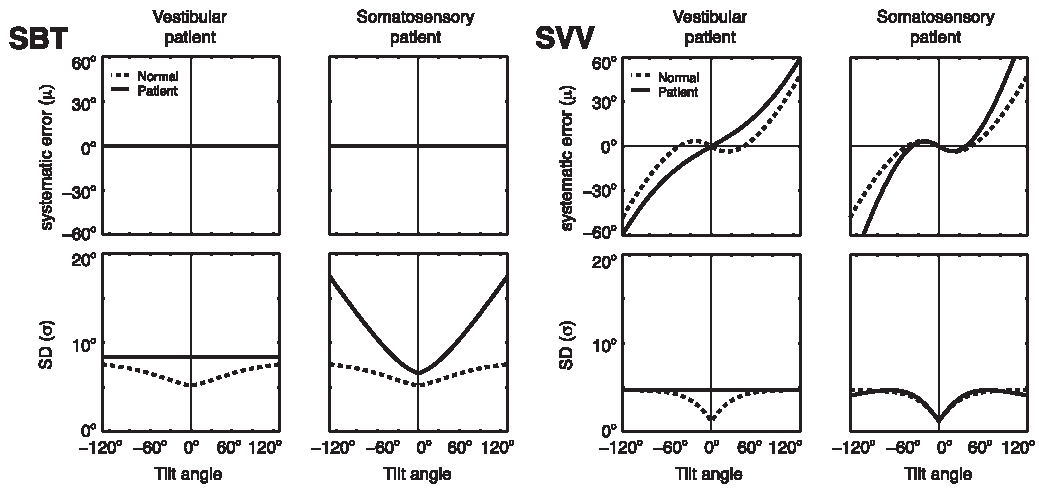
\includegraphics[width=0.5\textwidth]{src/paper1/figure7.pdf}
\end{wrapfigure}
%\end{figure}

When the otolith signal is lost (vestibular patient), the model predicts increased but constant noise levels in both the SBT and SVV, regardless of tilt angle. From the perspective of our model, the increased SBT variability can be attributed to the loss of the otolith contribution through the indirect body-in-space pathway. The increased bias in the SVV, predicted by the model, can also be understood: as the sensory-derived head-tilt estimate becomes noisier, the effect of the prior becomes more noticeable. Although there are no accuracy and variance measurements across the entire tilt range in these patients, the few previously published deficits are consistent with these predictions. Bisdorff et al. (1996) have shown that bilateral vestibular patients performed quite accurately in the SBT at upright, but were ~40\% more variable than normal subjects. Bronstein et al. (1996) showed that vestibular patients still compensated for their tilt angle when testing the SVV at 90∞, but with a bias about twice as large as in normal subjects, consistent with our simulations. 

The right column of Figure 7 depicts a simulation of the SBT and SVV in a patient with loss of somatosensory information (somatosensory patient). In this case, the SBT depends solely on otolith information mediated through the indirect pathway. Although this signal is still accurate, it is spoiled by the larger variability of the neck signal, needed to perform the appropriate reference frame transformation. The model also predicts larger errors in the SVV in these patients than in normal subjects. Although there are no reports containing measurements of bias and variance in the SBT and SVV, paraplegic patients show that along with the otoliths, internal body sensors also contribute to the SBT if lesions are below the 12th thoracic segment \cite{mittelstaedt1997}. This evidence supports the design of our model. 

In conclusion, we have tested the performance of healthy subjects in two psychophysical tasks that probe two spatial orientation estimates---SBT and SVV---and show that perceptual accuracy and precision in these tasks can be linked to the reference-frame-dependent weighting of sensory signals. We verified our theoretical framework by independent measurements of neck noise levels and by showing that it can account for the stereotypical performance of two patient groups. In this respect, our reverse-engineering approach also provides a new tool to establish diagnostic and prognostic markers of the quality of the signals involved in spatial orientation in neurological disease. 

\section{Appendix}

Here we provide further explanation about the Bayesian computations underlying the SVV as expressed in Equations 6 and 10 in Materials and Methods. Figure 8 illustrates graphically that the variance of the posterior distribution in a single trial (sH~S2) is not simply the same as the variance in its peak location in multiple trials, s2(H~S). In a single trial (Fig. 8A-C), the optimal estimate of head tilt is based on the likelihood (Fig. 8B, green curve) associated with the combined sensory input from the direct and the indirect pathway (Fig. 8A, green line, HS) and the prior (Fig. 8B, blue curve), by multiplication of the two probability distributions. The prior distribution is a Gaussian with mean HSP and variance sHSP2. The peak of the resulting posterior distribution (Fig. 8B, orange curve) is used as the optimal estimate of head tilt (H~S), given by the following: 

% Equation 13
\begin{equation}
\label{p1eqn13}
\tilde{H}_S = w_{HS} \cdot \hat{H}_S + w_{HP} \cdot H_{SP},
\end{equation}

with

% Equation 14
\begin{equation}
\label{p1eqn14}
w_{HS} = \frac{1 / \sigma^2_{HS}}{1 / \sigma^2_{HS} + 1 / \sigma^2_{HSP}},
\end{equation}

and

% Equation 15
\begin{equation}
\label{p1eqn15}
w_{HP} = \frac{1 / \sigma^2_{HSP}}{1 / \sigma^2_{HS} + 1 / \sigma^2_{HSP}},
\end{equation}

in which sHS denotes the noise in the sensory signal, known to the observer, and wHS and wHP represent the relative weights of the sensory signal and the prior, respectively. Note that Equation 13 is equivalent to Equation 1 in Materials and Methods. The variance of the posterior distribution in a single trial is given by the following: 

% Equation 16
\begin{equation}
\label{p1eqn16}
\sigma^2_{HS} = w_{HS} \cdot \sigma^2_{HS} \\
              = \frac{\sigma^2_{HSP}}{\sigma^2_{HS} + \sigma^2_{HSP}} \cdot \sigma^2_{HS}
\end{equation}

and is reflected by the width of the orange curve in Figure 8B. Figure 8D-F illustrates performance in multiple trials, in which the posterior distributions vary due to sensory noise (sHS), whereas the prior remains fixed. The variance of each posterior distribution is fixed and is given by Equation 16. 

%\begin{figure}
\begin{wrapfigure}{l}[5pt]{0.75\textwidth}
    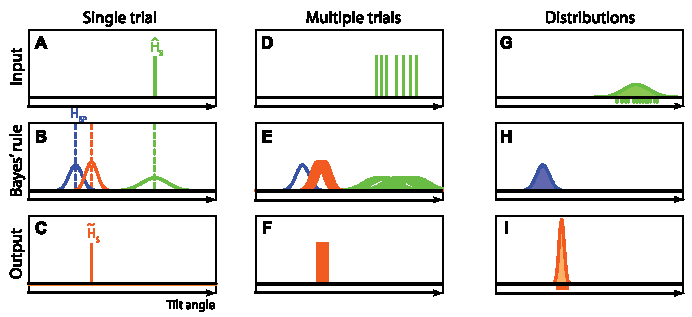
\includegraphics[width=0.75\textwidth]{src/paper1/figure8.pdf}
%\end{figure}
\end{wrapfigure}

That the variance of the peak locations across multiple trials, $\sigma^2(\tilde{H}_S)$, is smaller can be shown by applying the rules of noise propagation to Equation 13. 

% Equation 17
\begin{equation}
\label{p1eqn17}
\sigma^2(\tilde{H}_S) = \\
	\big( \frac{\delta\tilde{H}_S}{\delta\hat{H}_S^2} \big) \cdot \\
	\sigma^2(\hat{H}_S) + \\
	\big( \frac{\delta\tilde{H}_S}{\delta H_{SP}^2} \big) \cdot \\
	\sigma^2(H_{SP}) \\
	= w^2_{HS} \cdot \sigma^2_{HS} \\
	= \frac{\sigma^2_{HSP}}{\sigma^2_{HS} + \sigma^2_{HSP}} \cdot \sigma^2_{HS}
\end{equation}

which is equivalent to Equation 10 in Materials and Methods. Corresponding panels G-I (Fig. 8) illustrate the distribution of the sensory signals for a given tilt angle (green-shaded curve), the prior distribution (blue-shaded curve), and the optimal estimates (orange-shaded curve), respectively. Figure 8I illustrates that the distribution of the optimal estimates across many trials has a lower variance than the posterior distribution in each single trial (Fig. 8B), which follows from the comparison of Equations 16 and 17, respectively. 



\bibliography{refs}{}

\titleformat{\chapter}
{\normalfont\Large\bfseries}{\thechapter}{0.2em}{}
\titlespacing*{\chapter}{0pt}{-30pt}{10pt}

\end{document}

\documentclass[10pt,b5paper,twoside]{book}


%
% Common packages and custom commands used by the main .tex files.
%

\usepackage[dutch,british]{babel}
\usepackage[nottoc]{tocbibind}
\usepackage{multicol}
\usepackage{amsmath}
\usepackage{amsfonts}
\usepackage{amssymb}
\usepackage{graphicx}
\usepackage{gensymb}
\usepackage{textcomp}
\usepackage{hyperref}
\usepackage{doi}
\usepackage{xcolor}
\usepackage{nameref}
\usepackage{xspace}
\usepackage{titlesec}
\usepackage{floatrow}
\usepackage{longtable}
\usepackage{siunitx}
\usepackage[outercaption]{sidecap}
%\usepackage{fancyhdr}
\usepackage{wrapfig}
\usepackage{lmodern}
\usepackage{multicol}
\usepackage[font={scriptsize, sf}, labelfont={sf,scriptsize,bf}]{caption}
\usepackage{src/apacite_custom}
\usepackage{src/thesis}



\pagestyle{plain}

\floatsetup[table]{font={scriptsize, sf}}

\hypersetup{colorlinks=true, linkcolor=blue, citecolor=blue}
\setcounter{tocdepth}{2}

% Do not add extra vertical space
\raggedbottom

% Indent paragraphs
\setlength{\parindent}{1.0cm}

\bibliographystyle{apacite_custom}

\renewcommand{\baselinestretch}{1.2}
\setlength{\parskip}{0ex plus 0.3ex minus 0.3ex}

\newcommand{\about}{$\approx$}

%% For the Chapter title, etc.
\newcommand{\bigrule}{\titlerule[0.5mm]}
\titleformat{\chapter}[display]
{\normalfont\filleft\bfseries\itshape}
{%
 \vskip-3em
\titlerule[1pt]%
\vspace{1pt}%
\titlerule
\vspace{1pc}%
\Large\MakeUppercase{\chaptertitlename} \thechapter}
{1pc}
{\titlerule
\vspace{1pc}%
\thispagestyle{empty}
\Huge}


\makeatletter
\renewenvironment{thebibliography}[1]
     {\footnotesize\begin{multicols}{2}[\chapter{\refname}]%
      \@mkboth{\MakeUppercase\refname}{\MakeUppercase\refname}%
      \list{\@biblabel{\@arabic\c@enumiv}}%
           {\settowidth\labelwidth{\@biblabel{#1}}%
            \leftmargin\labelwidth
            \advance\leftmargin\labelsep
            \@openbib@code
            \usecounter{enumiv}%
            \let\p@enumiv\@empty
            \renewcommand\theenumiv{\@arabic\c@enumiv}}%
      \sloppy
      \clubpenalty4000
      \@clubpenalty \clubpenalty
      \widowpenalty4000%
      \sfcode`\.\@m}
     {\def\@noitemerr
       {\@latex@warning{Empty `thebibliography' environment}}%
      \endlist\end{multicols}}
\makeatother


\hypersetup{
    pdfauthor = {Ivar Clemens, Luc Selen, Mathieu Koppen, and Pieter Medendorp},
    pdftitle = {Visual stability across combined eye and body motion}
}

\begin{document}

\selectlanguage{british}

\thispagestyle{empty}

\chapter{Visual stability across combined eye and body motion}
\chaptermark{}


\newpage

\small {\bf Abstract} In order to maintain visual stability during self-motion, the brain needs to update any ego-centric spatial representations of the environment. Here, we use a novel psychophysical approach to investigate how, and to which extent, the brain integrates visual, extraocular, and vestibular signals pertaining to this spatial update. Participants were oscillated sideways at a frequency of 0.63 Hz while keeping gaze fixed on a stationary light. When the motion direction changed, a reference target was shown either in front or behind the fixation point. At the next reversal, half a cycle later, we tested updating of this reference location by asking participants to judge whether a briefly flashed probe was shown to the left or right of the memorized target. We show that updating is not only biased, but that the direction and magnitude of this bias depend on both gaze and object location, implying that a gaze-centered reference frame is involved. Using geometric modeling, we further show that the gaze-dependent errors can be caused by an underestimation of translation amplitude, by a bias of visually perceived objects towards the fovea (i.e., a foveal bias), or by a combination of both.

\vfill

\noindent\underline{ \hspace{4cm} }

\noindent This chapter has been published as \newline
\noindent {\bf Clemens, I.A.H.}, Selen, L.P.J., Koppen, M. and Medendorp, W.P. \citeyear{clemens2012}. Visual stability across combined eye and body motion. \emph{Journal of Vision}, 12(12):8 1-11. \newline

\newpage


\section{Introduction}

A typical characteristic of human vision is that the position of the retina is constantly changing due to eye, head, and/or body movements. Yet, even during such self-motion, we retain a sense of whether visual objects are stable or moving with respect to an earth-centric reference frame \cite<see e.g.>{wallach1987}. This capability is essential for a correct percept of the world and the maintenance of visual stability.

Achieving visual stability is a complex process because visual signals are coded with respect to gaze, and not in an earth-fixed reference frame. When the visual scene lacks earth-centric landmarks, the brain should distinguish which changes in retinal input result from real world movement and which from eye movement. The usual view, dating back to Von Helmholtz \citeyear{vonhelmholtz1867}, is that this is achieved by subtracting the extraretinal signal of eye motion from the retinal image shifts \cite{wexler2005}.

Visual stability experiments in which participants made head-fixed saccades suggest that efference copies of the outgoing motor commands serve this purpose. Neurons in the frontal eye fields and the lateral intraparietal area demonstrate pre-saccadic shifts of receptive fields, elicited by an efference copy \cite{duhamel1992, kusunoki2003}. These gaze-centered shifts could allow the brain to anticipate and cancel out the changes in retinal input due to the saccade \cite{sommer2006}. Also, fMRI studies have reported evidence for shifting receptive fields in the human brain \cite{medendorp2003a}. 

Despite these important insights, head-fixed saccades are only one of a multitude of movements that are made in real life. Bringing the body in motion, like when driving a car, puts severe challenges on the mechanism underlying visual stability. In this case, when the body is translated passively, vestibular feedback informs the brain about the motion. This information must be combined with efference copies of orbital eye movements to interpret the changes in retinal input. Solving this problem is geometrically complicated because, during eye and body motion, the changes in retinal input depend nonlinearly on the depth and direction of objects that make up the retinal image, as in motion parallax \cite{medendorp2003b}.

Recent studies have reported fairly accurate reach or gaze responses to memorized target locations, presented prior to whole-body translations \cite<see for review:>{klier2008, medendorp2011}. However, such studies do not map one-to-one to the mechanisms of visual stability. First, the requirement of a motor response may invoke different processing mechanisms, which may be subject to different constraints. Second, motor response studies probe the system after the limb or eye movement, thereby revealing the combined result of all intervening spatial computations and transformations needed to guide the action.

In the present study, we investigate visual stability across simultaneous eye and whole-body motion without involving the motor system. To this end, we used a two-alternative forced choice (2-AFC) psychophysical approach in combination with a visual updating paradigm. Participants had to retain object locations during sinusoidal whole-body motion, while keeping their gaze fixed on a world stationary point either in front of or behind the object.

By systematically manipulating the parameters of retinal and extraretinal signals related to body translation, binocular fixation, and object location, we test how the brain integrates these signals for the maintenance of visual stability. Our results show consistent errors in visual stability, which strongly depend on the location of the object relative to gaze. Using a modeling approach, we explore possible causes underlying these gaze-centered updating errors.


\section{Methods}
\label{p2:sec:methods}

\subsection{Participants}

Eight participants (4 male, 4 female), aged between 22 and 41 years, provided written informed consent to participate in the experiment. All participants were free of any known vestibular or neurological disorder and had normal or corrected-to-normal visual acuity. Three participants (the authors) were knowledgeable about the purpose of the experiment, but their results did not differ from the five na\"ive subjects. Participants never received any feedback about their performance.

\subsection{Setup}

A linear sled on a 800mm track was used to laterally translate participants. The sled, powered by a linear motor (TB15N, Technotion, Almelo, The Netherlands), was controlled by a Kollmorgen S700 (Danaher, Washington DC, USA) drive. The kinematics of the sled were controlled with an accuracy better than 34 $\mu$m, 2 mm/s, and 150 mm/$\text{s}^2$. The sled was configured such that participants were seated on the sled with the interaural axis aligned with the motion axis. Participants were restrained using a 5-point seat belt and a chin rest. In addition, the head was firmly held in place using an ear-fixed mold.  Emergency buttons at both sides of the sled chair enabled subjects to stop the sled motion immediately if needed. Eye movements were recorded using an EyeLink II (SR Research, Kanata, Canada) eye tracking system. Its camera system, which was mounted to the sled, remained stable with respect to the head during the entire experiment. Eye positions were calibrated based on the visual fixations during the experiment, under the assumption that these fixations were accurate.

\subsection{Visual stimuli}

Participants had to memorize the location of a earth-centric visual target (reference, $R$) during half a period of sinusoidal body translation. We tested the quality of this memory by asking them to judge and report the position of a probe stimulus ($P$) relative to that memorized location, following a psychophysical procedure. The reference and probe stimuli were both presented using a one-dimensional 450mm wide array, consisting of 180 red light emitting diodes (LEDs), with a spatial separation of 2.5 mm between neighboring LEDs. The LED array was oriented in parallel with the motion direction of the sled, centered w.r.t. the sled's trajectory and at the same vertical level as the participant's eyes. It was positioned with an accuracy better than 5 mm, at one of five different distances (850, 1050, 1200, 1400, or 2070 mm) from the participant's eyes in front of the sled. We further positioned an LED at either 850, 1050, 1200, 1400, or 2070 mm in front of the participant, on a virtual line orthogonal to the sled's motion direction and crossing the center of the LED array. These latter LEDs served as earth-stationary gaze fixation points ($FP$) during the experiment, so that gaze was directed either behind or in front of the stimulus array. The fixation points were displaced vertically by a few mm, such that the fixation point and the LED array did not occlude each other.

\subsection{Paradigm}

The experiments employed a paradigm that studies the constancy of spatial locations during 0.63 Hz sinusoidal whole-body motion in the lateral direction (left-right motion). We tested the effects of body translation (T, 150 or 300 mm peak-to-peak amplitude), fixation depth ($FP$, four spatial locations), and depth of the reference target ($R$, four spatial locations) on the quality of perceptual stability. These quantitative data will be interpreted using the geometric framework outlined in the subsection \nameref{p2:sec:model} below.

\begin{figure}
	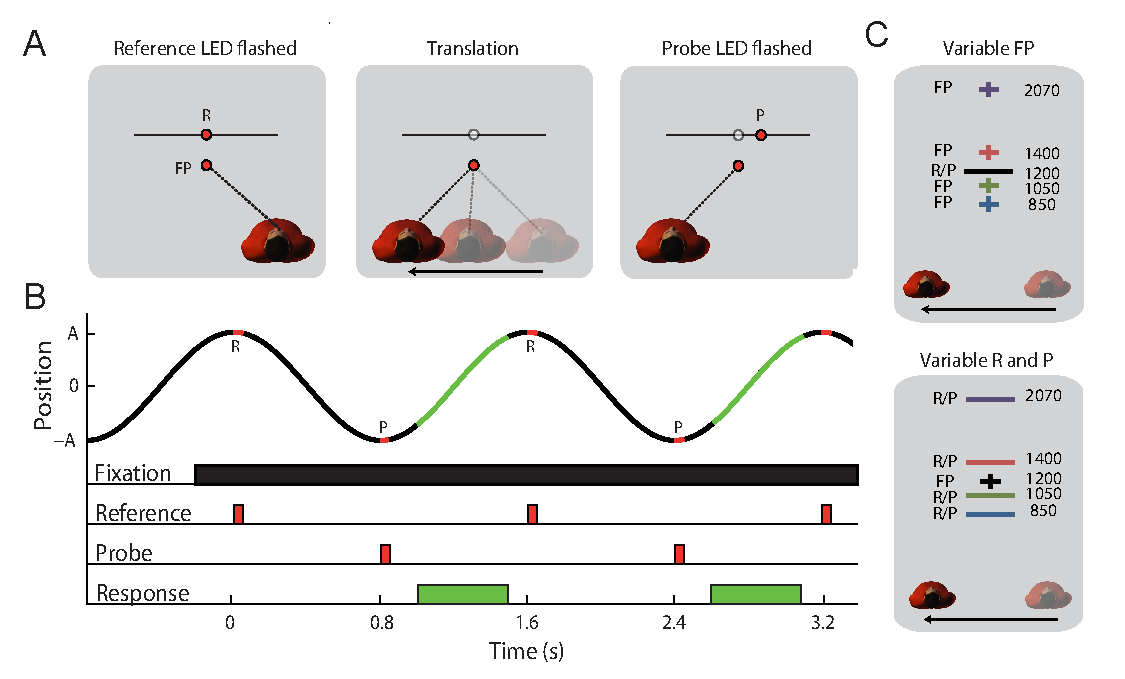
\includegraphics[width=1.0\textwidth]{src/paper2/figure1.pdf}
	
	\caption{(A) Top-view illustrating three key events within the experiment. Left panel: At the extreme right position, the reference target (R) is flashed. Middle panel: The participant moves while keeping fixation on the fixation point (FP). Right panel: At the left most position, one of the probe locations (P) is flashed. (B) Timing of key events. Within a run of sinusoidal sled motion, participants always fixated the fixation point. At the rightmost point, the reference (R) was flashed for 50 ms. Then, at the extreme left position, a probe (P) was shown for 50 ms. Participants responded whether the probe was presented to the left or right of the reference using a joystick. (C) Locations of fixation points (plus signs) and reference/probe locations (bars) used in our experiment (see also Table \ref{p2:tab1}).}
	
	\label{p2:fig1}
\end{figure}

Figure \ref{p2:fig1}, panels A and B, illustrate the paradigm in detail; Figure \ref{p2:fig1}C provides an overview of the experimental conditions. The experiment consisted of runs of either 30 or 15 trials. Each run started with the onset of a FP, to be fixated for the entire duration of the run. To avoid discontinuous acceleration at motion onset, sled velocity was linearly increased over one sinusoidal cycle (see Merfeld, Park, Gianna-Poulin, Black, and Wood, 2005 for a similar approach). Once the steady-state sinusoidal motion was reached, participants were tested using a visual updating task (Figure \ref{p2:fig1}A). More specifically, at the most rightward position, when the body motion reversed direction, the reference R (here, the center LED) was presented for 50 ms. When the sled reached the left-most position, again during motion reversal, the participant's estimate for the location of R was tested by displaying another LED, the probe P, for 50 ms. The participant then had to report the location of this probe relative to R in a two-alternative forced choice (leftward, rightward) using a joystick. While we asked participants to respond in a timely manner, we did not explicitly constrain response time. Therefore, the next trial was only presented after a response was given. In practice, most responses were given within half a cycle (RT {\textpm}SD = 0.59s \textpm0.09, across participants). We used an adaptive algorithm to vary the spatial separation between reference and probe target from trial to trial \cite{kontsevich1999}, mapping out psychometrically the bias and precision of visual stability across whole-body motion. 

Participants were tested in 16 conditions, each comprising a unique combination of translation amplitude (T), visual fixation point (FP), and reference (R) position (see Fig \ref{p2:fig1}C). The values used in this experiment are shown in Table \ref{p2:tab1}. For each condition we presented 135 trials, which were divided into 4 runs of 30 trials and one run of 15 trials. In every condition 70 out of 135 trials were normal trials, that is, the central LED was used as reference. The other 65 trials in each condition were catch trials, of which 25 trials had the reference location shifted 36 mm to the left of the central led; another 25 had the reference location 36 mm rightward, and in 15 trials a random LED in the stimulus array was taken as the reference location. The catch trials were to prevent participants from simply making repeated stereotypic responses. After each run, the lights were turned on. Following a 30 s break, the experiment resumed automatically. The total experiment was divided into three sessions, tested on different days.  Each participant was tested on a total of 2160 trials.

\begin{table}    
    \begin{tabular}{lll}
    $FP$ (mm) & $R/P$ & $T$ (mm) \\
    \hline
    1200 & 850 & 75 and 150 \\
    1200 & 1050 & 75 and 150 \\
    1200 & 1400 & 75 and 150 \\
    1200 & 2070 & 75 and 150 \\
    850 & 1200 & 75 and 150 \\    
    1050 & 1200 & 75 and 150 \\
    1400 & 1200 & 75 and 150 \\
    2070 & 1200 & 75 and 150 \\
    \end{tabular}
    
    \caption{Fixation distance (FP), distance to reference and probe targets (R/P) and translation amplitude for each of the 16 unique visual updating conditions.}
    
    \label{p2:tab1}
\end{table}

\subsection{Data analysis}

To prevent effects caused by vergence and/or version eye-movements, we excluded trials in which participants did not maintain fixation within a 3 degree interval around FP, during the time interval starting 100ms before presenting the reference target and ending 100ms after cueing the probe. Overall, 6.4\% \textpm1.7\% ({\textpm}SD) of all trials were discarded per participant based on these eye movement criteria. 

For each condition, we quantified performance by calculating the probability of a rightward response as a function of the location of the probe relative to reference location. We used a maximum likelihood fit of a cumulative Gaussian function to summarize the psychometric data:

\begin{equation}
\label{p2:eq1}
P(x) = \lambda + (1 - 2\lambda) \frac{1}{\sigma \sqrt{2\pi}} \int_{-\infty}^{x}{e^{-(y-\mu)^2 / 2\sigma^2}}dy,
\end{equation}

in which x represents the size of probe displacement. The mean of the Gaussian, $\mu$, represents the bias in visual stability (positive $\mu$ corresponding to a rightward bias). The width of the curve, corresponding to the standard deviation $\sigma$ of the Gaussian, is inversely related to precision, and serves as a measure of the participant's variability in the visual updating task. Parameter $\lambda$, representing the lapse rate, accounts for stimulus-independent errors caused by subject lapses or mistakes and was restricted to small values ($\lambda < 0.06$). Fits were performed using the 'psignifit' Matlab toolbox \cite{wichmann2001, wichmann2001b}.


\subsection{Model}
\label{p2:sec:model}

We investigated whether the observed bias can be explained by allowing a gain factor in the processing of the lateral translation by the vestibular system. That is, we assume that $\tilde{T} = {\alpha}T$, where $\tilde{T}$ is the perceived and $T$ the actual translation \cite{medendorp1999}. If the spatial update is performed entirely in a head-centered system, the effect of this gain would be straightforward. The reference flash $R$ is presented when the sled is in the rightmost position and the following translation of the sled by $T$ mm to the left in world coordinates amounts to a translation of the world, including the reference point, by $T$ mm to the right in head-coordinates. Due to the gain of the vestibular system the perceived translation equals ${\alpha}T$ mm to the right, leading to a predicted bias of

\begin{equation}
\label{p2:eq2}
\mu = \tilde{T} - T = (\alpha - 1) T
\end{equation}

in mm on the LED array. Thus, when processed in a head-centered system, the bias would be negative for $\alpha < 1$, positive for $\alpha > 1$; it would be proportional to the translation amplitude, but would not depend at all on the reference and fixation point positions.
Previous experiments \cite{vanpelt2007} have shown that reach targets are updated not in head-centered coordinates, but rather within a gaze-dependent frame of reference. Following up on this, we also model the effect of the translation gain in a gaze-centered system. Let OF be the vector from the cyclopean eye to the fixation point and, similarly, $OR$ the vector to the reference point. The translation by $T$ mm to the left in world coordinates is in head-coordinates well approximated by a rotation of OF by $T/|OF|$ radians to the right and a rotation of OR by $T/|OR|$ radians to the right. (The approximation is good, since both $T<<|OF|$ and $T<<|OR|$. To express the gist of the prediction of the gaze-dependent model, this first-order approximation is very useful; in the actual calculations the precise geometry was used, without noticeable differences.)  Consequently, in gaze-centered coordinates (i.e., OF fixed straight ahead) the vector OR rotates by an angle of 

\begin{equation}
\label{p2:eq3}
\phi \approx T (\frac{1}{|OR|} - \frac{1}{|OF|})
\end{equation}

radians to the right. In modeling the perceived rotation angle $\tilde{\phi}$ we again replace $T$ by $\tilde{T} = {\alpha}T$, but we also have to consider possible biases in the perception of $|OR|$ and $|OF|$. Following previous literature \cite{gogel1977, medendorp2003b}, we assume that the depth of the constantly visible fixation point is perceived accurately, i.e., $|\tilde{OF}| = |OF|$, but we allow that the perceived depth of the 50 ms flashed reference stimulus, $|\tilde{OR}|$, is biased towards this fixation point depth. Since the depth signals available in this experiment (vergence angle and disparity) express more directly in terms of inverse depth than depth itself. The simplest way to implement such a bias is to model the perceived reference depth as a weighted harmonic mean of the actual reference and fixation depths:

\begin{equation}
\label{p2:eq4}
\frac{1}{|\tilde{OR}|} = \beta \frac{1}{|OR|} + (1 - \beta) \frac{1}{|OF|}
\end{equation}

where $\beta = 1$ represents the limiting case of accurate depth perception of the reference stimulus (no bias) and $\beta = 0$ the limiting case of full "assimilation" to fixation point depth. In total this leads to a perceived rotation angle of

\begin{equation}
\label{p2:eq5}
\tilde{\phi} = {\alpha}T \cdot \beta(\frac{1}{|OR|} - \frac{1}{|OF|})
\end{equation}

radians to the right. Comparing Eq. \ref{p2:eq5} with Eq. \ref{p2:eq3} shows that our assumptions amount to a total gain of $\alpha\beta$ on the rotation angle, with freely interchangeable contributions of the parameters $\alpha$ and $\beta$. We substitute $\gamma = \alpha\beta$ and note that the resulting bias in angle, $\tilde{\phi} - \phi$, is observed as a bias in mm on the LED array at a distance $|OR|$:

\begin{equation}
\label{p2:eq6}
\mu = (\tilde{\phi} - \phi)|OR| = (\gamma - 1)T(1 - \frac{|OR|}{|OF|})
\end{equation}

Thus, in the gaze-centered model the bias is again proportional to translation amplitude, but now it also depends critically on the fixation and reference point positions. In particular, the bias flips sign according to presenting the reference point in front of or behind the fixation point. On top of this, there is an overall (across all conditions) sign dependence on the combined values of the translation gain and fixation depth bias factors.

\section{Results}

Participants were tested in an experimental paradigm that studies the stability of spatial locations across combined eye and body motion. The task, illustrated in Figure 1, requires that subjects fixate an earth-stationary central fixation point, FP, which is visible throughout the run. At two successive reversals of motion direction, at the right and left excursion point of the sinusoidal motion, a reference (R) and a probe (P) target are briefly flashed. In a two-alternative forced choice task, the participant has to indicate whether the probe location was to the left or to the right of the reference location. The resulting psychometric data provide a quantitative assessment of the bias ($\mu$) and precision ($\sigma^{-2}$) of visual stability across self-motion (see Methods for details). Depending on the stimulus conditions (FP, R, and T), participants may erroneously judge the location of R, and hence provide biased responses.

Figure \ref{p2:fig2} shows the results of a typical participant, plotting the fraction of rightward responses (indicated by the circles) as a function of horizontal probe location relative to the reference. The 16 conditions are split into 4 panels according to the manipulated variable: FP distance (top panels), reference distance (bottom panels) and translation amplitude (left vs. right panels). Data for all individual probes are presented (circles). In an ideal observer, all psychometric functions would constitute a step response centered at zero, indicating no bias and no uncertainty. However, the actual data show consistent biases and non-zero variance.

When FP was behind R, we observed a leftward bias (top panels; red and purple curves), that increased when fixation was further away from the reference location (red vs. purple dots). When FP was in front of R (green and blue dots), the opposite pattern was seen. Furthermore, as T increases, psychometric curves move away from zero (t-test; $t(63) = -4.55$, $p < 0.05$) and become less steep (t-test; $t(63) = -4.64$, $p < 0.05$), a sign that there is decay in both accuracy and precision (compare left and right panels). Similar biases are observed when keeping FP constant, and varying the location of R, as demonstrated by the bottom panels. We derived estimates of the bias ($\mu$) and corresponding standard deviation ($\sigma$) values in each of the 16 conditions, for all subjects.

\begin{figure}
    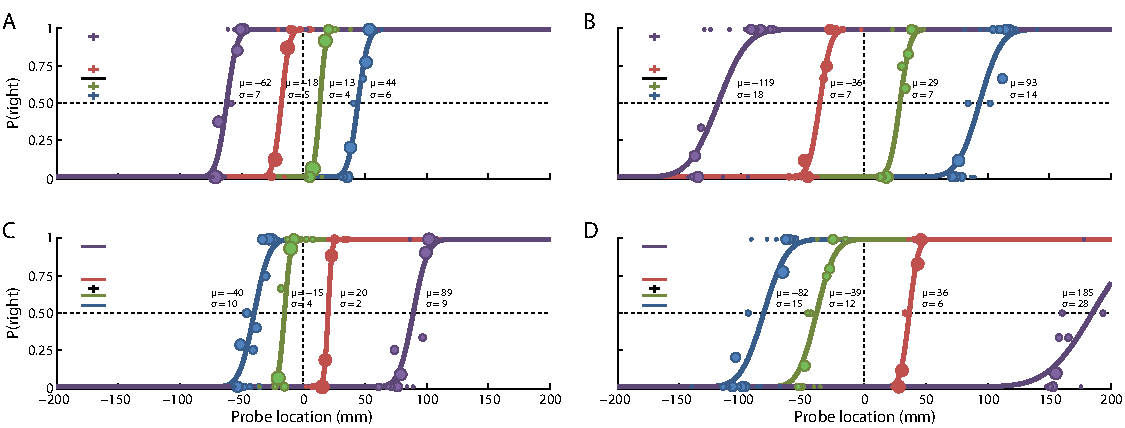
\includegraphics[width=1.0\textwidth]{src/paper2/figure2.pdf}
    
    \caption{Performance in one subject (S1). The proportion of rightward responses is plotted against probe location relative to the reference. Size of a data point represents the number of trials tested. Solid lines, best-fit cumulative Gaussians, characterized by bias (l) and standard deviation (r). (A) Constant reference depth, variable fixation depth, 150 mm translation. (B) Constant reference depth, variable fixation depth, 300 mm translation. (C) Variable reference depth, constant fixation depth, 150 mm translation. (D) Variable reference depth, constant fixation depth, 300 mm translation.}
    
    \label{p2:fig2}
\end{figure}

Figure \ref{p2:fig3} depicts the bias ($\mu$) for each subject (dots), together with the mean bias {\textpm}SD across subjects (error bars), in top-view panels. This shows that the pattern in Figure \ref{p2:fig2} holds across all participants, with biases ranging between -126 and 212 mm. Clearly, the bias in updating of the central target increases with T and depends on FP, reversing for gaze fixation behind versus in front of the R (two top panels). Likewise, when FP was kept constant, the updating bias is not only larger for the larger T, but also depends on the location of R, with the bias in opposite directions for targets presented in front versus behind fixation (two bottom panels). Taken together, these observations suggest that the location of R relative to gaze, rather than the head-centric locations of FP or R, is a crucial factor in determining the updating bias. 

\begin{figure}
    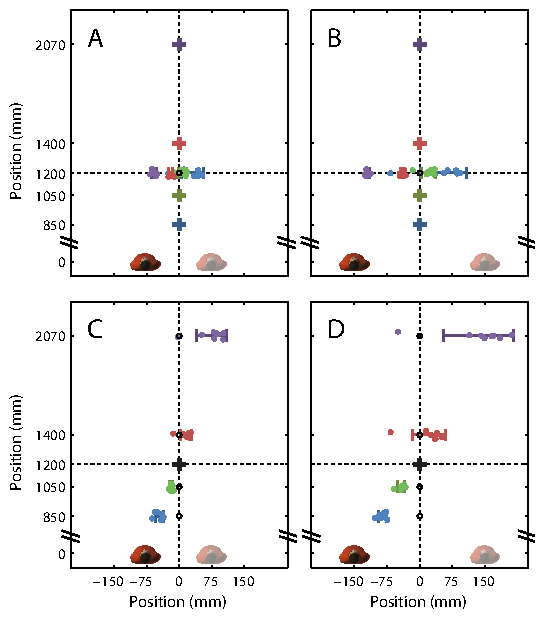
\includegraphics[width=0.75\textwidth]{src/paper2/figure3.pdf}
    
    \caption{Top view of the updating biases ($\mu$). Dots, individual bias values; error bars, averages (\textpm SD) across participants; +, fixation point. (A), (B), (C), (D): Conditions as in Figure \ref{p2:fig2}.}
    
    \label{p2:fig3}
\end{figure}

To further analyze these observations, Figure 4 plots the bias values ({\textpm}SE across participants) as a function of gaze fixation FP (panel A), target location R (panel B) and reference location relative to gaze fixation FP - R (panel C). Both the location of FP and R, as well as the bias are expressed in units of degrees instead of millimeters because the former is more closely associated with native visual coordinates. (In practice, however, because of the large distance, visual angles are about proportional to the associated horizontal distances). While in panel A no clear relationship is observed ($R^2 = 0.09$, $F(1,14) = 1.32$; $p > 0.05$), panel B reveals only a weak linear relationship ($R^2 = 0.25$, $F(1,14) = 4.71$; $p < 0.05$). However, in panel C the data for all conditions are rearranged such that they fall into a single response curve. A linear fit shows a very strong correlation in this case ($R^2 = 0.97$, $F(1,14) = 483$, $p < 0.05$). This suggests that the observed errors almost solely depend on the location of R relative to gaze.

\begin{figure}
    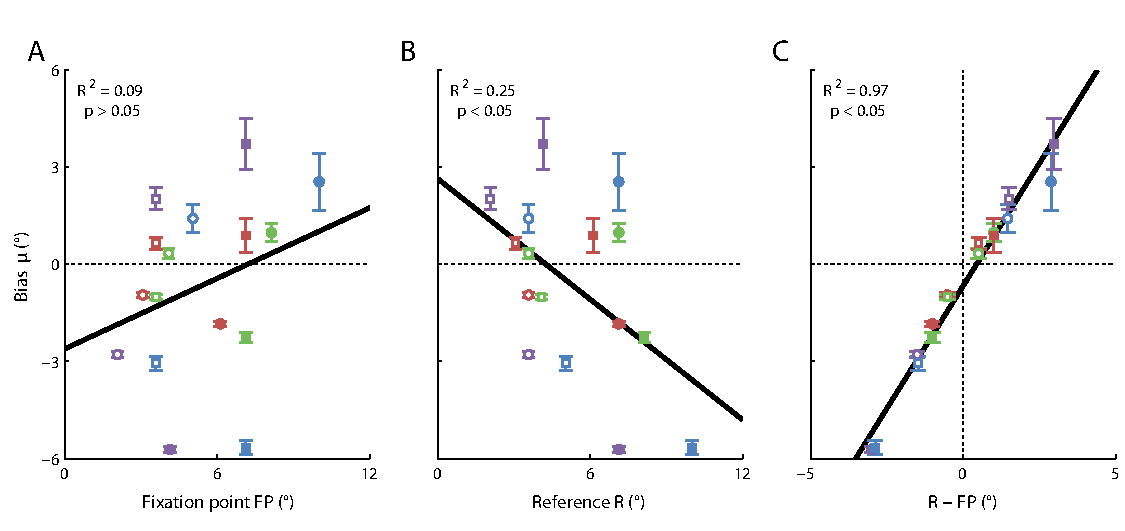
\includegraphics[width=1.0\textwidth]{src/paper2/figure4.pdf}
    
    \caption{Head- versus gaze-centered effects in updating bias (l). (A) Average bias (6 SE) across participants plotted against head- centric version angle of fixation point, for each of the 16 conditions. (B) Same data plotted as a function of head-centric angle to the reference location. (C) Same data plotted against the gaze-centric location of the reference target. Open symbols, 150 mm translation. Closed symbols, 300 mm translation. Circles, constant fixation depth. Squares, constant reference depth. Color scheme as in Figure \ref{p2:fig1}C.}
    
    \label{p2:fig4}
\end{figure}

To validate this notion, we fit two different models to explain the updating biases: a head- and gaze-centered model (see Eqs. \ref{p2:eq2} and \ref{p2:eq6} respectively, in \nameref{p2:sec:methods}). Because the updating bias systematically depends on gaze, we expect the gaze-centered model to outperform the head-centered model. Indeed, the RMSE of the gaze-centered model was significantly lower (t-test; $t(7) = -3.68$, $p < 0.05$) than that of the head-centered model. Table \ref{p2:tab2} presents the RMSE values for both models and the fit-results of the gaze-centered model for each participant. According to this latter model, the best-fit value of the gain $\gamma$ (mean 0.25 \textpm0.08 SE) is considerably lower than the ideal value of one. In the Discussion we will address the possible implications of this small value.

\begin{table}
    \begin{tabular}{llll}
    & Head-centered & FIX & ME \\
    Participant & RMSE (\textdegree) & $\gamma$ & RMSE (\textdegree) \\
    \hline
    1 & 0.32 & 0.13 & 0.06 \\
    2 & 0.29 & 0.17 & 0.05 \\
    3 & 0.13 & 0.81 & 0.23 \\
    4 & 0.64 & 0.29 & 0.59 \\
    5 & 0.31 & 0.14 & 0.07 \\
    6 & 0.31 & 0.16 & 0.11 \\
    7 & 0.28 & 0.23 & 0.07 \\
    8 & 0.33 & 0.07 & 0.10 \\
    \end{tabular}

    \caption{RMSE values for both models and best-fit values for the gaze-centered model parameter ($\gamma$, Equation \ref{p2:eq6}).}

    \label{p2:tab2}
\end{table}

Finally, in addition to accuracy, we also quantified the precision of the updated R. Figure 5 shows the standard deviation ($\sigma$ {\textpm}SE across participants) of the psychometric functions as a function of either FP (panel A), the head-centered location of R (panel B) or the gaze-centered location of R (panel C), in the same format as Fig. 4. No significant effects can be observed in panels A and B ($R^2 = 0.18$, $F(1,14) = 3.14$, $p > 0.05$ and $R^2 = 0.00$, $F(1,14) = 0.03$, $p > 0.05$ respectively). Panel C shows a significant linear relationship ($R^2 = 0.41$, $F(1,14) = 9.68$, $p < 0.05$). From this, we conclude that precision decreases for targets that are further or nearer in depth relative to fixation, and therefore also more peripheral in gaze-coordinates.

\begin{figure}
    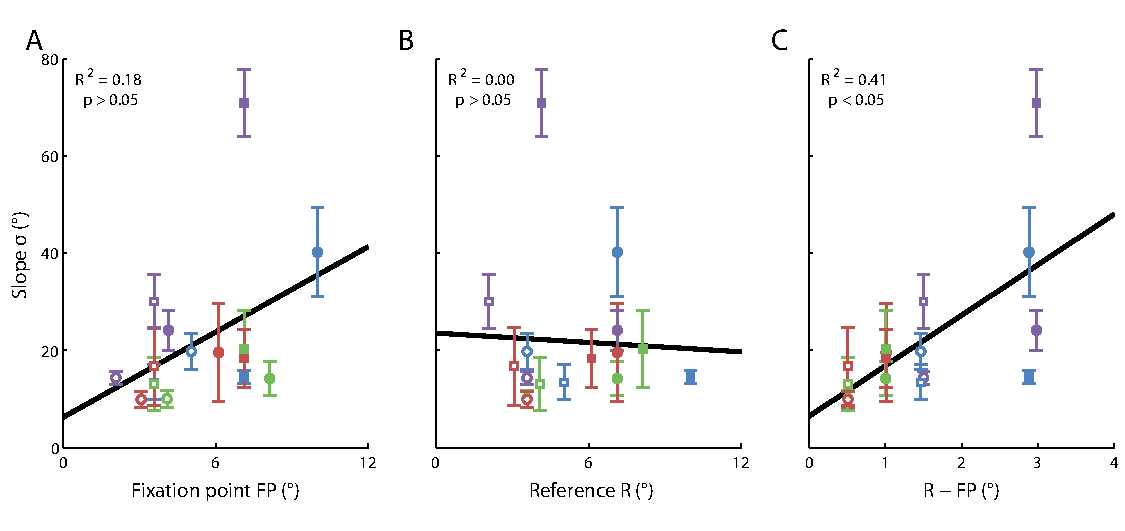
\includegraphics[width=1.0\textwidth]{src/paper2/figure5.pdf}
\end{figure}

\section{Discussion}

We investigated how the brain integrates retinal and extraretinal signals in order to maintain visual stability across combined eye and body motion. Participants had to remember the location of a world-fixed reference target, flashed in the periphery, while their body was passively translated and their binocular gaze actively changed in order to fixate a world-stationary target LED. When body motion reversed direction, a probe target was presented and the participant indicated whether it was shown to the left or right of the memorized reference. The resulting psychometric curves revealed substantial biases in the updating of the reference target, which increased with depth from fixation and reversed in sign for reference targets presented at opposite depths from fixation. In addition, precision of visual stability decreased when the distance between this target and the fixation point increased, likely due to the lower spatial resolution in the retinal periphery \cite{westheimer1982}. Geometric modeling suggests that these observations are consistent with spatial updating in a gaze-centered reference frame. In the following, we compare our results to previous work, and explore possible explanations of our observations in context of the gaze-dependent updating model.

\subsection{Relation to previous studies}

To our knowledge, there have been no other studies that have psychophysically investigated perceptual stability during combined eye and body motion. So far, related studies have tested spatial stability using paradigms in which participants make saccades or reaches to previously flashed targets after intervening self-motion (see Klier and Angelaki, 2008; Medendorp, 2011 for review). 
For actively generated self-motion, Medendorp et al. (2003b) had participants make saccade-vergence movements to remembered targets that were presented before they made a sidestep. Although their participants initially misperceived the targets, i.e. they underestimated the depths of distant targets and overestimated depths of near targets \cite{gogel1977, komoda1974, philbeck1997}, they accurately compensated for the intervening motion in the updating of the perceived target location, following the required non-linear updating patterns. Similar observations were made in relation to the updating of spatial locations across active self-motion for reaching \cite{admiraal2004, flanders1999, medendorp1999, vanpelt2007}. Compared to the present study, compensation for active intervening whole body motion was substantially better in all these studies.
Regarding passively induced self-motion, previous work by Isra\"el and Berthoz \nocite{israel1989} and more recent observations by Klier, Hess and Angelaki (2008) showed that human participants can also update the locations of saccade targets for passive whole body motion. Similar experiments in non-human primates have also demonstrated compensation for translational motion in the updating of saccadic space \cite{li2005a}. Although the amount of compensation depended on the depth of fixation, it was typically less than geometrically required (see their figure 4B), as in the present results. The same experiments were also conducted in labyrinthectomized monkeys, showing that their updating is even more compromised \cite{li2005b, wei2006}. This suggests that otolith information interacts with visual information to update saccade goals. 
Thus, in view of previous studies, our results are consistent with the notion that spatial ability is better maintained across active compared to passive body motion, perhaps due to the presence of efference copies of motor commands during active motion. Furthermore, based on the present findings it seems that perceptual updating is worse when compared to the action-oriented updating in previous studies. Should this be interpreted in favor of the proposal that visuospatial updating is organized in distinct processing pathways, one for conscious perception and one for the control of action \cite{goodale1992}? We do not want to suggest this. There may be other factors that contribute to the relatively low updating performance in the present study. Using geometric models (i.e., Eqs. 2 and 6) we will now explore such factors in more detail.

\subsection{Modeling implications}

In order to systematically explore possible explanations for the updating performance found in the present study, we now return to the head- and gaze-centered models of the updating mechanism presented in Eqs. 2 and 6 respectively. These models were inspired by the models proposed by Van Pelt and Medendorp (2007), with the addition of the possibility of a foveal bias. In the head-centered model (Eq. 2), the updating bias is proportional to the translation amplitude, but independent of reference and/or fixation point positions. However, since our data show a clear and systematic dependence on these positions (see Figs. 2-4), this model is not viable.
This leaves us with the gaze-centered model of Eq. 6, which incorporates these dependencies. Estimating the overall gain parameter ? in this gaze-centered model yielded a mean value of ? = 0.25 across participants. Since this ? is the product of parameters ? and ? (see Eq. 5), this entails that at least one of these parameters must be considerably smaller than one, the veridical value. That is, in the updating process the translation is perceived with a small gain (? << 1) and/or there is a distinct bias towards fixation depth (? << 1). We now explore the plausibility of these explanations in turn. 
For the perception of body translation at least two signals may be important: the vestibular signal from the otoliths and the changes in eye position while tracking the visual FP. Both linear acceleration (peak: 231 cm/s2) and frequency (0.63 Hz) were well above the detection thresholds of the otoliths \cite{benson1986, yu2012}. Furthermore, the firing rate of otolith afferents increases monotonically with acceleration in our frequency range \cite{fernandez1976, yu2012}, and can therefore be used to correctly decode acceleration. However, this does not mean that further processing of acceleration into a velocity or displacement signal is veridical \cite{merfeld2005}. In fact, it has been shown that the translational vestibuloocular reflex is not perfectly compensatory at the frequency that we have tested. However, when the vestibular signal is complemented by visual following mechanisms, participants are able to maintain fixation \cite{medendorp2002, paige1998}. This indicates that a near veridical percept of translation is possible by combining vestibular and eye position information. Yet, higher level processing of the translation signal might still be biased. For instance, the conversion of translated distance into an updating angle might be faulty, and/or the actual updating process itself could misinterpret an otherwise veridical updating angle. It has been shown that near-veridical updating takes place for e.g. reach targets \cite{henriques1998, vanpelt2007} where errors are attributed to the reference frame transformation instead. This suggests that the gaze-centered remapping process itself, which is thought to drive spatial updating, is not biased.
Thus, when considering previous work, it is most likely the higher level processing of the translation signal that governs the observed biases. One such processing step concerns the problem of attributing visual motion to either self-motion or object-motion \cite{vonhelmholtz1867}. If this attribution is flawed, it can have a profound influence on updating and might be the cause of our low updating gain. Support for this idea is found in work by Dyde and Harris (2008) who showed that participants make such attribution errors, in particular in conditions of passive translation and darkness, both of which apply to our study. In the active translation studies mentioned earlier, this effect is likely diminished by the presence of an efference copy that helps in disambiguating self-motion from object-motion.
A further explanation for our low overall gain is that depth perception of the reference point is biased (? << 1). Because the reference and probe lights were flashed for only 50ms at the zero velocity points of the sinusoidal motion and the head is unable to move relative to the body, depth perception of these lights is likely to be compromised. Actually, the spatial updating process that takes place in our experiment can alternatively be described in terms of a Bayesian model. To represent the brain's assumption that, lacking any precision information, the depth of peripheral stimuli is at or close to fixation point depth, such a model will involve a prior distribution centered at this fixation depth. The full specification of such a Bayesian model is beyond the scope of this paper. Here, we have opted for a more straightforward geometrical modeling approach (Eqs. 2 to 6), in which such a foveal depth bias appears in Eq. 4 with the weight 1 - ?. While such foveal influences have been reported previously \cite{brenner2008, mateeff1983}, for this to be the sole explanation for our low gain would require the foveal bias to be 80\%, which is quite extreme.
In conclusion, we have shown systematic biases in visual stability across combined eye and body movements. These biases are consistent with a gaze-centered updating model, with simple gain factors on both translation and depth perception.  



\bibliography{refs}{}

\titleformat{\chapter}
{\normalfont\Large\bfseries}{\thechapter}{0.2em}{}
\titlespacing*{\chapter}{0pt}{-30pt}{10pt}

\end{document}

\documentclass[10pt,b5paper,twoside]{book}


%
% Common packages and custom commands used by the main .tex files.
%

\usepackage[dutch,british]{babel}
\usepackage[nottoc]{tocbibind}
\usepackage{multicol}
\usepackage{amsmath}
\usepackage{amsfonts}
\usepackage{amssymb}
\usepackage{graphicx}
\usepackage{gensymb}
\usepackage{textcomp}
\usepackage{hyperref}
\usepackage{doi}
\usepackage{xcolor}
\usepackage{nameref}
\usepackage{xspace}
\usepackage{titlesec}
\usepackage{floatrow}
\usepackage{longtable}
\usepackage{siunitx}
\usepackage[outercaption]{sidecap}
%\usepackage{fancyhdr}
\usepackage{wrapfig}
\usepackage{lmodern}
\usepackage{multicol}
\usepackage[font={scriptsize, sf}, labelfont={sf,scriptsize,bf}]{caption}
\usepackage{src/apacite_custom}
\usepackage{src/thesis}



\pagestyle{plain}

\floatsetup[table]{font={scriptsize, sf}}

\hypersetup{colorlinks=true, linkcolor=blue, citecolor=blue}
\setcounter{tocdepth}{2}

% Do not add extra vertical space
\raggedbottom

% Indent paragraphs
\setlength{\parindent}{1.0cm}

\bibliographystyle{apacite_custom}

\renewcommand{\baselinestretch}{1.2}
\setlength{\parskip}{0ex plus 0.3ex minus 0.3ex}

\newcommand{\about}{$\approx$}

%% For the Chapter title, etc.
\newcommand{\bigrule}{\titlerule[0.5mm]}
\titleformat{\chapter}[display]
{\normalfont\filleft\bfseries\itshape}
{%
 \vskip-3em
\titlerule[1pt]%
\vspace{1pt}%
\titlerule
\vspace{1pc}%
\Large\MakeUppercase{\chaptertitlename} \thechapter}
{1pc}
{\titlerule
\vspace{1pc}%
\thispagestyle{empty}
\Huge}


\makeatletter
\renewenvironment{thebibliography}[1]
     {\footnotesize\begin{multicols}{2}[\chapter{\refname}]%
      \@mkboth{\MakeUppercase\refname}{\MakeUppercase\refname}%
      \list{\@biblabel{\@arabic\c@enumiv}}%
           {\settowidth\labelwidth{\@biblabel{#1}}%
            \leftmargin\labelwidth
            \advance\leftmargin\labelsep
            \@openbib@code
            \usecounter{enumiv}%
            \let\p@enumiv\@empty
            \renewcommand\theenumiv{\@arabic\c@enumiv}}%
      \sloppy
      \clubpenalty4000
      \@clubpenalty \clubpenalty
      \widowpenalty4000%
      \sfcode`\.\@m}
     {\def\@noitemerr
       {\@latex@warning{Empty `thebibliography' environment}}%
      \endlist\end{multicols}}
\makeatother


\hypersetup{
    pdfauthor = {Ivar Clemens},
    %pdftitle = {Choosing our words},
    %pdfsubject = {Language production},
    %pdfkeywords = {language production; }
}

\begin{document}

\selectlanguage{british}

\thispagestyle{empty}

\chapter{Integration of ocular and vestibular signals for self-motion perception in darkness}
\chaptermark{}

\newpage

\small {\bf Abstract} Self-motion is typically accompanied by compensatory eye movements that help minimize retinal slip and maximize dynamic visual acuity. To date, it is unknown whether these eye movements also have a reversed role, serving as a cue for self-motion perception. To address this question, we had participants ($n=8$) judge self-motion during different eye movement conditions in the absence of full-field optic flow.  In a 2-AFC task, participants indicated whether the second of two successive passive lateral whole-body translations was longer or shorter than the first. Eye movements during each translation were world-stationary, body-stationary in an otherwise dark room. Results of these two conditions show that the perceived translations were shorter with body-fixed gaze compared to world-fixed gaze. Using a linear model, we estimated the relative contributions of vestibular and eye movement signals to self-motion perception and found that eye movement signals contribute approximately 25 percent. The model was independently validated by successfully predicting the effects of eye movements on self-motion in a third condition without any visual fixation, i.e. when the eyes were free to move. We conclude that eye movement signals influence self-motion perception, even in the absence of visual stimulation, and even when oculomotor and vestibular estimates are in conflict, e.g. during body-fixed gaze. We hypothesize that adverse consequences of this seemingly inflexible arrangement are minimal under natural conditions because eye movements and self-motion are highly correlated, and because eye movements are most often accompanied by veridical optic flow cues to self-motion.

\vfill

\noindent\underline{ \hspace{4cm} }

\noindent This chapter is being prepared for publication \newline
\noindent {\bf Clemens, I.A.H.}, Selen, L.P.J., MacNeilage, P.R. and Medendorp, W.P. \citeyear{clemens2015a}. %Title. \emph{Journal}, volume(issue): from-to. \newline

\newpage

\section{Introduction}

An accurate estimate of self-motion is important to guide interactions with the environment. During passive self-motion both vestibular and optic flow signals provide information about self-motion \cite{gibson1955, benson1986, harris2000, israel1989, angelaki2005, carriot2013, chen2010}. However, also compensatory eye movements that maintain fixation on world-fixed objects carry self-motion information. These eye movements are driven by retinal slip or vestibular signals. For example, the linear vestibulo-ocular reflex (LVOR) stabilizes gaze during head translations, even in complete darkness \cite{paige1989,medendorp2002,angelaki2004}.  Many have shown that the brain uses oculomotor signals to extract the optic flow component related to self-motion \cite{warren1988, royden1992, freeman1998, lappe1999}, but to our knowledge a possible direct influence of eye movements on self-motion perception has not been investigated. Here we investigate whether these oculomotor signals are also used to estimate self-motion directly.

When gaze is world-stable during whole-body translation, the eye displacement correlates with translation size and is modulated by fixation depth \cite{schwarz1989, paige1998, mchenry2000, medendorp2002}. When properly scaled this eye movement signal could serve as a self-motion cue. In contrast, when fixation is body-fixed the eyes remain stationary in their orbits \cite{paige1998, ramat2005} making them no longer informative about self-motion. If, however, the brain assumes that eye movements are always made to maintain world-stable gaze, as in the LVOR, it would equate the absence of eye movements with the absence of self-motion. As a result, self-motion with body-fixed gaze should be underestimated compared to self-motion with world-fixed gaze, despite identical vestibular cues.

 This hypothesis implies that oculomotor signals are always combined with vestibular signals to estimate self-motion, even in complete darkness.  In this case, the size of the unconstrained eye movements should resemble a VOR movement that is intermediate between body- and world-fixed fixation, and should parametrically relate to the perceived self-motion.

To test whether eye movements are used in self-motion perception, we employed a two-alternative forced choice (2-AFC) paradigm in which participants were presented with two consecutive lateral translations. They had to indicate whether the second translation was longer or shorter than the first. Eye movements during each interval were either constrained using a  body or world stationary fixation point or not constrained at all (i.e. free). We show that identical translations were perceived shorter when gaze was body stationary compared to world stationary. Furthermore, using a linear model we predicted perceived displacement during the free gaze condition based on vestibular signals and unconstrained eye movements. We conclude that eye movements influence self-motion perception even in the absence of optic flow or other visual stimulation. 
\section{Materials and methods}
\label{p3:sec:methods}

\subsection{Participants}

Eight naive participants (three male, five female), aged between 22 and 29 years, provided written informed consent to participate in the experiment. All participants were free of any known vestibular or neurological disorder and had normal or corrected-to-normal visual acuity. Participants never received any feedback about their performance.

\subsection{Experimental setup}

A motorized linear sled \cite<see>[for details]{clemens2012} was used to laterally translate participants following a minimum jerk profile \cite{flash1985} of fixed duration (1 \si{\second}) and amplitudes ranging from 1 to 27 \si{\centi\metre}. Participants were seated on the sled such that the inter-aural axis aligned with the motion axis. They were restrained using a five-point seat belt and a chin rest. In addition, the head was held in place using a sled-fixed mold which resembled head-phones and pressed down on the head surrounding the pinnea . Auditory cues were suppressed using white noise presented through in-ear headphones. Experiments were conducted in complete darkness except for visual fixation points, projected by a laser pointer on a black bar 50 \si{\centi\metre} in front of the participant at eye level. Laser pointers used to project body-fixed targets were attached to the sled. Those used to project world-fixed targets were mounted on the wall behind the sled.

Eye movements were recorded at 500\si{\hertz} using an EyeLink II (SR Research, Kanata, Canada) system whose cameras were mounted to the sled and therefore remained stable with respect to the head during the entire experiment. Because the head and body positions were fixed during the experiment, the orientation of the eyes within the head, as measured by the tracker, was equivalent to the orientation of the eyes in space. The eye tracking system was calibrated before each session using 11 evenly spaced calibration points ranging from -22 to \siang{22} degrees. We used linear regression to link EyeLink measurements to gaze angles.

\subsection{Paradigm}
We used a two-alternative forced choice (2-AFC) task to measure perceived linear self-motion across three different eye fixation types: world-fixed, body-fixed, and unconstrained (free) fixation. We refer to these as world, body and free, respectively. A trial contained two sequential translation intervals of equal duration (1 \si{\second}) and in the same direction (either leftward or rightward). Different fixation types were presented in the two translation intervals. Participants were instructed to judge whether the translation during the second interval was longer or shorter compared to the first interval. They were additionally instructed to always look at the fixation point when it was visible; no instructions were given for when the fixation point was switched off (i.e. during free fixation).


\begin{figure}
    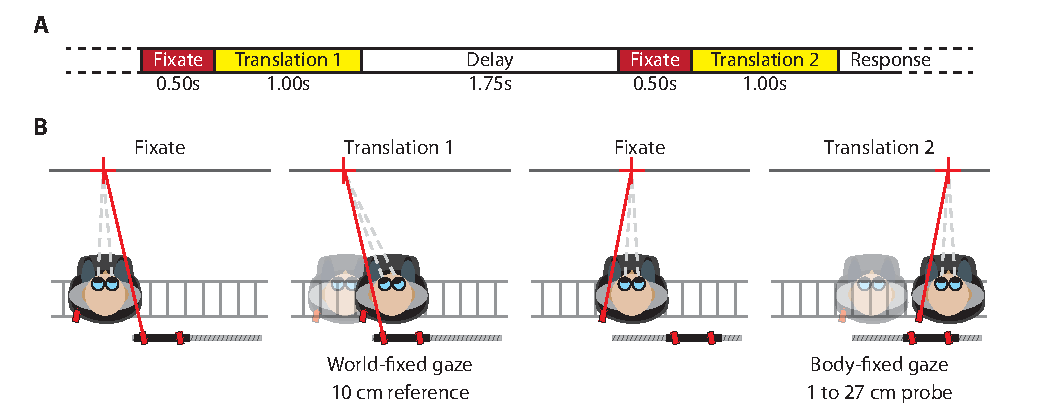
\includegraphics[width=1.0\textwidth]{src/paper3/figure1.pdf}

    \caption{\panelref{A} Time course of key events within a single trial. In each of the two intervals, a 0.50 \si{\second} fixation period (red) precedes the lateral translation (yellow). A 1.75 \si{\second} long delay period (shown in white) separates the two intervals. After the second translation, the participant responded whether this second translation was longer or shorter than the first. \panelref{B} Top-view illustrating key events during a body vs. world trial. First panel: participant fixates the world-fixed target (red cross) at the start of the first interval. Second panel: translation with world-fixed fixation target. Third panel: body-fixed fixation at start of second fixation interval. Fourth panel: translation with body-fixed fixation in second interval.}
    \label{p3:fig1}
\end{figure}

The time evolution of a single trial is shown in \figref{p3:fig1}. Each trial started with the onset of a central fixation point (i.e. aligned between the eyes) for 0.5 \si{\second}. Subsequently, the first translation interval commenced.  Depending on the fixation type, the fixation point remained visible (world and body) or was extinguished (free) during the translation interval. The trial shown in the figure depicts the 10 \si{\centi\metre} reference translation with world fixation. After this first interval, a delay followed in which the participant was kept in complete darkness for 1.75 \si{\second}. Then, the central fixation point reappeared, followed 0.5 \si{\second} later by the second interval, in which the probe translation was presented. The set of possible probe translations ranged from 1 to 27 \si{\centi\metre} in equidistant steps of 0.4 \si{\milli\metre}. The fixation type in the probe interval was always different than in the associated reference interval (the trial in \figref{p3:fig1} illustrates body fixation). After the second interval, the participant had to indicate whether he or she perceived the second translation as longer or shorter than the first using a 1-dimensional joystick. Moving the poke away from the body indicted that the second movement was longer, while moving it towards the body indicated that the second movement was shorter.


\begin{table}
    \begin{tabular}{llll}
    Comparison & Reference & 1st interval & Direction \\
    \hline
    Body vs. world & Body & Reference & Right \\
    & & & Left \\
    & & Probe & Right \\
    & & & Left \\
    \cline{2-4}
	& Body & Reference & Right \\
    & & & Left \\
    & & Probe & Right \\
    & & & Left \\
    \hline
    Body vs. free & Body & Reference & Right \\
    & & & Left \\
    & & Probe & Right \\
    & & & Left \\
    \cline{2-4}
	& Free & Reference & Right \\
    & & & Left \\
    & & Probe & Right \\
    & & & Left \\
    \hline
    World vs. free & World & Reference & Right \\
    & & & Left \\
    & & Probe & Right \\
    & & & Left \\
    \cline{2-4}
	& Free & Reference & Right \\
    & & & Left \\
    & & Probe & Right \\
    & & & Left \\
    \end{tabular}

    \caption{List of the three main comparisons that we tested. The (10 \si{\centi\metre}) reference movement was presented in either the first or second movement interval. We also manipulated movement direction (leftwards or rightwards), yielding a total of 24 trial types.}

    \label{p3:tab1}
\end{table}

Thus, a trial consists of two translations with different fixation types; in the three main conditions we compare the body versus world, world versus free, and body versus free fixation types. For each main condition, we varied which fixation type served as the reference stimulus and the order in which reference and probe were presented, which gives a total of four variations per main condition (see \tabref{p3:tab1}). In addition we varied translation direction (either leftward or rightward on consecutive trials). The amplitude of the probe translation was adaptively chosen using the Psi method. This method picks the amplitude for the next trial which maximizes the expected decrease in entropy based on participants’ responses to earlier trials \cite{kontsevich1999}. This was done separately for all 24 trial types (3 main conditions x 2 reference stimuli x 2 reference/probe orders x 2 translation directions; see \tabref{p3:tab1}). A total of 25 trials were collected per trial type yielding a total of 200 trials for each of the three main conditions.

Trials were presented in three one-hour sessions. To prevent dark adaptation, we turned on the lights for 5 \si{\second} after every block of 6 trials, and for at least 30 seconds every 4 blocks. We made sure that each of the 24 unique trial types were presented once every 4 blocks. After each block, the adaptive procedure determined which translation amplitudes to test in the following block. To increase the number of data-points available to the adaptive psychometric procedure at the beginning of the experiment, we collapsed across translation direction and reference order for the first 10 trials of every condition. After those collapsed trials, the procedure ran separately for each of the 24 distinct trial types.

\subsection{Data analysis}

For each combination of the three main conditions, and  the two reference/probe orders (see \tabref{p3:tab1}), we quantified the perceived probe translation  by calculating the probability of the probe translation judged longer compared to the 10 \si{\centi\metre} reference translation as a function of actual probe translation, given by x. We used a maximum likelihood fit of a cumulative Gaussian function to summarize the psychometric data:

\begin{equation}
\label{p3:eq1}
P(x) = \lambda + (1 - 2\lambda) \frac{1}{\sigma \sqrt{2\pi}} \int_{-\infty}^{x}{e^{-(y-\mu)^2 / 2\sigma^2}}dy,
\end{equation}

in which $|x|$ represents the size of the absolute probe displacement. The mean of the Gaussian represents the point of subjective equality (PSE). The slope of the curve reflects the precision ($1/\sigma$) of reference-probe discrimination performance. Parameter $\lambda$, representing the lapse rate, accounts for stimulus-independent errors caused by subject lapses or mistakes and was restricted to small values ($\lambda < 0.06$. Fits were performed using the Psignifit toolbox \cite{wichmann2001,wichmann2001b}.

For each trial type (see \tabref{p3:tab1}), we also qualified eye movements, corrected for drift, based on initial fixation. The main source of drift were tiny lateral movements of the eye tracking cameras due to sled motion. We discarded trials containing blinks as well as trials in which the final eye position exceeded two standard deviations from the condition's average. Based on these criteria, 6.1\%, 3.6\% and 1.6\% of all trials were rejected based on errors in body, world, and free fixation respectively. In addition we rejected 1.2\% of all trials because participants blinked within the movement interval.

For the remaining trials, we computed the average ratio between the measured eye excursion, $\varphi_i$, and the angle that woud be needed were the trial testing the world-fixed condition. The latter is computed by taking the arc-tangent of the actual translation distance, $m_i$, divided by the fixation depth, $d_i$, which for small $\varphi$ can be approximated by $g = \varphi m/d$. We computed this ratio, $g$, for every fixation type and interval (see \tabref{p3:tab1}). Ideally, for body-fixed trials $g = 0$, and for world-fixed trials $g = 1$. Using this ratio, we are able to compute the expected eye excursion, $\hat{\varphi} = gd/m$, for any given translation distance even those we did not explicitly measure.

\subsubsection{Model}

Using a simple cue integration model, we investigated whether inter-subject and inter-condition differences in the observed PSEs in conditions containing a translation under free fixation depend on actual eye movement behavior. We modeled perceived distance, $p$, as a weighted linear combination of a vestibular and an oculomotor estimate of translation (\eqnref{p3:eq2}). We assumed that the vestibular estimate is equal to the actual translation, $m$, and that the oculomotor estimate is equal to expected eye movement given the  actual, $\hat{\varphi}_{m_i}$. As the weights represent the relative contributions of the oculomotor and vestibular systems, they can sum to any arbitrary value; in \eqnref{p3:eq2} they are fixed to 1. Thus, the weighting parameter $\alpha$ regulates the eye movement contribution and $1 - \alpha$  the vestibular contribution:

\begin{equation}
\label{p3:eq2}
p = \alpha \hat{\varphi}_m d + (1 - \alpha) m = \alpha g m + (1 - \alpha) m
\end{equation}

By definition, the probe displacement is perceived as equal in length to the 10 \si{\centi\metre} reference displacement at the PSE. By substituting both sides by the right hand side of \eqnref{p3:eq3} and using subscripts for reference ($r$) and probe intervals ($p$), we obtain:

\begin{equation}
\label{p3:eq3}
\alpha g_r m_r + (1 - \alpha) m_r = \alpha  g_p m_p \alpha + (1 - \alpha) m_p + \epsilon
\end{equation}

In the present experiment, the reference displacement, $m_r$, was always 10 \si{\centi\metre} and the probe displacement, $m_p$, was equal to the measured PSE for the presented combination of fixation types (i.e, $PSE$ in \eqnref{p3:eq1}). This model (i.e. \eqnref{p3:eq3}) was then fit to data from the body and world conditions using linear regression, finding weight α that minimizes the sum of squared errors ($\sum{\epsilon^2}$).

\begin{equation}
\label{p3:eq4}
m_r - m_p = \alpha(g_{f_p} m_p - g_{f_r} m_r + m_r - m_p) + \epsilon
\end{equation}

By only using data from conditions where a visual fixation point was present (i.e. body versus world) to fit the model, we examined if the same weight $\alpha$ also explains the PSEs found in the conditions where fixation was free. To this end, we solved Equation 3 for $m_p$ and computed PSE estimates, $P\hat{S}E$, for the body versus free and world versus free conditions (\eqnref{p3:eq5}).
                                                                                            \begin{equation}
\label{p3:eq5}
\hat{m}_p = P\hat{S}E = \frac
	{\alpha g_r + (1 - \alpha)}
	{\alpha g_p + (1 - \alpha)}
    m_r
\end{equation}

In addition to minimizing the sum of squared errors in \eqnref{p3:eq4}, we also fit \eqnref{p3:eq5} to the data in order to see if weight α depends on the way the model is formulated. Parameters obtained by fitting \eqnref{p3:eq5} fell well within the standard deviation reported in \tabref{p3:tab2} for all participants, suggesting that they did not depend on the way the model was formulated.

\section{Results}

The current experiments investigate the influence of fixation type and associated eye movements on the perception of self-motion. Participants were presented with two subsequent lateral translations (\figref{p3:fig1}) and they had to judge whether the second was longer or shorter than the first. During each interval participants fixated a body- or world-fixed target (body and world fixation) or were moved in absence of a fixation point (free fixation).

\begin{figure}
    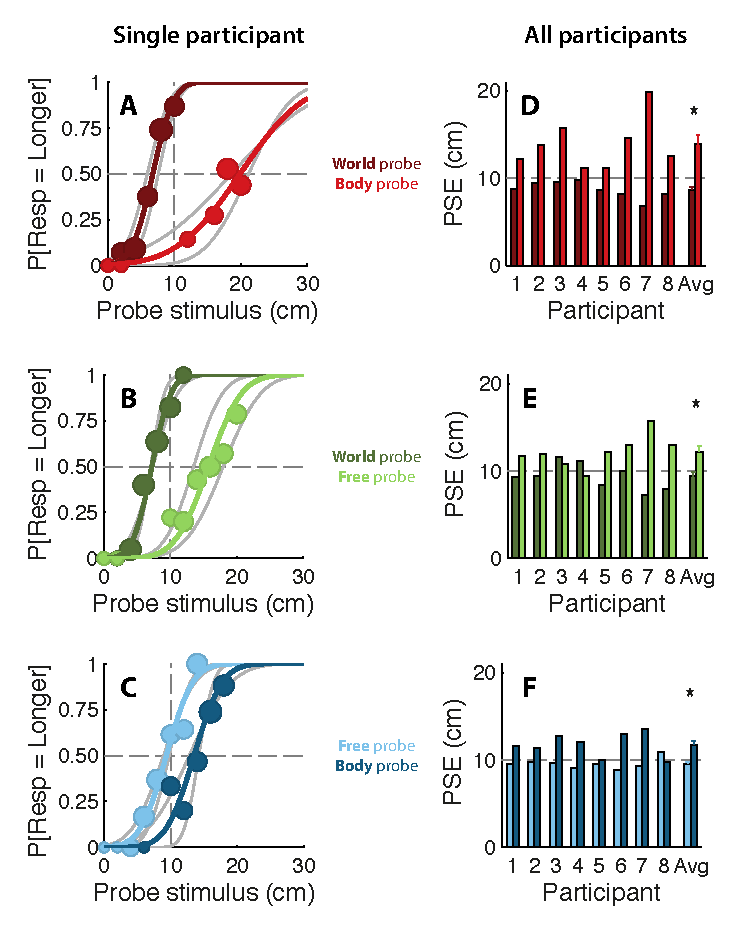
\includegraphics[width=1.0\textwidth]{src/paper3/figure2.pdf}

    \caption{Psychometric curves (colored lines) and associated binned data (circles) for one participant (top row). Circle size represents the number of trials within each 2 \si{\centi\metre} bin. Binning was only done in order to visualize this participant's responses and was not used otherwise. Gray lines show psychometric curves before collapsing across reference order. \panelref{A} Body-world comparison; body reference, dark red; world reference, light red. \panelref{B} World-free comparison; world reference, light green; free reference, dark green. \panelref{C}  Body-free comparison; body reference, dark blue; free reference, light blue. \newline
PSEs for all participants and the average {\textpm}SE (bottom row). \panelref{D} Body-world (dark red) and world-body (light red) conditions. \panelref{E} World-free (light green) and free-world (dark green) conditions. \panelref{F} Body-free (dark blue) and free-body (light blue) conditions. Because a t-test revealed a main effect of reference order, \ttest{47}{-5.2}{0.01}, we used the mean PSE across reference order (e.g. \figref{p3:fig3}, gray lines) instead of the PSE collapsing across reference order (e.g. \figref{p3:fig3}, colored lines); these values were not significantly different.}
    \label{p3:fig2}
\end{figure}

The performance of one participant is illustrated in the left column of \figref{p3:fig2}. Each row shows one main condition: body versus world fixation (top/red), world versus free fixation (middle/green), and body versus free fixation (bottom/blue). The lighter and darker colors in each panel indicate which fixation type was the reference movement (see Legend). The shift of the psychometric functions relative to the 10 \si{\centi\metre} reference (i.e. the PSE) quantifies the influence of fixation type. For example, the rightward shift of the light red curve in \figref{p3:fig2}A means that for a body fixation a longer translation (\about 19 \si{\centi\metre}) was required for that translation to be perceived equivalent to a 10\si{\centi\metre} reference translation with world fixation. On the other hand, the leftward shift of the dark red curve means that a shorter translation with world fixation (\about 7 \si{\centi\metre}) was required for that translation to be perceived equivalent to the 10 \si{\centi\metre} reference translation with body fixation. Together, these oppositely directed shifts demonstrate that translations with world fixation were perceived longer than equivalent translations with body fixation, regardless of which translation was the reference.  Similarly, the shifts in \figref{p3:fig2}B shows that world fixation translations were also perceived to be longer than free fixation movements and \figref{p3:fig2}C shows that free fixation translations were perceived to be longer than body fixation translations. Note that Figure 2 also shows an effects on slope, which will be further discussed in the paragraph \nameref{p3:sec:precision}.

Similar results were obtained for all subjects, as shown by the individual PSEs for all participants (right column of \figref{p3:fig2}). Statistical significance of the fixation-induced effects for each main condition (world versus body, \figref{p3:fig2}D; world versus free, \figref{p3:fig2}E; and free versus body, \figref{p3:fig2}F) was evaluated by comparing PSEs between the two reference conditions using a paired t-test. These PSEs were significantly different in all cases (world versus body, \ttest{7}{-4.09}{0.05}; world versus free, \ttest{7}{-2.48}{0.05}; free versus body, \ttest{7}{-3.38}{0.05}. As for the example subject, these results indicate that translations made with body fixation are perceived shorter than with world fixation, suggesting that self-motion perception is modulated by eye movements even in absence of full-field optic flow. The free fixation translations, which controlling for confounds of the small the fixation point, were perceived to be longer than body and shorter than world fixation translation intervals, which could be expected if their gain would be smaller than 1 but larger than 0.

\begin{figure}
    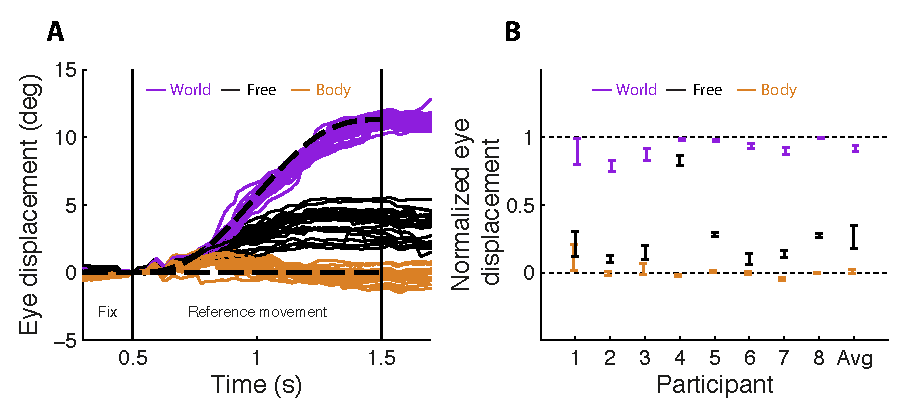
\includegraphics[width=1.0\textwidth]{src/paper3/figure3.pdf}

    \caption{\panelref{A} Actual (solid lines) and ideal (dashed lines) eye movement traces of one participant during world fixation (purple), body fixation (brown), and free fixation (black). All traces shown are for 10 \si{\centi\metre} reference movements. \panelref{B} Normalized eye position for each participant (\textpm95\% confidence interval) at the end of translation interval (error bars) for world fixation (purple), body fixation (brown) and free fixation (blue). In addition, the average {\textpm}SE across all participants is shown. Zero indicates that the eyes remained stationary relative to the body, and one indicates that eye position was perfectly world-fixed.}
    \label{p3:fig3}
\end{figure}

\subsection{Eye movement contributions to self-motion perception}

In order to relate psychophysical performance to eye movement behavior we recorded and analyzed eye movements during both intervals of every trial for all subjects. Exemplar eye traces for the 10 \si{\centi\metre} reference translation for the three fixation types are depicted in \figref{p3:fig3}A. Fixation behavior was quite accurate for both body fixations, where no eye movements were expected, and world fixation, where eye movement excursions of \siang{11} were expected, seemingly supported by  catch-up saccades. Under free fixation, the amount of eye movement was intermediate between body and world fixation and behavior was more variable. A similar pattern was observed in all participants, as illustrated by the normalized eye movement data (see \nameref{p3:sec:methods}, and \figref{p3:fig3}B).

\begin{figure}
    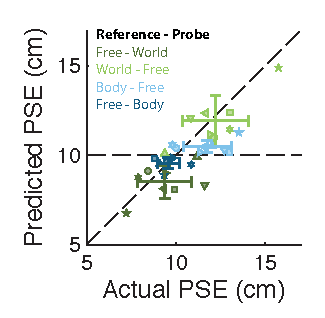
\includegraphics[width=0.5\textwidth]{src/paper3/figure4.pdf}

    \caption{Eye movement based prediction for the PSE plotted against the actual PSE.  A data point (symbol) is shown for each participant (symbol shape) and condition (symbol color) pair, following the same color scheme as in \figref{p3:fig2}. The identity line, corresponding to a perfect prediction, is shown in black.}
    \label{p3:fig4}
\end{figure}

\begin{table}
    \begin{tabular}{llll}
    Participant & Parameter ($\alpha$) \textpm SD \\
    \hline
    1 & 0.27 (\textpm 0.04) \\
    2 & 0.27 (\textpm 0.05) \\
    3 & 0.35 (\textpm 0.04) \\
    4 & 0.06 (\textpm 0.04) \\
    5 & 0.13 (\textpm 0.03) \\
    6 & 0.33 (\textpm 0.04) \\
    7 & 0.58 (\textpm 0.02) \\
    8 & 0.21 (\textpm 0.02) \\    
    \end{tabular}
    
    \caption{Estimated eye movement contribution (α) to the perception of self-motion (see Equation 5). Standard deviations are based on a bootstrap for each participant.}
    
    \label{p3:tab2}
\end{table}

To quantify the role of eye movements in self-motion, we tested a linear model in which perceived translation is a weighted average of a vestibular estimate (equal to the actual translation) and an oculomotor estimate (equal to the normalized eye movement times the actual translation; \eqnref{p3:eq2}). This model contains a single free parameter ($\alpha$), which corresponds to the relative weight given to the oculomotor estimate. We fitted this model to the two body versus world conditions and obtained the value of the oculomotor weight for every subject (\tabref{p3:tab2}). The average oculomotor weight is 0.25 \textpm0.12 (SD), indicating that the contribution of the eye movement signal to the self-motion estimate is about 25 percent. Note that participant 4, whose oculomotor weight is furthest from this mean ($\alpha = 0.06$), also shows a radically different eye movement gain during the free-fixation (see \figref{p3:fig3}B). We then used these oculomotor weights along with the normalized eye movement values to predict the PSEs in the remaining four conditions according to \eqnref{p3:eq5}. The predicted PSEs are plotted against the actually observed PSEs in \figref{p3:fig4}. The positive correlation ($\rho = 0.78$, $p < 0.01$) between observed and predicted PSEs suggests that eye movements are indeed used in self-motion perception, even in the absence of a fixation point (i.e. during free fixation). Furthermore, the fact that data points generally cluster near the unity line shows that our simple model does reasonably well in predicting perceptual performance across subjects and conditions based on oculomotor weight and normalized eye movement magnitude only. This holds true even for subject 7 whose oculomotor weight (\tabref{p3:tab2}) was approximately double the average, yet whose data points remain close to the unity line.

\begin{figure}
    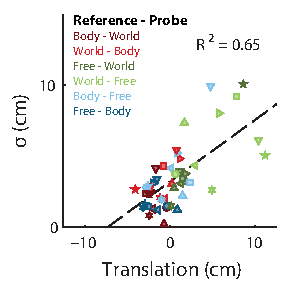
\includegraphics[width=0.5\textwidth]{src/paper3/figure5.pdf}

    \caption{Effect of difference movement amplitude between reference and probe interval (i.e. the bias) on response uncertainty ($\sigma$). A data point is shown for every participant and condition (symbol color) pair, following the same color scheme as in \figref{p3:fig2}. The dashed black line is the linear regression trend line.}
    
    \label{p3:fig5}
\end{figure}

\subsection{Precision depends on the PSE}
\label{p3:sec:precision}

The psychometric curves of the example participant in \figref{p3:fig2} show that precision ($\sigma^{-2}$ in \eqnref{p3:eq1}) decreases as the difference between translated distance in the reference and probe intervals (i.e. the bias) increases. To further investigate this effect, \figref{p3:fig5} shows a linear relation ($R^2 = 0.64$) between the bias and precision across all participants and conditions. This effect, which follows Weber’s perceptual law \cite{fechner1860} is consistent with the signal-dependence of (discrimination) precision that has been shown recently for vertical self-motion \cite{nesti2014}.


\section{Discussion}

We investigated the contribution of eye movements to the perception of passively-induced self-motion. Experiments were performed in the absence of full-field optic flow to eliminate the contribution of this visual motion signal. Perception of self-motion was compared across three fixation types: during free fixation the fixation target was extinguished before the movement, while during world and body fixation targets remained stable relative to the world and body, respectively. Our results show that self-motion is underestimated during body fixation (in which the eyes remain stationary) compared to world fixation (in which the eyes move to maintain fixation). To characterize the separate vestibular and eye movement contributions, we fitted a single parameter model to the perceptual responses for the body versus world comparison conditions and validated this model independently by predicting the effects of eye movements on self-motion perception during free fixation conditions. This model takes into account subject specific oculomotor weight and eye movement patterns. Based on these inputs it accurately predicts the responses in the free fixation conditions. This demonstrates that extra-retinal eye movement signals are used as a cue in the perception of self-motion, contributing significantly to the self-motion percept with a weight of approximately 25 percent, even in the absence of optic flow.

It is surprising that an influence of eye movements can be observed even for body- stationary fixations, during which the stationary eye movement signal is clearly in conflict with the non-zero vestibular signal. While this demonstrates the strength of the assumption that fixation targets are world-stationary, it raises the question how reliable this assumption is. Simultaneous recording of angular head and eye movements during natural behavior reveals that approximately 80 percent of eye movements can be classified as compensatory, i.e. eye movements directed opposite to head movement and therefore consistent with maintenance of world-fixed fixation \cite{einhauser2007}. Similarly, other studies have shown that world-stationary fixations are common for many every day activities, ranging from making a cup of tea \cite{hayhoe2014} to driving a car \cite{land1994}, to walking \cite{foulsham2011} and even reaching, where people tend to look at the source and destination of the object, but not at the hand \cite{flanagan2003}. Because world-stationary fixations are so common, the natural world statistics imply that self-motion and eye movements are highly correlated, thus making eye movements a fairly reliable cue for self-motion.

Even when fixation is not world-fixed, eye movement signals are combined with optic flow signals to yield realistic self-motion estimates (e.g. \cite{royden1992,vandenberg2000}). During world-fixed fixation, the eyes move to compensate for body translation, thereby reducing the optic flow component in the retinal signal. The self-motion estimate will therefore be driven predominantly by the eye movement signal. On the other hand, in the body-fixed condition, eye movements are minimal and optic flow maximal such that perceived self-motion will be driven predominantly by the optic flow signal itself. Because our experiment was performed in darkness, this optic flow signal was absent in the body-fixed condition which can explain why self-motion was underestimated.

During body and world fixation, eye movements are driven by retinal slip of the fixation target. However, in the free fixation condition, retinal slip is not available and resulting eye movements resemble the linear vestibulo-ocular reflex (LVOR), in that the gain relative to world fixation was ~0.4 (see Figure 3B; \cite{ramat2003}). This reflex is thought to be driven by a double integration of the vestibular signal, converting the head acceleration signal from the otoliths to eye position \cite{green2007,walker2010}. If eye movements during free fixation are in fact vestibularly driven, then combination of this eye movement signal with the vestibular signal itself seems redundant. However such combination could reflect a strategy to reduce noise. Both the direct (vestibular) and indirect (LVOR) signals depend on integration of the linear acceleration signal and may be corrupted by independent noise sources. Combining them in a statistically optimal fashion will decrease the noise level towards the noise level of the original source signal \cite{faisal2008,clemens2011,fetsch2013}. The consequence of this integration will be a reduced self-motion estimate when the gain of the LVOR is less than 1, as we observed in the free condition.
Alternative interpretations

In the above, we assumed that the eye movements themselves drive perception of self-motion. However, it is conceivable that a common correlate of eye movements, such as attention or visual motion influenced our results. In 1963, Guedry and Harris reported a substantial underestimation of displacement when their observers watched a small body-fixed target compared to displacements in the dark. However, they attributed their findings to an attentional shift from judgments of body displacement in the dark to judgments of target displacement in the fixation condition. Although our results are in line with their observations, our eye movement analysis as well as the relation to perceptual judgments suggest that eye movements modulate self-motion perception, possibly in addition to attentional factors \cite{kitazaki2003}.

Others have reported errors in the disambiguation of self and object-motion. Examples include the perceived motion of body-fixed visual targets during angular acceleration (the oculogyral illusion; \cite{carriot2011}), the apparent displacement of body-fixed stimuli during linear acceleration (the oculogravic illusion; \cite{graybiel1952}) and the apparent movement of world-stationary targets during self-motion in darkness \cite{dyde2008}. Similar disambiguation errors could cause the effects we observed. More specifically, if movement of the fixation point relative to the observer were always attributed to self-motion, then self-motion would be underestimated during body relative to world fixation, as we observed. However, such attribution errors cannot account for the effects in the free condition, because no fixation point was visible and no attribution was required. In the free condition, we demonstrate that eye movements by themselves, occurring in the absence of visual tracking and other external cues, influence the perception of self-motion.

\subsection{Implications for other studies}

Many previous self-motion studies have used a body-fixed fixation point to control for eye movement related effects. Our results suggest, however, that using a body-fixed fixation point causes underestimation of self-motion. For example, Li, Wei, and Angelaki \citeyear{li2005a} (2005) investigated spatial updating across lateral translation and found that saccades to updated targets undershot the actual target location. As self-motion perception drives this update, the effects of eye movements on self-motion perception should also influence the updating process. In other words, the observed undershoot could be due to the underestimation of self-motion caused by the body-fixed fixation point. Another example is a study on the perception of vertical object-motion during lateral translation \cite{dokka2013}. This study reports incomplete compensation for self-motion when judging the deviation from vertical motion of a moving object. This observation could also be due to underestimation of self-motion induced by the fixation of the body-fixed target. 

A moving fixation point is also known to influence self-motion perception, as in the Slalom Illusion \cite{freeman2000}; observers viewing expanding optic flow while fixating a target that oscillates from left to right perceive slaloming motion which is inconsistent with the purely forward motion specified by the expanding optic flow display. However, this observation is consistent with the idea that oculomotor signals are used in estimating self-motion. Additionally, it has been shown that eye movements affect postural sway \cite{glasauer2005}.  Participants performed smooth pursuit eye movements in complete darkness and displayed lateral sway consistent with the stabilization of posture using a self-motion estimate influenced by pursuit eye movements.

Studies conducted to characterize vestibular-only sensitivity are often performed in complete darkness or with closed eyes \cite{grabherr2008,macneilage2010b,macneilage2010a,roditi2012,valko2012,nesti2014}. However, the results of our free-fixation condition suggest that even under these circumstances, results could easily be influenced by vestibularly driven eye movements. Overall, we suggest that any study concerned with self-motion processing must consider the possible influence of eye movements.

\subsection{Possible neural substrate}

This leaves us with the question of where in the brain these effects originate. The locus of our effect is likely to carry both eye movement and vestibular signals. Prime candidate areas known to carry both vestibular and eye movement signals are the vestibular nuclei \cite{henn1975,daunton1979} and the cerebellum \cite{waespe1981}. On the other hand, eye movements could influence self-motion perception indirectly via optic flow processing. In particular, cortical areas that carry both vestibular and optic flow signals (which can be modulated by eye movements) include the ventral intraparietal area (VIP; \cite{bremmer2002,chen2011}), and the dorsal medial superior temporal area (MSTd; \cite{gu2008}). Future work should reveal how such brain areas, directly or indirectly, merge both vestibular and oculomotor signals into a coherent percept of self-motion.



\bibliography{refs}{}

\titleformat{\chapter}
{\normalfont\Large\bfseries}{\thechapter}{0.2em}{}
\titlespacing*{\chapter}{0pt}{-30pt}{10pt}

\end{document}

\chapter{Paper 4}
\chaptermark{}

\newpage
...
\chapter{Summary and discussion}

Navigating through the environment evokes complex changes of visual, auditory, vestibular, tactile and
motor inputs to the brain. Yet, despite this motion, we perceive the world as a stable reality, maintain an integrated sense of where we are, how we are oriented, and are able to track and act rather effortlessly upon surrounding objects.  How the ability comes about it one of the key questions in neuroscience and also studied in this research project. The objective was to build computational models and perform thorough psychometric testing in order to examine the physical and biological contrast that are placed on the interaction between the vestibular and other sensory systems for spatial orientation and self-motion perception. This resulted in the following contributions to the field:

\begin{enumerate}
\item Statistical optimality can account for the way body somatosensory, neck proprioceptive and vestibular signals are integrated in spatial orientation perception. While these sensors cannot be examined in isolation, by using optimality as a starting point, their noise properties can be determined and linked to clinical deficits that are seen in particular patient groups.
\item Oculomotor signals influence self-motion perception, even in the absence of optic flow or other visual stimulation, and even when in conflict with vestibular information. 
\item This oculomotor signals should be regarded as rudimentary cue to self-motion perception; it is not veridically scaled by fixation distance in the perception of body translation. 
\item Self-motion signals interact with the dynamic perception of external world.  Errors that arise in this process suggest the use of a gaze-centered reference frames in the underlying computations. 
\end{enumerate}

In the following sections, we will provide a detailed summary of each result. 

\section{Multisensory processing in spatial orientation}
Many studies have shown that the brain tends to combine noisy sensory signals in a statistically optimal way. This is normally done by showing that the noise levels of each separate modality can predict performance in combined conditions. In spatial orientation it is difficult to measure sensory signals in isolation as multisensory integration always takes place. In Chapter 2 we therefore used a statistically optimal integration model as a starting point, and attempted to account for the perceptual differences found when probing head-in-space versus body-in-space orientation. Using a psychometric approach, we tested both the perception of body tilt (subjective body tilt; SBT) as well as the perception of visual vertical (subjective visual vertical; SVV) in seven participants. Our model was able to explain the results from both tests. Because one of sensory modalities used, the noise in the neck proprioceptors, can be measured in relative isolation, we used it to independently confirm the predicted head-on-body noise found by the model. We further validated our model by showing that predictions made by our model are consistent with previously published deficits in vestibular and somatosensory patients. We conclude that Bayesian computations can account for the typical differences in spatial orientation judgments associated with different task requirements.

\section{Eye movements influence self-motion perception}
Eye movement typically accompany self-motion in order to minimize retinal slip and maximize dynamic visual acuity. In Chapter 3 we investigate whether these eye movements also have a reversed role, serving as a cue for self-motion perception. To address this question, we asked participants to compare perceived translation distance in two successive, passive, lateral whole-body translations. Eye movements during these translations were either world-stationary or body-stationary. Results show that translations were perceived shorter with body-fixed gaze compared to world-fixed gaze, indicating that eye movements indeed influence self-motion perception. Using a linear model, we estimated the relative contribution of the vestibular versus the eye movement signal, and found that eye movement signals contribute approximately 25 percent of the perceived motion. We independently validated the model by successfully predicting the effects of eye movements on self-motion perception during trails in which the eye movements were unconstrained. This further shows that eye movement signals influence self-motion perception, even in the absence of visual stimulation, and even when oculomotor and vestibular estimates are in conflict, e.g. during body-fixed gaze. We hypothesize that adverse consequences of this seemingly inflexible arrangement are minimal under natural conditions because eye movements and self-motion are highly correlated, and because eye movements are most often accompanied by veridical optic flow cues to self-motion.

\section{Partial compensation for fixation depth in self-motion perception}
The amplitude of these eye movements depend on the depth of fixation, when fixating  faraway they are smaller than when fixating nearby in the world. If these eye movements are used to augment self-motion perception, the effect of fixation depth has to be taken into account in order for self-motion perception to be veridical. In Chapter 4 we investigate whether the brain indeed compensates and takes fixation depth into account. Participants had to judge self-motion during different eye movement conditions in the absence of full-field optic flow. In a 2-AFC task, similar to the one used in Chapter 3, participants indicated whether the second of two successive passive lateral whole-body translations was longer or shorter than the first. During each translation, participants fixated either a nearby or far away target, which was either body- or world-stationary. Results show that the perceived translations were shorter for nearby world-fixed gaze compared to far away world-fixed gaze, indicating that eye movements are not properly scaled in self-motion perception. Together with the observation that self-motion perception is not affected by the depth of a body stationary fixation target, we conclude that eye movements are merely a rudimentary cue to self-motion, with a compensation for fixation depth that is partial at best.

\section{Gaze-dependent effects in spatial updating}
The brain uses these self-motion signals to update ego-centric spatial representations of the environment. In Chapter 5 we investigate how, and to which extent, the brain integrates these various self-motion signals for the spatial update. Participants were oscillated sideways while keeping gaze fixed on a stationary target. When the motion direction changed, a reference target was shown either in front or behind the fixation point. Half a cycle later, at the next reversal, we tested updating of this reference location by asking participants to judge whether a briefly flashed probe was shown to the left or right of the memorized target. Results show that both the direction and magnitude of the bias in spatial updating depends on the location of the object being updated with respect to gaze, implying that a gaze-centered reference frame is involved. We further show that these biases can be caused by an underestimated of translation amplitude, a bias of visually perceived objects towards the fovea, or by a combination of both.

\section{Concluding remarks}

To integrate multiple redundant sensory signals into a single percept, the brain commonly employs a process called Bayesian integration (see Chapter 1). In this process both sensory signals as well as prior information about the environment are combined by weighting them by their relative precision. Inversely, by assuming Bayes’ optimal integration it is, for some systems, possbile to estimate the precision of sensory signals. In Chapter 2 we have demonstrated this concept for spatial orientation perception.

In Chapter 3 and 4 we have introduced eye movements as a novel cue to self-motion. Whether these  eye movements are integrated with out self-motion cues in a statiscially optimal fashion remains an open question, as our models did not take precision into account. While we hypothesize that this is indeed  the case, the weight of the oculomotor signal might not be easily determined.

Fixation targets can be world-stationary, body-stationary or somewhere in-between. Only when a fixation target is world-stationary should the eye movement signal be used for self-motion perception, otherwise it is uninformative. From a probablisitic perspective, one would weight the self-motion estimate given a world-stationary target (x=ed) and the estimate given a body-stationary target (x=0) based on the relative probability of the fixation target beging world- or body-stationary respectively. In darkness only prior knowledge can be used, and we hypothesize that the prior probability of fixating a world-stationary target is high. This in turn causes the eye movement signal to have a significant weight and thus contribution to the oculomotor based self-motion estimate. The reliability of the oculomotor signal can be weighted in a similar way, taking the probability of  world- versus body-stationary fixations into account.

In Chapter 5 we show that eye movements are taken into account when updating the remebered location of previously seen targets. If the same signal used for self-motion perception influences spatial updating, then the type of fixation (world- versus body-stationary) should have an effect on spatial updating as well. Furthermore any increase in noise due to the  updating process should be proportional to the differences in noise observed in the oculomotor-based self-motion estimates. 

We have performed a pilot experiment where participants had to reach towards remembered targets after intervening translation. Preliminary results suggest that reaching errors are large when fixating a  body-stationary target during translation, while no such errors exist while fixating world-stationary targets \cite{clemens2010}. Suggesting that the eye-movement based self-motion cues are indeed used in spatial updating.
 


%%%%%%%%%%%%%%
% Back matter

\backmatter

\bibliography{refs}{}

\titleformat{\chapter}
{\normalfont\Large\bfseries}{\thechapter}{0.2em}{}
\titlespacing*{\chapter}{0pt}{-30pt}{10pt}

\selectlanguage{dutch}
\clearpage
\pagestyle{empty}

\chapter*{Nederlandse samenvatting}
\phantomsection
\addcontentsline{toc}{chapter}{Nederlandse samenvatting}

Navigeren door de omgeving oproept complexe veranderingen van visuele, auditieve, vestibulaire, tactiele en
motor inputs naar de hersenen. Toch, ondanks deze beweging veroorzaakte veranderingen van de input, we de wereld waarnemen als een stabiele werkelijkheid, maar ook een geïntegreerde gevoel van waar we zijn, hoe we zijn gericht, en in staat zijn op te sporen en te handelen in plaats moeiteloos op omliggende objecten. Hoe dit vermogen komt is ook het onderwerp van dit proefschrift. Het doel van het onderzoek beschreven in dit proefschrift was om computationele modellen op te bouwen en uit te voeren grondige psychometrische tests om de fysische en biologische beperkingen te ontrafelen op de interactie tussen het evenwichtsorgaan en andere sensorische systemen voor ruimtelijke oriëntatie en zelf-waarneming van beweging. Dit resulteerde in de volgende bijdragen aan het veld:

\ Begin {description}
\ Item [\ hoofdstuk {p1}] Statistische optimaliteit kan goed zijn voor de manier waarop het lichaam somatosensorische, zijn nek proprioceptieve en vestibulaire signalen geïntegreerd in ruimtelijke oriëntatie waarneming. Hoewel deze sensoren niet afzonderlijk kan worden onderzocht door optimaliteit als uitgangspunt geluidsemissie eigenschappen kunnen worden bepaald en gekoppeld aan klinische afwijkingen die worden gezien name patiëntengroepen.
\ Item [\ hoofdstuk {p3}] oogmotorische signalen beïnvloeden eigen waarneming van beweging, zelfs in afwezigheid van optic flow of andere visuele stimulatie, en zelfs in strijd met vestibulaire informatie.
\ Item [\ hoofdstuk {p4}] Dit oculomotorische signalen moet zo rudimentair cue om zelf-waarneming van beweging worden beschouwd; Het is niet veridically geschaald fixatie afstand in de perceptie van lichaam vertaling.
\ Item [\ hoofdstuk {p2}] Self-motion signalen interactie met de dynamische perceptie van de buitenwereld. Fouten die zich voordoen bij deze werkwijze suggereren het gebruik van een blik gecentreerd referentieframes in de onderliggende berekeningen.
\ End {description}

In de volgende paragrafen zullen we een gedetailleerd overzicht van elk resultaat te bieden.

\ Section {Multisensorische verwerking in ruimtelijke oriëntatie}
Vele studies hebben aangetoond dat de hersenen combineert luidruchtige sensorische signalen in een statistisch optimale wijze. Dit gebeurt normaal door te laten zien dat het geluidsniveau van elke afzonderlijke modaliteit prestaties in combinatie kunnen voorspellen. In ruimtelijke oriëntatie is het moeilijk om zintuiglijke signalen afzonderlijk te meten als men niet kan uitschakelen het vestibulair gevoel bij het meten van somatosensorische bijdragen. In \ hoofdstuk {p1} daarom gebruikten we een statistisch optimale integratie-model als uitgangspunt, en geprobeerd om rekening te houden met de perceptuele verschillen gevonden wanneer indringende kop-in-ruimte versus body-in-ruimte oriëntatie. Met een psychometrische benadering, testten we zowel de perceptie van lichaam tilt (persoonlijke gesl; SBT) en de waarneming van visuele verticale (subjectieve visuele verticaal, SVV) in zeven deelnemers. Omdat zowel de SVV en SBT maken gebruik van dezelfde zintuiglijke signalen, waren we in staat om een ​​7-parameter probabilistische model past bij de respons gegevens. Een van de geschatte parameters vertegenwoordigde het lawaai van de nek proprioceptoren. Dit liet ons toe om onafhankelijk te bevestigen dat de verkregen waarden voor de hals geluid overeen met die die werden gemeten in isolement. We verder gevalideerd ons model door te laten zien dat voorspellingen van ons model zijn in overeenstemming met eerder gepubliceerde tekorten in vestibulair en somatosensorische patiënten. We concluderen dat de Bayesiaanse berekeningen kan goed zijn voor de typische verschillen in ruimtelijke oriëntatie oordelen in verband met verschillende vereisten van de taak. In een vervolg op dit werk, werd deze aanpak onlangs toegepast op een patiëntenpopulatie met complete vestibulair verlies \ cite {alberts2015}. Prestaties in die patiënten vergelijkbaar met die van de controles, wat suggereert dat de sensorische gewicht was verschoven van de vestibulaire de somatische sensors.

\ Section {Oogbewegingen beïnvloeden zelf-waarneming van beweging}
Eye movement begeleiden meestal zelf-beweging om het netvlies slip minimaliseren en maximaliseren dynamische gezichtsscherpte. In \ hoofdstuk {p3} hebben we onderzocht of deze oogbewegingen hebben ook een omgekeerde rol, door te dienen als een cue voor zelf-waarneming van beweging. Om deze vraag te beantwoorden, vroegen we de deelnemers om gepercipieerde vertaling afstanden vergelijken van twee opeenvolgende, passieve, laterale hele lichaam vertalingen. Oogbewegingen tijdens deze vertalingen waren ofwel wereld-stationaire of body-stationaire. Resultaten laten zien dat de vertalingen korter werden waargenomen met body-fixed blik in vergelijking met-wereld vaste blik, wat aangeeft dat de oogbewegingen inderdaad beïnvloeden self-waarneming van beweging. Met behulp van een lineair model, schatten we de relatieve bijdrage van de vestibulaire versus de oogbeweging gebaseerd verplaatsingssignaal: de oogbeweging gebaseerd verplaatsingssignaal draagt ​​ongeveer 25 procent tot de waargenomen beweging. We onafhankelijk gevalideerd het model door het succes voorspellen van de effecten van oogbewegingen op zelf-waarneming van beweging tijdens de studies waarin de oogbewegingen waren ongedwongen. Dit toont verder dat oogbeweging signalen beïnvloeden eigen waarneming van beweging, zelfs zonder visuele stimulatie, en zelfs wanneer oculomotorische en vestibulaire schattingen in conflict, zoals tijdens-orgaan vastgestelde blik. We veronderstellen dat de nadelige gevolgen van deze schijnbaar starre opstelling minimaal zijn onder natuurlijke omstandigheden, omdat de oogbewegingen en zelf-beweging sterk gecorreleerd zijn, en omdat de oogbewegingen worden meestal begeleid door veridical optic flow aanwijzingen om zelf-beweging.

\ Section {gedeeltelijke compensatie voor fixatie diepte in zelf-waarneming van beweging}
Als oogbewegingen worden gebruikt bij de schatting van zelf-motion magnitude dient de hersenen ook de bijbehorende fixatie diepte slaan bij een veridical vertaling schatting. De reden is dat de amplitude van deze oogbewegingen, voor dezelfde fysieke vertaling, afhankelijk van de diepte van fixatie: als verre fixeren ze kleiner dan wanneer de omgeving fixeren in de wereld. In \ hoofdstuk {p4} hebben we onderzocht of de hersenen neemt inderdaad fixatie diepte te houden bij het gebruik van oogbewegingen om zelf-waarneming van beweging te vergroten. De deelnemers moesten zelf-motion tijdens verschillende omstandigheden oogbewegingen in de afwezigheid van full-field optic flow oordelen. In een 2-AFC taak, vergelijkbaar met die gebruikt in \ hoofdstuk {p3} deelnemers aangegeven of de tweede van twee opeenvolgende passieve zijdelingse gehele lichaam vertalingen langer of korter dan de eerste was. Tijdens elke vertaling, deelnemers gefixeerd ofwel een in de buurt of ver weg doelgroep, die ofwel lichaams- of world-stationaire was. Resultaten laten zien dat de waargenomen vertalingen waren korter voor nabijgelegen-wereld vaste blik in vergelijking met verre-wereld vaste blik, wat aangeeft dat de oogbewegingen niet goed geschaald in zelf-waarneming van beweging. Samen met de observatie dat zelf-waarneming van beweging niet wordt beïnvloed door de diepte van een lichaam stationaire fixatie doelgroep, kunnen we concluderen dat de oogbewegingen zijn slechts een rudimentaire cue om zelf-beweging, met een compensatie voor fixatie diepte die gedeeltelijke op zijn best.

\ Section {Gaze-afhankelijke effecten in ruimtelijke updating}
De hersenen moet ook zelf-beweging signalen naar ego-centrische ruimtelijke voorstellingen van het milieu te werken. In \ hoofdstuk {p2} onderzoeken we hoe, en in welke mate, de hersenen integreert de verschillende self-motion signalen voor de ruimtelijke-update. Deelnemers werden heen en weer geslingerd zijwaarts terwijl blik gericht op een stationaire doelwit. Wanneer de beweging richting veranderde, werd een verwijzing doel, hetzij voor of achter de fixatie punt getoond. Half een cyclus later, bij de volgende omkering, testten we bijwerking van de verwijzingen locatie door te vragen de deelnemers om te beoordelen of een kort flitste sonde werd getoond aan de linker- of rechterkant van de opgeslagen doel. De resultaten tonen aan dat zowel de richting en grootte van de bias in ruimtelijke bijwerking afhankelijk van de locatie van het object wordt geactualiseerd ten opzichte blik, hetgeen impliceert dat een blik centered referentiekader betrokken. We tonen verder aan dat deze vertekeningen kunnen worden veroorzaakt door een onderschat vertaling amplitude, een voorspanning van visueel waargenomen objecten naar de fovea, of door een combinatie van beide.

\ Section {Slotopmerkingen}

Alle experimentele hoofdstukken in dit proefschrift verslag over ruimtelijke beleving onderwerpen '. In \ hoofdstuk {p1} gebruiken we een optimale statistische integratiemodel van alle bijdragen sensorische systemen om zowel de bias en de precisie van deze waarnemingen te verklaren. In deze modellen de bijdragen van de zintuigen worden gewogen op basis van hun onzekerheid. In de hoofdstukken over laterale verplaatsing perceptie (\ hoofdstuk {p3, p4}) gebruiken we ook de wegingen van het evenwichtsorgaan en oog-beweging gebaseerde ramingen van de verplaatsing. Echter, deze weegt slechts op basis van de waargenomen biases in zelf-waarneming van beweging. Idealiter zou men dezelfde aanpak als in \ hoofdstuk {p1} te modelleren en analyseren van deze zelf-waarneming van beweging gegevens. We hebben eerste pogingen om een ​​dergelijke model gemaakt, maar verschijnen er tenminste twee belangrijke uitdagingen. Ten eerste, de geometrie van de zelf-waarneming van beweging experimenten maakt dat de eenvoudige Gauss uitkeringen van de ruimtelijke oriëntatie model te worden minder goed gedefinieerd, een scheve verdeling en we zouden moeten gebruiken roetfilter modellen om onze simulaties uit te voeren. Tweede, die modellen bevatten veel vrije parameters voor de zintuiglijke modaliteiten en priors. Met de huidige reeks experimenten we niet genoeg data om deze parameter te passen op een consistente manier te hebben. Toekomstig onderzoek moet worden gedaan om een ​​complete optimale rekening integratie van zelf-waarneming van beweging af te leiden.

In \ hoofdstuk {p2} laten we zien dat oogbewegingen uitgelokt door het fixeren van een wereld-stationaire doelwit worden in aanmerking genomen bij het updaten van de herinnerde locatie van eerder gezien doelen. Als de onderliggende signalen gebruikt voor zelf-waarneming van beweging zoals gevonden in \ hoofdstuk {p3, p4} worden ook gebruikt voor ruimtelijke bijwerken, het soort fixatie (wereld- versus body-stationaire) een effect op de waargenomen biases in ruimtelijke actualisering zou moeten hebben ook. Inderdaad, de resultaten van een proefproject in het vroege stadium van dit proefschrift suggereren dat Type fixatie beïnvloedt ruimtelijke bijwerken prestaties onder vertaling \ cite {clemens2010}. Deelnemers moesten bereiken richting herinnerde doelen na een tussenliggende vertaling. Voorlopige resultaten wijzen erop dat het bereiken van fouten zijn groot wanneer het fixeren van een body-stationaire doelwit tijdens de vertaling, terwijl er geen dergelijke fouten bestaan, terwijl het fixeren van wereldklasse stilstaande doelen \ cite {clemens2010}, wat suggereert dat inderdaad de eye-beweging gebaseerde self-motion signalen worden ook gebruikt in de ruimtelijke bijwerken.

Tot slot hoop ik nieuwe ontwikkelingen te hebben gemaakt in het begrip van de mechanismen voor ruimtelijke oriëntatie en zelf-waarneming van beweging. Natuurlijk, er zijn veel resterende vragen voor verdere studie. Deze onderzoeken moeten in de eerste plaats richten op de computationele en theoretische mechanismen, en hoe ze worden uitgevoerd door de neurale circuits. Deze studies moeten niet alleen het adres van de computationele en theoretische mechanismen, maar ook op de neurale implementatie en routes die kunnen worden gevonden in de hersenen.


\selectlanguage{british}
\clearpage
%\pagestyle{empty}

\chapter*{Curriculum vitae}
\phantomsection
\addcontentsline{toc}{chapter}{Curriculum vitae}

Ivar Clemens was born in 1984 in Boxtel, the Netherlands. After obtaining a degree in Industrial Automation at the Koning Willem 1 College in 's-Hertogenbosch, he started a master's degree in Biology at the Radboud University in Nijmegen, the Netherlands. In 2008 Ivar did his first research internship on the \emph{integration of pre- and post-vergence target distance cues} with Pieter Medendorp at the Nijmegen Institute for Cognition and Information (NICI, later renamed to the Donders Centre for Cognition). Ivar then switched to the Donders Centre for Cognitive Neuro-imaging (DCCN) for his second research internship. This time he worked with  Ole Jensen and Saskia Haegens on \emph{homeostatic plasticity in the somatosensory cortex}. He obtained his master's degree in 2009 and started his PhD research under the supervision of Pieter Medendorp and Luc Selen at the Donders Centre for Cognition. During his PhD he worked on the integration of sensory signals in spatial orientation and self-motion perception. In January 2015 he joined the group dynamics lab at the Champalimaud Centre for the Unknown in Lisbon, Portugal.

\clearpage
\pagestyle{empty}

\chapter*{List of publications}
\phantomsection
\addcontentsline{toc}{chapter}{List of publications}

About me
\clearpage
\pagestyle{empty}

\chapter*{Acknowledgments}
\phantomsection
\addcontentsline{toc}{chapter}{Acknowledgments}

First of all, I would like to extend my thanks to \textbf{my supervisors}, Pieter and Luc, who have been of crucial importance in designing, running, and writing up the experiments in this thesis as well as to my development as a researcher in general. Thanks to \textbf{my fiancee} Daphne and \textbf{my parents}, Marja en Wim, for their unconditional support and confidence in me while I was writing this thesis. p

Second, I would like to thank \textbf{my family} Thaja, Annika, Sjors, Marcel, and Billy, Lancy, Percy, Stephanie, and Tyra, and \textbf{my friends in Boxtel \footnote{Including Lennisheuvel and Vught}} Kees, Paul, Bram, Joukje, Marieke, and Lieke.


This thesis would not have been possible without the help of 
my \textbf{collaborators} Mathieu, Paul MacNeilage, and Gerine,
the awesome people of the
\textbf{technical support group} Chi, Gerard, Mark, Norbert, Pascal, Twan, and Wilbert,
as well as the support staff
\textbf{support team} Jolanda, Maaike, Saskia, and Yvonne.
I would also like to thank the members of the 
\textbf{sensorimotor lab} Adjmal, Anouk, Antonella, Arjen, Bart, Femke, Frank, Jeroen, Joost, Julian, Jurrian, Liliana, Luc, Maaike, Mathieu, Pieter, Romy, Sara, Stan, Tineke, and Verena 
as well as our 
\textbf{trainees} Alexanra, Anna, Charlotte, Jeroen, Koen, Michael, Nynke.
Many tanks to the other people in \textbf{room B1.29}, Jurrian, Zhong Lu, and Romy, you were all great people.


During my PhD I've started to explore the world, my trips wouldn't have been as enjoyable without 
\textbf{ECVP; Alghero and Bremen} Anouk, Bronagh, Chayada, Richard, Simon-Jan, and Xuyan,
\textbf{K\"oln} Verena, Mathias, Sybrine, Marlene, and Lisa,
\textbf{Les Sybelles} Anke Marit, Lisa, Rene, Roemer, Ruud, Sasha, Sybrine, Tim, and Tjerk.
\textbf{London} Ricarda,
\textbf{Oxford} De Stagekamer; Emily, Frauke, Heleen, Katharina, Lisa, Miriam, Roemer, Susanne, and Vincent
\textbf{S\~ao Paulo} Vit\'oria and Kris,
\textbf{T\"ubbingen} Sybrine.
I would like to thank Frank and Verena in particular for the awesome trip to the \textbf{United States} that started it all.


% Johanna, Alessandra


Over the years I have participated in many sporting events and practice sessions, thanks to all those who joined me in 
\textbf{basketball} Ashley, Claudia, Flora, Jonathan, Michaelis, and Svetlana,
\textbf{climbing} Claire,
\textbf{dancing} Lies,
\textbf{running} Eelco, Corina, Stan, Sasha, Anke Marit, Tom, Jeanette, Alina, Verena Ly, Sybrine, Tim, Ruud, Rene, Tom, and Haiteng,
\textbf{squash} Gabriela,
\textbf{triathlon} Jessica and Norbert, 
\textbf{volleyball} Arjen, Christian, Egbert, Florian, Loes, Maaike, Mark, Marlene, Marvin, Pascal de W., Pascal B., Kors, Roemer, Ruud, Sanne, Sara, Sarah, Sasha, Sebo, and Sybrine, 
and 
\textbf{walking} Anke-Marit, Alina, Erik, Johanna, Sebastiaan, Laurence, Mirjam, Desiree, and Bart.

Finally, I would like to thank everyone who did not fit in any of the above categories.

\clearpage
\pagestyle{empty}

\chapter*{Donders Graduate School for Cognitive Neuroscience Series}
\phantomsection
\addcontentsline{toc}{chapter}{Donders Series}%

%\noindent \begrip{}
\npar\npar
\footnotesize
\noindent 1.	Van Aalderen-Smeets, S.I. (2007). \emph{Neural dynamics of visual selection.} Maastricht University, Maastricht, the Netherlands.\npar \noindent 2.	Schoffelen, J.M. (2007). \emph{Neuronal communication through coherence in the human motor system.} Radboud University Nijmegen, Nijmegen, the Netherlands.\npar \noindent 3.	De Lange, F.P. (2008). \emph{Neural mechanisms of motor imagery.} Radboud University Nijmegen, Nijmegen, the Netherlands.\npar \noindent 4.	Grol, M.J. (2008). \emph{Parieto-frontal circuitry in visuomotor control.} Utrecht University, Utrecht, the Netherlands.\npar \noindent 5.	Bauer, M. (2008). \emph{Functional roles of rhythmic neuronal activity in the human visual and somatosensory system.} Radboud University Nijmegen, Nijmegen, the Netherlands.\npar \noindent 6.	Mazaheri, A. (2008). \emph{The influence of ongoing oscillatory brain activity on evoked responses and behaviour.} Radboud University Nijmegen, Nijmegen, the Netherlands.\npar \noindent 7.	Hooijmans, C.R. (2008). \emph{Impact of nutritional lipids and vascular factors in Alzheimer's disease.} Radboud University Nijmegen, Nijmegen, the Netherlands.\npar \noindent 8.	Gaszner, B. (2008). \emph{Plastic responses to stress by the rodent urocortinergic Edinger-Westphal nucleus.} Radboud University Nijmegen, Nijmegen, the Netherlands.\npar \noindent 9.	Willems, R.M. (2009). \emph{Neural reflections of meaning in gesture, language and action.} Radboud University Nijmegen, Nijmegen, the Netherlands.\npar \noindent 10.	Van Pelt, S. (2009). \emph{Dynamic neural representations of human visuomotor space.} Radboud University Nijmegen, Nijmegen, the Netherlands.\npar \noindent 11.	Lommertzen, J. (2009). \emph{Visuomotor coupling at different levels of complexity.} Radboud University Nijmegen, Nijmegen, the Netherlands.\npar \noindent 12.	Poljac, E. (2009). \emph{Dynamics of cognitive control in task switching: Looking beyond the switch cost.} Radboud University Nijmegen, Nijmegen, the Netherlands.\npar \noindent 13.	Poser, B.A. (2009). \emph{Techniques for BOLD and blood volume weighted fMRI.} Radboud University Nijmegen, Nijmegen, the Netherlands.\npar \noindent 14.	Baggio, G. (2009). \emph{Semantics and the electrophysiology of meaning. Tense, aspect, event structure.} Radboud University Nijmegen, Nijmegen, the Netherlands.\npar \noindent 15.	Van Wingen, G.A. (2009). \emph{Biological determinants of amygdala functioning.} Radboud University Nijmegen Medical Centre, Nijmegen, the Netherlands.\npar \noindent 16.	Bakker, M. (2009). \emph{Supraspinal control of walking: Lessons from motor imagery.} Radboud University Nijmegen Medical Centre, Nijmegen, the Netherlands.\npar \noindent 17.	Aarts, E. (2009). \emph{Resisting temptation: The role of the anterior cingulate cortex in adjusting cognitive control.} Radboud University Nijmegen, Nijmegen, the Netherlands.\npar \noindent 18.	Prinz, S. (2009). \emph{Waterbath stunning of chickens – Effects of electrical parameters on the electroencephalogram and physical reflexes of broilers.} Radboud University Nijmegen, Nijmegen, the Netherlands.\npar \noindent 19.	Knippenberg, J.M.J. (2009). \emph{The N150 of the Auditory Evoked Potential from the rat amygdala: In search for its functional significance.} Radboud University Nijmegen, Nijmegen, the Netherlands. \npar \noindent 
20.	Dumont, G.J.H. (2009). \emph{Cognitive and physiological effects of 3,4-methylenedioxymethamphetamine (MDMA or 'ecstasy') in combination with alcohol or cannabis in humans.} Radboud University Nijmegen, Nijmegen, the Netherlands. \npar \noindent 21.	Pijnacker, J. (2010). \emph{Defeasible inference in autism: A behavioral and electrophysiogical approach.} Radboud University Nijmegen, Nijmegen, the Netherlands.\npar \noindent 22.	De Vrijer, M. (2010). \emph{Multisensory integration in spatial orientation.} Radboud University Nijmegen, Nijmegen, the Netherlands.\npar \noindent 23.	Vergeer, M. (2010). \emph{Perceptual visibility and appearance: Effects of color and form.} Radboud University Nijmegen, Nijmegen, the Netherlands.\npar \noindent 24.	Levy, J. (2010). \emph{In cerebro unveiling unconscious mechanisms during reading.} Radboud University Nijmegen, Nijmegen, the Netherlands.\npar \noindent 25.	Treder, M. S. (2010). \emph{Symmetry in (inter)action.} Radboud University Nijmegen, Nijmegen, the Netherlands.\npar \noindent 26.	Horlings C.G.C. (2010). \emph{A weak balance: Balance and falls in patients with neuromuscular disorders.} Radboud University Nijmegen, Nijmegen, the Netherlands.\npar \noindent 27.	Snaphaan, L.J.A.E. (2010). \emph{Epidemiology of post-stroke behavioural consequences.} Radboud University Nijmegen Medical Centre, Nijmegen, the Netherlands.  \npar \noindent 
28.	Dado-Van Beek, H.E.A. (2010). \emph{The regulation of cerebral perfusion in patients with Alzheimer's disease.} Radboud University Nijmegen Medical Centre, Nijmegen, the Netherlands.  \npar \noindent 29.	Derks, N.M. (2010). \emph{The role of the non-preganglionic Edinger-Westphal nucleus in sex-dependent stress adaptation in rodents.} Radboud University Nijmegen, Nijmegen, the Netherlands.\npar \noindent 30.	Wyczesany, M. (2010). \emph{Covariation of mood and brain activity. Integration of subjective self-report data with quantitative EEG measures.} Radboud University Nijmegen, Nijmegen, the Netherlands.\npar \noindent 31.	Beurze S.M. (2010). \emph{Cortical mechanisms for reach planning.} Radboud University Nijmegen, Nijmegen, the Netherlands.\npar \noindent 32.	Van Dijk, J.P. (2010). \emph{On the Number of Motor Units.} Radboud University Nijmegen, Nijmegen, the Netherlands.\npar \noindent 33.	Lapatki, B.G. (2010). \emph{The Facial Musculature - Characterization at a Motor Unit Level.} Radboud University Nijmegen, Nijmegen, the Netherlands.\npar \noindent 34.	Kok, P. (2010). \emph{Word order and verb inflection in agrammatic sentence production.} Radboud University Nijmegen, Nijmegen, the Netherlands.\npar \noindent 35.	van Elk, M. (2010). \emph{Action semantics: Functional and neural dynamics.} Radboud University Nijmegen, Nijmegen, the Netherlands.\npar \noindent 36.	Majdandzic, J. (2010). \emph{Cerebral mechanisms of processing action goals in self and others.} Radboud University Nijmegen, Nijmegen, the Netherlands.  \npar \noindent 37.	Snijders, T.M. (2010). \emph{More than words - Neural and genetic dynamics of syntactic unification.} Radboud University Nijmegen, Nijmegen, the Netherlands.\npar \noindent 38.	Grootens, K.P. (2010). \emph{Cognitive dysfunction and effects of antipsychotics in schizophrenia and borderline personality disorder.} Radboud University Nijmegen Medical Centre, Nijmegen, the Netherlands.\npar \noindent 39.	Nieuwenhuis, I.L.C. (2010). \emph{Memory consolidation: A process of integration – Converging evidence from MEG, fMRI and behavior.} Radboud University Nijmegen Medical Centre, Nijmegen, the Netherlands.\npar \noindent 40.	Menenti, L.M.E. (2010). \emph{The right language: Differential hemispheric contributions to language production and comprehension in context.} Radboud University Nijmegen, Nijmegen, the Netherlands. \npar \noindent 41.	Van Dijk, H.P. (2010). \emph{The state of the brain, how alpha oscillations shape behaviour and event related responses.} Radboud University Nijmegen, Nijmegen, the Netherlands.\npar \noindent 42.	Meulenbroek, O.V. (2010). \emph{Neural correlates of episodic memory in healthy aging and Alzheimer's disease.} Radboud University Nijmegen, Nijmegen, the Netherlands.\npar \noindent 43.	Oude Nijhuis, L.B. (2010). \emph{Modulation of human balance reactions.} Radboud University Nijmegen, Nijmegen, the Netherlands.\npar \noindent 44.	Qin, S. (2010). \emph{Adaptive memory: Imaging medial temporal and prefrontal memory systems.} Radboud University Nijmegen, Nijmegen, the Netherlands.\npar \noindent 45.	Timmer, N.M. (2011). \emph{The interaction of heparan sulfate proteoglycans with the amyloid protein.} Radboud University Nijmegen, Nijmegen, the Netherlands.\npar \noindent 
46.	Craj\'e, C. (2011). \emph{(A)typical motor planning and motor imagery.} Radboud University Nijmegen, Nijmegen, the Netherlands.\npar \noindent 47.	Van Grootel, T.J. (2011). \emph{On the role of eye and head position in spatial localisation behaviour.} Radboud University Nijmegen, Nijmegen, the Netherlands.\npar \noindent 48.	Lamers, M.J.M. (2011). \emph{Levels of selective attention in action planning.} Radboud University Nijmegen, Nijmegen, the Netherlands.\npar \noindent 49.	Van der Werf, J. (2011). \emph{Cortical oscillatory activity in human visuomotor integration.} Radboud University Nijmegen, Nijmegen, the Netherlands.\npar \noindent 50.	Scheeringa, R. (2011). \emph{On the relation between oscillatory EEG activity and the BOLD signal.} Radboud University Nijmegen, Nijmegen, the Netherlands.\npar \noindent 
51.	B\"ogels, S. (2011). \emph{The role of prosody in language comprehension: When prosodic breaks and pitch accents come into play.} Radboud University Nijmegen, Nijmegen, the Netherlands.\npar \noindent 52.	Ossewaarde, L. (2011). \emph{The mood cycle: Hormonal influences on the female brain.} Radboud University Nijmegen, Nijmegen, the Netherlands.\npar \noindent 53.	Kuribara, M. (2011). \emph{Environment-induced activation and growth of pituitary melanotrope cells of Xenopus laevis.} Radboud University Nijmegen, Nijmegen, the Netherlands.\npar \noindent 54.	Helmich, R.C.G. (2011). \emph{Cerebral reorganization in Parkinson's disease.} Radboud University Nijmegen, Nijmegen, the Netherlands.\npar \noindent 55.	Boelen, D. (2011). \emph{Order out of chaos? Assessment and treatment of executive disorders in brain-injured patients.} Radboud University Nijmegen, Nijmegen, the Netherlands.\npar \noindent 56.	Koopmans, P.J. (2011). \emph{fMRI of cortical layers.} Radboud University Nijmegen, Nijmegen, the Netherlands.\npar \noindent 57.	van der Linden, M.H. (2011). \emph{Experience-based cortical plasticity in object category representation.} Radboud University Nijmegen, Nijmegen, the Netherlands.\npar \noindent 58.	Kleine, B.U. (2011). \emph{Motor unit discharges - Physiological and diagnostic studies in ALS.} Radboud University Nijmegen Medical Centre, Nijmegen, the Netherlands. \npar \noindent 59.	Paulus, M. (2011). \emph{Development of action perception: Neurocognitive mechanisms underlying children's processing of others' actions.} Radboud University Nijmegen, Nijmegen, the Netherlands.\npar \noindent 60.	Tieleman, A.A. (2011). \emph{Myotonic dystrophy type 2. A newly diagnosed disease in the Netherlands.} Radboud University Nijmegen Medical Centre, Nijmegen, the Netherlands. \npar \noindent 61.	Van Leeuwen, T.M. (2011). \emph{'How one can see what is not there': Neural mechanisms of grapheme-colour synaesthesia.} Radboud University Nijmegen, Nijmegen, the Netherlands.\npar \noindent 62.	Van Tilborg, I.A.D.A. (2011). \emph{Procedural learning in cognitively impaired patients and its application in clinical practice.} Radboud University Nijmegen, Nijmegen, the Netherlands.\npar \noindent 63.	Bruinsma, I.B. (2011). \emph{Amyloidogenic proteins in Alzheimer's disease and Parkinson's disease: Interaction with chaperones and inflammation.} Radboud University Nijmegen, Nijmegen, the Netherlands.\npar \noindent 64.	Voermans, N. (2011). \emph{Neuromuscular features of Ehlers-Danlos syndrome and Marfan syndrome; expanding the phenotype of inherited connective tissue disorders and investigating the role of the extracellular matrix in muscle.} Radboud University Nijmegen Medical Centre, Nijmegen, the Netherlands. \npar \noindent 65.	Reelick, M. (2011). \emph{One step at a time. Disentangling the complexity of preventing falls in frail older persons.} Radboud University Nijmegen Medical Centre, Nijmegen, the Netherlands. \npar \noindent 66.	Buur, P.F. (2011). \emph{Imaging in motion. Applications of multi-echo fMRI.} Radboud University Nijmegen, Nijmegen, the Netherlands.\npar \noindent 67.	Schaefer, R.S. (2011). \emph{Measuring the mind's ear: EEG of music imagery.} Radboud University Nijmegen, Nijmegen, the Netherlands.\npar \noindent 68.	Xu, L. (2011). \emph{The non-preganglionic Edinger-Westphal nucleus: An integration center for energy balance and stress adaptation.} Radboud University Nijmegen, Nijmegen, the Netherlands.\npar \noindent 69.	Schellekens, A.F.A.  (2011). \emph{Gene-environment interaction and intermediate phenotypes in alcohol dependence.} Radboud University Nijmegen, Nijmegen, the Netherlands.\npar \noindent 70.	Van Marle, H.J.F. (2011). \emph{The amygdala on alert: A neuroimaging investigation into amygdala function during acute stress and its aftermath.} Radboud University Nijmegen, Nijmegen, the Netherlands. \npar \noindent 71.	De Laat, K.F. (2011). \emph{Motor performance in individuals with cerebral small vessel disease: An MRI study.} Radboud University Nijmegen Medical Centre, Nijmegen, the Netherlands.
\npar \noindent 72.	M\"adebach, A. (2011). \emph{Lexical access in speaking: Studies on lexical selection and cascading activation.} Radboud University Nijmegen, Nijmegen, the Netherlands. \npar \noindent 73.	Poelmans, G.J.V. (2011). \emph{Genes and protein networks for neurodevelopmental disorders.} Radboud University Nijmegen, Nijmegen, the Netherlands. \npar \noindent 74.	Van Norden, A.G.W. (2011). \emph{Cognitive function in elderly individuals with cerebral small vessel disease. An MRI study.} Radboud University Nijmegen Medical Centre, Nijmegen, the Netherlands.\npar \noindent 75.	Jansen, E.J.R. (2011). \emph{New insights into V-ATPase functioning: the role of its accessory subunit Ac45 and a novel brain-specific Ac45 paralog.} Radboud University Nijmegen, Nijmegen, the Netherlands.\npar \noindent 76.	Haaxma, C.A. (2011). \emph{New perspectives on preclinical and early stage Parkinson's disease.} Radboud University Nijmegen Medical Centre, Nijmegen, the Netherlands.\npar \noindent 77.	Haegens, S. (2012). \emph{On the functional role of oscillatory neuronal activity in the somatosensory system.} Radboud University Nijmegen, Nijmegen, the Netherlands.\npar \noindent 78.	van Barneveld, D.C.P.B.M. (2012). \emph{Integration of exteroceptive and interoceptive cues in spatial localization.} Radboud University Nijmegen, Nijmegen, the Netherlands. \npar \noindent 79.	Spies, P.E. (2012). \emph{The reflection of Alzheimer disease in CSF.} Radboud University Nijmegen Medical Centre, Nijmegen, the Netherlands.\npar \noindent 80.	Helle, M. (2012). \emph{Artery-specific perfusion measurements in the cerebral vasculature by magnetic resonance imaging.} Radboud University Nijmegen, Nijmegen, the Netherlands.\npar \noindent 81.	Egetemeir, J. (2012). \emph{Neural correlates of real-life joint action.} Radboud University Nijmegen, Nijmegen, the Netherlands.\npar \noindent 82.	Janssen, L. (2012). \emph{Planning and execution of (bi)manual grasping.} Radboud University Nijmegen, Nijmegen, the Netherlands.\npar \noindent 83.	Vermeer, S. (2012). \emph{Clinical and genetic characterisation of autosomal recessive cerebellar ataxias.} Radboud University Nijmegen Medical Centre, Nijmegen, the Netherlands.\npar \noindent 84.	Vrins, S. (2012). \emph{Shaping object boundaries: Contextual effects in infants and adults.} Radboud University Nijmegen, Nijmegen, the Netherlands.\npar \noindent 85.	Weber, K.M. (2012). \emph{The language learning brain: Evidence from second language and bilingual studies of syntactic processing.} Radboud University Nijmegen, Nijmegen, the Netherlands.\npar \noindent 86.	Verhagen, L. (2012). \emph{How to grasp a ripe tomato.} Utrecht University, Utrecht, the Netherlands.\npar \noindent 87.	Nonkes, L.J.P. (2012). \emph{Serotonin transporter gene variance causes individual differences in rat behaviour: For better and for worse.} Radboud University Nijmegen Medical Centre, Nijmegen, the Netherlands.\npar \noindent 88.	Joosten-Weyn Banningh, L.W.A. (2012). \emph{Learning to live with Mild Cognitive Impairment: development and evaluation of a psychological intervention for patients with Mild Cognitive Impairment and their significant others.} Radboud University Nijmegen Medical Centre, Nijmegen, the Netherlands.\npar \noindent 89.	Xiang, HD. (2012). \emph{The language networks of the brain.} Radboud University Nijmegen, Nijmegen, the Netherlands.\npar \noindent 90.	Snijders, A.H. (2012). \emph{Tackling freezing of gait in Parkinson's disease.} Radboud University Nijmegen Medical Centre, Nijmegen, the Netherlands.\npar \noindent 91.	Rouwette, T.P.H. (2012). \emph{Neuropathic pain and the brain - Differential involvement of corticotropin-releasing factor and urocortin 1 in acute and chronic pain processing.} Radboud University Nijmegen Medical Centre, Nijmegen, the Netherlands.\npar \noindent 92.	Van de Meerendonk, N. (2012). \emph{States of indecision in the brain: Electrophysiological and hemodynamic reflections of monitoring in visual language perception.} Radboud University Nijmegen, Nijmegen, the Netherlands.\npar \noindent 93.	Sterrenburg, A. (2012). \emph{The stress response of forebrain and midbrain regions: Neuropeptides, sex-specificity and epigenetics.} Radboud University Nijmegen, Nijmegen, The Netherlands.\npar \noindent 94.	Uithol, S. (2012). \emph{Representing action and intention.} Radboud University Nijmegen, Nijmegen, The Netherlands.\npar \noindent 95.	Van Dam, W.O.  (2012). \emph{On the specificity and flexibility of embodied lexical-semantic representations.} Radboud University Nijmegen, Nijmegen, The Netherlands.\npar \noindent 96.	Slats, D. (2012). \emph{ CSF biomarkers of Alzheimer's disease: Serial sampling analysis and the study of circadian rhythmicity.} Radboud University Nijmegen Medical Centre, Nijmegen, the Netherlands.\npar \noindent 97.	Van Nuenen, B.F.L. (2012). \emph{Cerebral reorganization in premotor parkinsonism.} Radboud University Nijmegen Medical Centre, Nijmegen, the Netherlands.\npar \noindent 98.	van Schouwenburg, M.R. (2012). \emph{Fronto-striatal mechanisms of attentional control.} Radboud University Nijmegen, Nijmegen, The Netherlands.\npar \noindent 99.	Azar, M.G. (2012). \emph{On the theory of reinforcement learning: Methods, convergence analysis and sample complexity.} Radboud University Nijmegen, Nijmegen, The Netherlands.\npar \noindent 100.	Meeuwissen, E.B. (2012). \emph{Cortical oscillatory activity during memory formation.} Radboud University Nijmegen, Nijmegen, The Netherlands.\npar \noindent 101.	Arnold, J.F. (2012). \emph{When mood meets memory: Neural and behavioral perspectives on emotional memory in health and depression.} Radboud University Nijmegen, Nijmegen, The Netherlands.\npar \noindent 102.	Gons, R.A.R. (2012). \emph{Vascular risk factors in cerebral small vessel disease: A diffusion tensor imaging study.} Radboud University Nijmegen Medical Centre, Nijmegen, the Netherlands.\npar \noindent 103.	Wingbermühle, E. (2012). \emph{Cognition and emotion in adults with Noonan syndrome: A neuropsychological perspective.} Radboud University Nijmegen, Nijmegen, The Netherlands.\npar \noindent 104.	Walentowska, W. (2012). \emph{Facing emotional faces. The nature of automaticity of facial emotion processing studied with ERPs.} Radboud University Nijmegen, Nijmegen, The Netherlands. \npar \noindent 105.	Hoogman, M. (2012). \emph{Imaging the effects of ADHD risk genes.} Radboud University Nijmegen, Nijmegen, The Netherlands.\npar \noindent 106.	Tramper, J. J. (2012). \emph{Feedforward and feedback mechanisms in sensory motor control.} Radboud University Nijmegen, Nijmegen, The Netherlands.\npar \noindent 107.	Van Eijndhoven, P. (2012). \emph{State and trait characteristics of early course major depressive disorder.} Radboud University Nijmegen Medical Centre, Nijmegen, the Netherlands.\npar \noindent 108.	Visser, E. (2012). \emph{Leaves and forests: Low level sound processing and methods for the large-scale analysis of white matter structure in autism.} Radboud University Nijmegen, Nijmegen, The Netherlands.\npar \noindent 109.	Van Tooren-Hoogenboom, N. (2012). \emph{Neuronal communication in the synchronized brain. Investigating the functional role of visually-induced gamma band activity: Lessons from MEG.} Radboud University Nijmegen, Nijmegen, The Netherlands.\npar \noindent 110.	Henckens, M.J.A.G. (2012). \emph{Imaging the stressed brain. Elucidating the time- and region-specific effects of stress hormones on brain function: A translational approach.} Radboud University Nijmegen, Nijmegen, The Netherlands.\npar \noindent 111.	Van Kesteren, M.T.R. (2012). \emph{Schemas in the brain: Influences of prior knowledge on learning, memory, and education.} Radboud University Nijmegen, Nijmegen, The Netherlands.\npar \noindent 112.	Brenders, P. (2012). \emph{Cross-language interactions in beginning second language learners.} Radboud University Nijmegen, Nijmegen, The Netherlands.\npar \noindent 113.	Ter Horst, A.C. (2012). \emph{Modulating motor imagery. Contextual, spatial and kinaesthetic influences.} Radboud University Nijmegen, Nijmegen, The Netherlands.\npar \noindent 114.	Tesink, C.M.J.Y. (2013). \emph{Neurobiological insights into language comprehension in autism: Context matters.} Radboud University Nijmegen, Nijmegen, The Netherlands.
\npar \noindent 115.	B\"ockler, A. (2013). \emph{Looking at the world together. How others' attentional relations to jointly attended scenes shape cognitive processing.} Radboud University Nijmegen, Nijmegen, The Netherlands.\npar \noindent 116.	Van Dongen, E.V. (2013). \emph{Sleeping to Remember. On the neural and behavioral mechanisms of sleep-dependent memory consolidation.} Radboud University Nijmegen, Nijmegen, The Netherlands.\npar \noindent 117.	Volman, I. (2013). \emph{The neural and endocrine regulation of emotional actions.} Radboud University Nijmegen, Nijmegen, The Netherlands.\npar \noindent 118.	Buchholz, V. (2013). \emph{Oscillatory activity in tactile remapping.} Radboud University Nijmegen, Nijmegen, The Netherlands.\npar \noindent 119.	Van Deurzen, P.A.M. (2013). \emph{Information processing and depressive symptoms in healthy adolescents.} Radboud University Nijmegen, Nijmegen, The Netherlands.
\npar \noindent 120.	Whitmarsh, S. (2013). \emph{Nonreactivity and metacognition in mindfulness.} Radboud University Nijmegen, Nijmegen, The Netherlands.
\npar \noindent 121.	Vesper, C. (2013). \emph{Acting together: Mechanisms of intentional coordination.} Radboud University Nijmegen, Nijmegen, The Netherlands.\npar \noindent 122.	Lagro, J. (2013). \emph{Cardiovascular and cerebrovascular physiological measurements in clinical practice and prognostics in geriatric patients.} Radboud University Nijmegen Medical Centre, Nijmegen, the Netherlands. \npar \noindent 123.	Eskenazi, T.T. (2013). \emph{ You, us \& them: From motor simulation to ascribed shared intentionality in social perception.} Radboud University Nijmegen, Nijmegen, The Netherlands. \npar \noindent 124.	Ondobaka, S. (2013). \emph{On the conceptual and perceptual processing of own and others' behavior.} Radboud University Nijmegen, Nijmegen, The Netherlands. \npar \noindent 125.	Overvelde, J.A.A.M. (2013). \emph{Which practice makes perfect? Experimental studies on the acquisition of movement sequences to identify the best learning condition in good and poor writers.} Radboud University Nijmegen, Nijmegen, The Netherlands. \npar \noindent 126.	Kalisvaart, J.P. (2013). \emph{Visual ambiguity in perception and action.} Radboud University Nijmegen Medical Centre, Nijmegen, The Netherlands. \npar \noindent 127.	Kroes, M. (2013). \emph{Altering memories for emotional experiences.} Radboud University Nijmegen, Nijmegen, The Netherlands.\npar \noindent 128.	Duijnhouwer, J. (2013). \emph{ Studies on the rotation problem in self-motion perception.} Radboud University Nijmegen, Nijmegen, The Netherlands.
\npar \noindent 129.	Nijhuis, E.H.J (2013). \emph{ Macroscopic networks in the human brain: Mapping connectivity in healthy and damaged brains.} University of Twente, Enschede, The Netherlands.
\npar \noindent 130.	Braakman, M. H. (2013). \emph{Posttraumatic stress disorder with secondary psychotic features. A diagnostic validity study among refugees in the Netherlands.} Radboud University Nijmegen, Nijmegen, The Netherlands.\npar \noindent 131.	Zedlitz, A.M.E.E. (2013). \emph{Brittle brain power. Post-stroke fatigue, explorations into assessment and treatment.} Radboud University Nijmegen, Nijmegen, The Netherlands.\npar \noindent 132.	Schoon, Y. (2013). \emph{From a gait and falls clinic visit towards self-management of falls in frail elderly.} Radboud University Nijmegen Medical Centre, Nijmegen, The Netherlands.\npar \noindent 133.	Jansen, D. (2013). \emph{The role of nutrition in Alzheimer's disease - A study in transgenic mouse models for Alzheimer's disease and vascular disorders.} Radboud University Nijmegen, Nijmegen, The Netherlands.\npar \noindent 134.	Kos, M. (2013). \emph{On the waves of language - Electrophysiological reflections on semantic and syntactic processing.} Radboud University Nijmegen, Nijmegen, The Netherlands.\npar \noindent 135.	Severens, M. (2013). \emph{Towards clinical BCI applications: Assistive technology and gait rehabilitation.} Radboud University Nijmegen, Nijmegen, Sint Maartenskliniek, Nijmegen, The Netherlands.\npar \noindent 136.	Bergmann, H. (2014). \emph{Two is not always better than one: On the functional and neural (in)dependence of working memory and long-term memory.} Radboud University Nijmegen, Nijmegen, The Netherlands.\npar \noindent 137.	Wronka, E. (2013). \emph{Searching for the biological basis of human mental abilitites. The relationship between attention and intelligence studied with P3.} Radboud University Nijmegen, Nijmegen, The Netherlands.\npar \noindent 138.	L\"uttjohann, A.K. (2013). \emph{The role of the cortico-thalamo-cortical system in absence epilepsy.} Radboud University Nijmegen, Nijmegen, The Netherlands.\npar \noindent 139.	Brazil, I.A. (2013). \emph{Change doesn't come easy: Dynamics of adaptive behavior in psychopathy.} Radboud University Nijmegen, Nijmegen, The Netherlands.\npar \noindent 140.	Zerbi, V. (2013). \emph{ Impact of nutrition on brain structure and function. A magnetic resonance imaging approach in Alzheimer mouse models.} Radboud University Nijmegen, Nijmegen, The Netherlands.\npar \noindent 141.	Delnooz, C.C.S. (2014). \emph{Unravelling primary focal dystonia. A treatment update and new pathophysiological insights.} Radboud University Nijmegen Medical Centre, Nijmegen, The Netherlands.\npar \noindent 142.	Bultena, S.S. (2013). \emph{Bilingual processing of cognates and language switches in sentence context.} Radboud University Nijmegen, Nijmegen, The Netherlands.\npar \noindent 143.	Janssen, G. (2014). \emph{Diagnostic assessment of psychiatric patients: A contextual perspective on executive functioning.} Radboud University Nijmegen, Nijmegen, The Netherlands.\npar \noindent 144.	Piai, V. Magalh\~aes (2014). \emph{Choosing our words: Lexical competition and the involvement of attention in spoken word production.} Radboud University Nijmegen, Nijmegen, The Netherlands.\npar \noindent \npar\npar \noindent \npar


\end{document}
